\documentclass[twocolumn,10pt]{article}

\usepackage[margin=1in,columnsep=0.25in]{geometry}
\usepackage{amsmath,amssymb,amsthm}
\usepackage{booktabs}
% Two-column layout: slightly wider expansion limits for the narrow
% column measure (imperceptible; removes residual overfull lines).
\usepackage[stretch=25,shrink=40]{microtype}
\usepackage{graphicx}
\graphicspath{{figures/}}
\usepackage{tikz}
\usetikzlibrary{arrows.meta,calc,decorations.pathreplacing}
% Okabe--Ito colorblind-safe palette, shared with figures/make_figures.py
\definecolor{okblue}{HTML}{0072B2}
\definecolor{okverm}{HTML}{D55E00}
\definecolor{okgreen}{HTML}{009E73}
\definecolor{oksky}{HTML}{56B4E9}
% ---- Typography pass (v6): spacing only, no content changes ----
% ---- v12: adapted to the two-column layout (tighter paddings). ----
% ---- v15: breathing-room pass --- display-skip, theorem, and \jot
%      increases so formulas and theorem blocks do not weld to the
%      surrounding text. Content-preserving. ----
% Paragraph rhythm: small inter-paragraph skip, no indent; parskip package
% handles list/display compatibility.
\usepackage[skip=0.35em plus 0.15em minus 0.05em]{parskip}

% Display-math breathing room. Font-size commands reset these lengths,
% so the values are installed into \normalsize (and \small for the few
% tables with display content).
\makeatletter
\g@addto@macro\normalsize{%
  \setlength\abovedisplayskip{11pt plus 3pt minus 4pt}%
  \setlength\belowdisplayskip{11pt plus 3pt minus 4pt}%
  \setlength\abovedisplayshortskip{5pt plus 3pt}%
  \setlength\belowdisplayshortskip{7pt plus 3pt minus 2pt}%
}
\g@addto@macro\small{%
  \setlength\abovedisplayskip{9pt plus 2pt minus 3pt}%
  \setlength\belowdisplayskip{9pt plus 2pt minus 3pt}%
  \setlength\abovedisplayshortskip{4pt plus 2pt}%
  \setlength\belowdisplayshortskip{6pt plus 2pt minus 2pt}%
}
\makeatother
% Multiline alignments: slightly more inter-row space.
\setlength{\jot}{4.5pt}

% Heading padding: comfortable before/after space, visually distinct
% levels. Headings are set ragged right (narrow-column convention).
\usepackage[raggedright]{titlesec}
\titlespacing*{\section}{0pt}{2.4ex plus .8ex minus .2ex}{1.4ex plus .3ex}
\titlespacing*{\subsection}{0pt}{2.0ex plus .6ex minus .2ex}{1.0ex plus .2ex}
\titlespacing*{\subsubsection}{0pt}{1.8ex plus .5ex minus .2ex}{0.8ex plus .2ex}
\titlespacing*{\paragraph}{0pt}{1.6ex plus .4ex minus .2ex}{1em}

% Captions and floats: separate captions from float bodies and floats from text.
\usepackage[font=small,labelfont=bf,skip=0.45em]{caption}
\usepackage{float}
\setlength{\textfloatsep}{13pt plus 3pt minus 2pt}
\setlength{\floatsep}{11pt plus 2pt minus 2pt}
\setlength{\intextsep}{11pt plus 2pt minus 2pt}
\setlength{\dbltextfloatsep}{14pt plus 3pt minus 2pt}
\setlength{\dblfloatsep}{11pt plus 2pt minus 2pt}
\renewcommand{\arraystretch}{1.15}

% Lists: unified, modest spacing.
\usepackage{enumitem}
\setlist{itemsep=0.25em, topsep=0.5em, parsep=0pt}
% Itemize bullet from CMSY (Type 1) rather than the TS1 text-companion
% bullet, whose CM face has no Type 1 on this system (PK/Type 3 fallback;
% arXiv requires fully embedded non-bitmap fonts).
\renewcommand{\labelitemi}{\ensuremath{\bullet}}

% Theorem-block breathing room (amsthm); v15: slightly more generous.
\makeatletter
\def\thm@space@setup{%
  \thm@preskip=1.0\baselineskip plus 0.35\baselineskip minus 0.15\baselineskip
  \thm@postskip=0.65\baselineskip plus 0.25\baselineskip minus 0.1\baselineskip}
\makeatother

% Widow/orphan control and heading-break insurance.
\usepackage{needspace}
\widowpenalty=10000
\clubpenalty=10000
\displaywidowpenalty=2000
% Narrow two-column measure: accept looser lines and allow a little
% emergency stretch rather than overfull lines (standard practice for
% column typesetting).
\tolerance=2000
\setlength{\emergencystretch}{1.5em}
% Columns are not stretched to force a flush bottom (avoids visible
% white gaps at headings on float-heavy pages).
\raggedbottom
% ---- end typography pass ----

\usepackage[colorlinks=true,linkcolor=blue,citecolor=blue,urlcolor=blue]{hyperref}
\hypersetup{
  pdftitle={The Price of Readout: Exact Interface Floors and
    Frozen-Readout Shift Evaluation},
  pdfauthor={J.W. Miller},
  pdfsubject={Information theory of representations: sufficiency,
    readout-constrained conditional entropy, frozen-readout transfer
    cross-entropy, exact interface floors, pre-registered measurement},
  pdfkeywords={sufficiency, data-processing inequality, conditional entropy,
    readout class, interface floor, superposition, cross-entropy,
    distribution shift, pre-registration, falsifiability,
    price of readout}
}

\newtheorem{theorem}{Theorem}[section]
\newtheorem{lemma}[theorem]{Lemma}
\newtheorem{proposition}[theorem]{Proposition}
\newtheorem{corollary}[theorem]{Corollary}
\newtheorem{openproblem}[theorem]{Open Problem}
\theoremstyle{definition}
\newtheorem{definition}[theorem]{Definition}
\theoremstyle{remark}
\newtheorem{remark}[theorem]{Remark}

\newcommand{\E}{\mathbb{E}}
\newcommand{\R}{\mathbb{R}}
\newcommand{\cA}{\mathcal{A}}
\newcommand{\cX}{\mathcal{X}}
\newcommand{\cY}{\mathcal{Y}}
\newcommand{\cZ}{\mathcal{Z}}
\newcommand{\cF}{\mathcal{F}}
\newcommand{\cH}{\mathcal{H}}
\newcommand{\cT}{\mathcal{T}}
\newcommand{\cR}{\mathcal{R}}
\newcommand{\Alin}{\cA_{\mathrm{lin}}}
\newcommand{\Athr}[1]{\cA^{\mathrm{thr}}_{#1}}
\newcommand{\hb}{h_2}
\newcommand{\dfeat}{d_{\mathrm{feat}}}
\newcommand{\dz}{d_z}
\newcommand{\dn}{d_n}
\newcommand{\lamvar}{\lambda}
\newcommand{\CE}{\mathrm{CE}}
\newcommand{\CEQ}[1]{\CE_{Q}({#1})}
\newcommand{\rP}{r_{P}}
\newcommand{\CEhat}{\widehat{\CE}}
% v16: the two stored-parameter accounting conventions
% (Section~\ref{sec:ke-conventions}).
\newcommand{\Kunsh}{K_{\mathrm{unsh}}}
\newcommand{\Kval}{K_{\mathrm{val}}}

\title{The Price of Readout:\\
Exact Interface Floors\\
and Frozen-Readout Shift Evaluation}
\author{J.W. Miller\\ CURV Institute\\ \texttt{j.w.miller@curv.institute}}
\date{June 2026}

\begin{document}

% Two-column layout: full-width title block and abstract, set as the
% optional argument of \twocolumn so the columns start below them.
\makeatletter
\twocolumn[{%
\begin{center}%
{\LARGE\bfseries \@title \par}%
\vskip 1.4em
{\normalsize \@author \par}%
\vskip 0.6em
{\normalsize \@date \par}%
\end{center}%
\vskip 0.6em
\begin{center}%
\begin{minipage}{0.88\textwidth}%
\centerline{\bfseries Abstract}%
\vskip 0.45em
\small
Models judged by held-out test performance can hide failure modes that
appear only when the data distribution shifts after deployment. This
paper traces one such blind spot to the \emph{readout interface},
the restricted family of functions used to extract answers from a
representation, and prices it exactly. We prove that a
representation can retain every bit of task information while a
restricted readout remains strictly uncertain, with exact floors
($0.69$ bits for XOR under linear-threshold readouts; $0.54$ bits for
a minimal sparse-superposition instance), and we determine, under a
declared affine-threshold accounting, what beating a floor costs for
that instance: an unshared stored-parameter budget of at least $5$ and
at least $8$ arithmetic operations. Pre-registered experiments
(constructed Gaussian channels, finite-atom readout ladders, and
CIFAR-10 CNNs trained with a
controlled spurious color cue) test the predictions. The primary
registered pass/fail criteria are met; one secondary criterion is
reported inconclusive by its pre-registered power rule, and one
descriptive prediction fails usefully by exposing cue cannibalization. Cue-reliant models beat a cue-decorrelated
control in standard testing at every coupling strength, then lost up
to $3.6$ bits under a cue-breaking shift while the control moved at
most $0.02$ bits, and the damage separates measurably into an
interface part and a representation part. We recommend reporting
frozen-versus-refit evaluation pairs: testing alone cannot price the
readout. A post-hoc external check (not pre-registered) on a pretrained
language model (Pythia-410m) shows the same diagnostic pattern: low-bit
weight quantization produces an irreducible refit floor, with a sharp
four-to-three-bit onset, while several language shifts exhibit a
refit-recoverable component that grows with an out-of-distribution
distance proxy.
\end{minipage}%
\end{center}%
\vskip 1.6em
}]
\makeatother

\section{Introduction}
\label{sec:intro}

A machine-learning system compresses twice. A representation map turns
raw inputs into features, discarding detail; a \emph{readout} (a
linear probe, a shallow decoder, a thresholded score) turns
features into answers, and can only use what its restricted functional
form lets it reach. That the information \emph{usable} by a restricted
observer differs from the information \emph{present} is prior art: it
is the subject of predictive $\mathcal{V}$-information \cite{xuvinfo}
and the premise of the probing literature
(Section~\ref{sec:related}). What this paper adds is not a theory of
usable information; it prices the observer-dependence exactly, on
families small enough to close, and audits it under distribution
shift. The paper is a small exact-theory and measurement-protocol
paper, and its claim has six steps:

\begin{enumerate}
\item \emph{The observer-dependence of usable information is prior
art, owned as such.} Restricted-family information quantities
originate with Xu et al.~\cite{xuvinfo}; probe capacity as a confound
of representation content is the probing literature's starting point
(Section~\ref{sec:related}). We price that observer-dependence
exactly and audit it under shift; we do not re-derive it.
\item \emph{This paper specializes to hard readout partitions and
declared $K$/$E$ accounting.} The readout-constrained task
uncertainty $H_{\cA}(Y \mid Z) = \inf_{r \in \cA} H(Y \mid r(Z))$
(Definition~\ref{def:ha}) is the calibrated-partition specialization
of the usable-information idea, paired with counted stored parameters
$K$ and operations $E$ under conventions declared before use
(Section~\ref{sec:ke-conventions}), the specialization chosen so
that floors and budgets become exactly computable.
\item \emph{Exact floors exist even under perfect sufficiency.} A
representation can retain every bit of task information
($H(Y \mid Z) = 0$) while a restricted readout remains strictly
uncertain by an exactly computed amount:
$\tfrac34 \hb(\tfrac13) \approx 0.6887$ bits for XOR under
linear-threshold readouts (Theorem~\ref{thm:xor-gap});
$\tfrac23 \hb(\tfrac14) \approx 0.5409$ bits for a one-dimensional
sparse-superposition instance, unimproved by width-2 threshold
networks and zero at width 3 (Theorem~\ref{thm:superposition}).
\item \emph{The cost of beating a floor can be closed exactly in
small families.} Within affine-threshold compositions, the XOR floor
first falls at exactly $E = 12$ operations
(Proposition~\ref{prop:minE}); the superposition floor at exactly
$E = 8$ operations and $\Kunsh = 5$ unshared stored reals, and that
family's entire payment frontier is the quadrant
$\cF = \{(\Kunsh, E) : \Kunsh \ge 5,\ E \ge 8\}$
(Propositions~\ref{prop:minE-sup} and \ref{prop:frontier-sup}).
Universal versions of ``beating a floor must cost structure'' are
false: a quadratic decoder inside the declared operation basis and a
two-parameter sine decoder outside it beat floors at essentially
linear cost (Propositions~\ref{prop:quadratic} and \ref{prop:sine}).
What remains open is stated as such
(Open Problem~\ref{op:frontier}).
\item \emph{Frozen readouts under shift expose failures that refit
evaluations hide.} A readout fitted under a distribution $P$ and
evaluated \emph{frozen} under a shifted $Q$ measures a deployment
property, $\CEQ{\rP}$, that no entropy bounds and no in-distribution
measurement constrains. In a constructed Gaussian channel, an
insufficiency of analytic size $0.0004$ bits (invisible to any
realistic test) cost $\approx 1.7$ bits of frozen-readout transfer
cross-entropy when the nuisance--signal coupling flipped sign
(Section~\ref{sec:exp1}). CIFAR-10 CNNs trained with a constructed
class-indexed color cue beat a cue-decorrelated control
in-distribution \emph{at every coupling strength}, then lost up to
$3.56$ bits under a decorrelating shift while the control moved at
most $0.021$ bits (Section~\ref{sec:exp3}). This \emph{masking} is
hidden both by in-distribution testing and by any evaluation that
silently refits the readout under the shifted distribution.
\item \emph{Therefore: report frozen/refit evaluation pairs.} The
frozen number estimates the loss of the deployed frozen interface under
the specified shift; the refit number is
what the representation still supports; their difference is the price
of the readout interface, and no protocol that reports only one of
the two can see it (Section~\ref{sec:discussion}).
\end{enumerate}

Behind step 3 sits a classical dichotomy: compression preserves
task-conditional entropy if and only if the compression map is
sufficient, with the gap given by an explicit divergence identity
(Section~\ref{sec:lawful}). The paper states the dichotomy for its
accounting consequences and claims no novelty for it; the proofs are
relocated to Appendix~\ref{app:proofs-s3}, and a reader who takes
that section as textbook material is reading it correctly.

\paragraph{Four quantities.} Keeping the six steps well-posed requires
four quantities that are routinely conflated when a representation is
evaluated by ``how well a probe does'': the task uncertainty the
representation itself leaves, $H(Y \mid Z)$; the best any readout in
a class can do, $H_{\cA}(Y \mid Z)$; the best cross-entropy any
\emph{soft} readout in the class attains under the training
distribution, $\CE^{\star}_{\cA}(P)$, which, not an entropy, is
what in-distribution probing actually estimates; and the
cross-entropy the readout fitted under $P$ actually delivers under a
shifted $Q$, $\CEQ{\rP}$, a property of the deployed interface,
bounded by nothing, and the quantity that collapses in the masking
experiments. This four-quantity separation
(Figure~\ref{fig:quantities}; Section~\ref{sec:setup} gives the
definitions and exact relations) is the paper's operational
framework, not a preliminary.
\begin{figure*}[t]
\centering
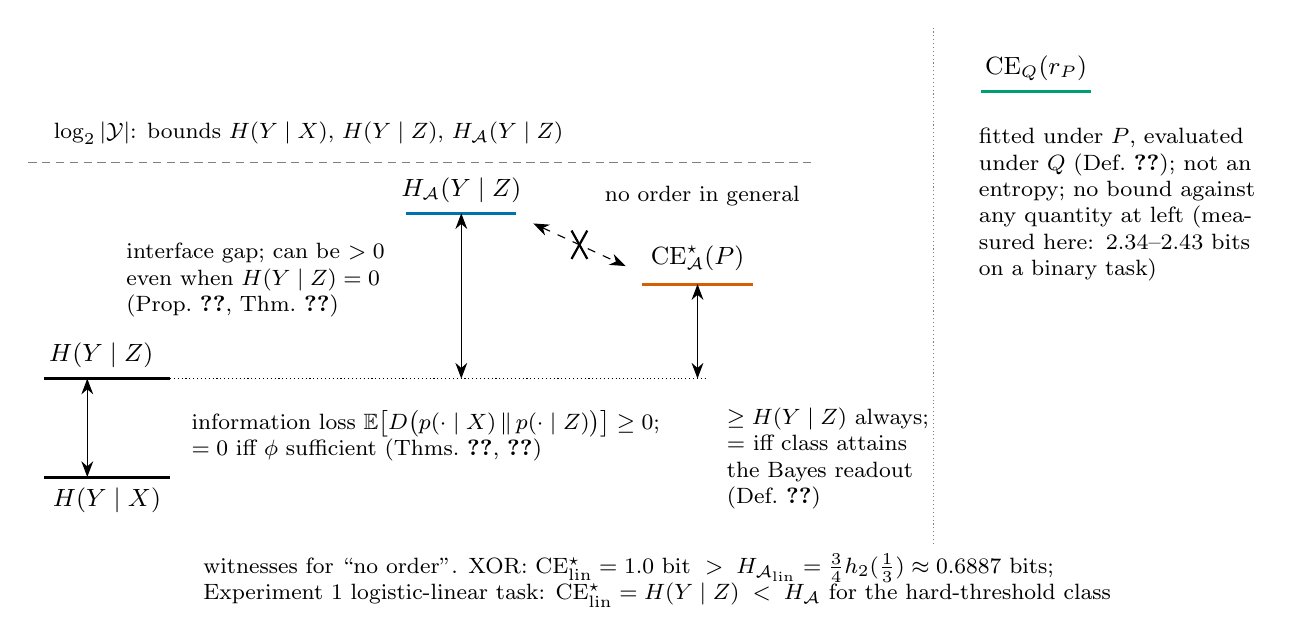
\begin{tikzpicture}[
  >={Stealth[length=2mm]},
  level/.style={line width=1.1pt},
  gaparrow/.style={<->},
  lab/.style={font=\small},
  note/.style={font=\footnotesize, align=left}
]
% ---- entropy-bound line ----
\draw[densely dashed, gray] (-0.2,4.30) -- (9.8,4.30);
\node[note, anchor=south west] at (0,4.40)
  {$\log_2|\cY|$: bounds $H(Y \mid X)$, $H(Y \mid Z)$,
   $H_{\cA}(Y \mid Z)$};
% ---- left block: the two entropies ----
\draw[level] (0,0.30) -- (1.6,0.30)
  node[midway, below, lab] {$H(Y \mid X)$};
\draw[level] (0,1.55) -- (1.6,1.55)
  node[at start, above right, lab, xshift=-2pt] {$H(Y \mid Z)$};
\draw[densely dotted, thin] (1.6,1.55) -- (8.4,1.55);
\draw[gaparrow] (0.55,0.30) -- (0.55,1.55);
\node[note, anchor=west] at (1.75,0.82)
  {information loss
   $\E\big[D\big(p(\cdot \mid X)\,\|\,p(\cdot \mid Z)\big)\big] \ge 0$;\\
   $= 0$ iff $\phi$ sufficient
   (Thms.~\ref{thm:lawful-preserve}, \ref{thm:unlawful-cost})};
% ---- hard readout-constrained quantity ----
\draw[level, okblue] (4.6,3.65) -- (6.0,3.65)
  node[midway, above, lab, black] {$H_{\cA}(Y \mid Z)$};
\draw[gaparrow] (5.3,1.55) -- (5.3,3.65);
\node[note, anchor=east] at (4.45,2.80)
  {interface gap; can be $> 0$\\
   even when $H(Y \mid Z) = 0$\\
   (Prop.~\ref{prop:xor-floor},
    Thm.~\ref{thm:superposition})};
% ---- soft population optimum ----
\draw[level, okverm] (7.6,2.75) -- (9.0,2.75)
  node[midway, above, lab, black, yshift=1pt] {$\CE^{\star}_{\cA}(P)$};
\draw[gaparrow] (8.3,1.55) -- (8.3,2.75);
\node[note, anchor=north west] at (8.55,1.30)
  {$\ge H(Y \mid Z)$ always;\\
   $=$ iff class attains\\
   the Bayes readout\\
   (Def.~\ref{def:cestar})};
% ---- the struck non-relation ----
\draw[dashed, <->, shorten <=2pt, shorten >=2pt]
  (6.15,3.55) -- (7.45,2.95) coordinate[midway] (mid);
\draw[thick] ($(mid)+(-0.10,-0.18)$) -- ($(mid)+(0.10,0.18)$);
\draw[thick] ($(mid)+(0.10,-0.18)$) -- ($(mid)+(-0.10,0.18)$);
\node[note, anchor=south west] at (7.0,3.62)
  {no order in general};
\node[note, anchor=north west] at (1.9,-0.55)
  {witnesses for ``no order''. XOR:
    $\CE^{\star}_{\mathrm{lin}} = 1.0$ bit $\;>\;
    H_{\Alin} = \tfrac34 h_2(\tfrac13) \approx 0.6887$ bits;\\
   Experiment 1 logistic-linear task:
    $\CE^{\star}_{\mathrm{lin}} = H(Y \mid Z) \;<\;
     H_{\cA}$ for the hard-threshold class};
% ---- the off-scale transfer quantity ----
\draw[densely dotted, gray] (11.3,-0.55) -- (11.3,6.0);
\draw[level, okgreen] (11.9,5.20) -- (13.3,5.20)
  node[midway, above, lab, black] {$\CEQ{\rP}$};
\node[note, anchor=north west, text width=3.5cm] at (11.75,4.85)
  {fitted under $P$, evaluated under $Q$
   (Def.~\ref{def:ceq}); not an entropy;
   no bound against any quantity at left
   (measured here: $2.34$--$2.43$ bits
   on a binary task)};
\end{tikzpicture}
\caption{The four evaluation quantities of
Section~\ref{sec:three-quantities} and their exact relations (vertical
position = bits, schematic, not to scale). Double-headed vertical arrows
are the two proved gaps and the soft-optimum excess; the struck dashed
arrow records that $H_{\cA}(Y \mid Z)$ and $\CE^{\star}_{\cA}(P)$ admit
\emph{no} order in general, with both witnesses shown ($1.0$ vs.\
$0.6887$ bits for XOR, and the reverse strict order on the Experiment~1
logistic-linear construction). $\CEQ{\rP}$, right of the dotted
separator, is the only quantity evaluated under a shifted distribution
$Q$; it obeys no entropy bound and in Section~\ref{sec:exp1} exceeds
the $1$-bit binary bound by construction-predicted amounts.}
\label{fig:quantities}
\end{figure*}


\paragraph{Roadmap.} Section~\ref{sec:setup} fixes definitions,
Sections~\ref{sec:lawful} and \ref{sec:readout} carry the theory
(steps 3 and 4), Section~\ref{sec:experiments} the pre-registered
measurements (step 5; the measurement discipline is stated there
once, in full), and Section~\ref{sec:discussion} the reporting
recommendation (step 6).

\section{Setup and Definitions}
\label{sec:setup}

\subsection{Spaces, random variables, and standing assumptions}

Let $(\Omega, \mathcal F, P)$ be a probability space carrying an input $X$
with values in a standard Borel space $(\cX, \mathcal B_{\cX})$, a task
target $Y$ with values in a finite alphabet $\cY$, and a measurable map
$\phi : \cX \to \cZ$ into a standard Borel space, with
$Z = \phi(X)$. Standing assumptions:

\begin{itemize}
\item[\textbf{(A1)}] $|\cY| < \infty$, so $H(Y) \le \log_2 |\cY| < \infty$
and all conditional entropies below are finite. (Everything extends
verbatim to countable $\cY$ with $H(Y) < \infty$; for general alphabets the
mutual-information statements survive with the general definition of $I$
\cite{polyanskiywu}, while the conditional-entropy phrasing requires
differential-entropy caveats and is not asserted.)
\item[\textbf{(A2)}] No side channel: $Z$ is produced from $X$ alone. For
deterministic $\phi$ this is automatic; for a stochastic representation
(a Markov kernel from $\cX$ to $\cZ$) it is the structural requirement that
$Y \to X \to Z$ is a Markov chain. Without (A2) the results are false and
uninteresting ($Z = Y$ is not a representation of $X$).
\end{itemize}

Since $\cX$ and $\cZ$ are standard Borel, regular conditional distributions
exist \cite{kallenberg}; fix versions $p(y \mid x) = P(Y = y \mid X = x)$
and $p(y \mid z) = P(Y = y \mid Z = z)$, defined $P_X$- and $P_Z$-almost
everywhere. Logarithms are base 2 (bits), $0 \log 0 = 0$, and
$\hb(p) = -p \log_2 p - (1-p)\log_2(1-p)$ is binary entropy.

\subsection{Four evaluation quantities}
\label{sec:three-quantities}

The four quantities of the introduction, now precisely. The first two
are distribution-level entropies; the third is a property of a
\emph{fitted} interface and is not an entropy at all; the fourth is a
population optimum over a soft readout class, the object the
in-distribution experiments estimate. Conflating any two of them
produces wrong conclusions: Section~\ref{sec:exp1} measures three of
the four (all but a hard-class $H_{\cA}$), and
Remark~\ref{rem:sufficient-hurts} separates the first two by theorem.

\paragraph{(1) Task-conditional entropy.} Task-relevant uncertainty after
representation is Shannon conditional entropy for the task's own target:
\begin{gather*}
H(Y \mid Z) = \E\big[\cH(p(\cdot \mid Z))\big],
\\
\cH(\mu) = -\textstyle\sum_{y \in \cY} \mu(y)\log \mu(y).
\end{gather*}
This quantity is a property of the pair $(Y, Z)$ alone: no interface, no
training. It satisfies $H(Y \mid Z) \le \log_2 |\cY|$ and is governed by
the sufficiency dichotomy of Section~\ref{sec:lawful}.

\paragraph{(2) Readout-constrained task uncertainty.}

\begin{definition}[readout-constrained task uncertainty]
\label{def:ha}
For a representation $Z$ and a class $\cA$ of measurable maps on $\cZ$,
\[
H_{\cA}(Y \mid Z) := \inf_{r \in \cA} H\big(Y \mid r(Z)\big).
\]
\end{definition}

Since each $r(Z)$ is a function of $Z$, the data-processing inequality gives
$H_{\cA}(Y \mid Z) \ge H(Y \mid Z)$ always, with equality whenever $\cA$
contains a readout sufficient for $Y$ given $Z$ (e.g.\ the identity).
Conditioning is on the $\sigma$-algebra $\sigma(r(Z))$; in particular a
binary readout and its complement induce the same partition, so
$H(Y \mid r(Z)) = H(Y \mid 1 - r(Z))$. The output cardinality of the class
is part of its declaration; the parametric classes in this paper have binary
outputs. $H_{\cA}$ is still a population infimum (the best the class can
do, not what any particular training run finds) and still satisfies
$H_{\cA}(Y \mid Z) \le \log_2 |\cY|$ (the constant readout is available in
every class considered here). It is
governed by the interface-floor results of Section~\ref{sec:readout}.

\paragraph{(3) Frozen-readout transfer cross-entropy.}

\begin{definition}[frozen-readout transfer cross-entropy]
\label{def:ceq}
Let $\rP$ be a probabilistic readout (a measurable map $z \mapsto
q_{\rP}(\cdot \mid z)$, a distribution over $\cY$) selected (trained,
calibrated, or population-optimized) using the distribution $P$, and let
$Q$ be an evaluation distribution for $(Z, Y)$. The \emph{transfer
cross-entropy} of the frozen readout is
\[
\CEQ{\rP} := \E_{Q}\big[-\log q_{\rP}(Y \mid Z)\big].
\]
\end{definition}

Three properties make this a different object from (1) and (2).
First, it depends on the fitted interface $\rP$, hence on the fitting
distribution $P$, not only on the pair $(Y, Z)$ under $Q$. Second, it obeys
no entropy bound: $\CEQ{\rP}$ can exceed $\log_2 |\cY|$ arbitrarily (and in
Section~\ref{sec:exp1} it does: post-shift values of $2.34$--$2.43$
bits for a binary task; in Section~\ref{sec:exp3}, $4.77$ bits against
the $\log_2 10 \approx 3.32$-bit ten-class bound). Third, it does not lower-bound or upper-bound
$H_{\cA}(Y \mid Z)$ under $Q$ in general: a readout refit under $Q$
(its population optimum is $\CE^{\star}_{\cA, Q}$,
Definition~\ref{def:cestar} applied under $Q$) can sit far below
$\CEQ{\rP}$. The gap $\CEQ{\rP} - \CE^{\star}_{\cA, Q}$ is \emph{transfer
risk} of the frozen interface, a deployment property, not an information
property.

\paragraph{(4) Population soft-readout optimum.}

\begin{definition}[population soft-readout cross-entropy optimum]
\label{def:cestar}
For a class $\cA_{\mathrm{soft}}$ of probabilistic readouts
$q : z \mapsto q(\cdot \mid z)$ (each a distribution over $\cY$; the
cross-entropy is extended-real, taking the value $+\infty$ when $q$
assigns zero mass to a realized label), the
\emph{population soft-readout optimum} under $P$ is
\[
\CE^{\star}_{\cA}(P) := \inf_{q \in \cA_{\mathrm{soft}}}
\E_P\big[-\log q(Y \mid Z)\big].
\]
\end{definition}

$\CE^{\star}_{\cA}$ is, up to notation and convention, the conditional
$\mathcal{V}$-entropy of Xu et al.~\cite{xuvinfo} for
$\mathcal{V} = \cA_{\mathrm{soft}}$; see
Section~\ref{sec:related}.

The relations to the first two quantities are exact and asymmetric. For
every probabilistic readout $q$,
\begin{multline*}
\E_P\big[-\log q(Y \mid Z)\big]
= H(Y \mid Z) \\
+ \E_P\big[D\big(p(\cdot \mid Z) \,\big\|\,
q(\cdot \mid Z)\big)\big] \;\ge\; H(Y \mid Z),
\end{multline*}
so $\CE^{\star}_{\cA} \ge H(Y \mid Z)$ always, with equality when the
class contains (or approaches) the Bayes readout $p(\cdot \mid z)$. But
$\CE^{\star}_{\cA}$ does \emph{not} in general bound
$H_{\cA'}(Y \mid Z)$ for a hard deterministic class $\cA'$, in either
direction: a soft score is not a hard partition plus per-cell
calibration. Both witnesses are recorded in
Figure~\ref{fig:quantities}: for the XOR task of
Proposition~\ref{prop:xor-floor}, $\CE^{\star}_{\mathrm{lin}} = 1$ bit
exactly (the objective is convex and stationary at $w = 0$, $b = 0$),
strictly \emph{above} the hard floor
$\tfrac34 \hb(\tfrac13) \approx 0.6887$ bits; when $Y \mid Z$ is
logistic-linear (the Experiment~1 construction),
$\CE^{\star}_{\mathrm{lin}} = H(Y \mid Z)$, strictly \emph{below} the
hard-threshold class's $H_{\cA}$. The experiments never assume the
two objects coincide.

\paragraph{Measured quantities, and the bridge.} The experiments of
Section~\ref{sec:experiments} measure held-out cross-entropies of
trained soft readouts, written with the symbol $\CE$ throughout:
$\CEhat_{\mathrm{ID}}$ for the in-distribution held-out cross-entropy
of a readout trained and evaluated under $P$, and $\CEhat_{Q}(\rP)$
for the measured transfer cross-entropy under shift. The symbols $H$
and $H_{\cA}$ are reserved for the theorem-side quantities;
$\CE^{\star}_{\cA}$ (Definition~\ref{def:cestar}) is what the
in-distribution measurements estimate. The bridge is the identity
displayed above: the \emph{population} cross-entropy risk of a
probabilistic readout
upper-bounds $H(Y \mid Z)$, but never, in general, a hard-class
$H_{\cA}$; the measured held-out $\CEhat$ is a finite-sample estimate
of that risk and may fluctuate below it. We treat $\CEhat$ as an
estimate of its declared target $\CE^{\star}_{\cA}$ (and, where the
soft class provably contains the Bayes readout, of $H(Y \mid Z)$
itself) only where the estimator has been validated against analytic
ground truth, which the in-distribution validation steps of
Section~\ref{sec:experiments} establish, to within the predicted
maximum-likelihood estimation bias. No such validation is possible
post-shift, which is why post-shift numbers are reported as
$\CEQ{\rP}$ and never as entropies. Figure~\ref{fig:quantities} draws
the four quantities with exactly these relations.


\subsection{Lawfulness as sufficiency}

\begin{definition}[lawful compression]
\label{def:lawful}
$\phi$ is \emph{lawful} (sufficient) for $Y$ if
$p(y \mid x) = p(y \mid \phi(x))$ for $P_X$-a.e.\ $x$ and every
$y \in \cY$. Writing
$A := \{x \in \cX : p(\cdot \mid x) \neq p(\cdot \mid \phi(x))\}$,
$\phi$ is \emph{non-sufficient} iff $P_X(A) > 0$.
\end{definition}

A discrepancy confined to a $P_X$-null set is invisible to every quantity in
this paper and counts as sufficiency; this null-set convention is exactly
what makes Theorems~\ref{thm:lawful-preserve} and \ref{thm:unlawful-cost} an
exhaustive dichotomy.

\subsection{Accounting conventions for \texorpdfstring{$K$}{K} and \texorpdfstring{$E$}{E}}
\label{sec:ke-conventions}

Throughout, $K$ denotes counted stored structure (parameter counts,
codebook entries) and $E$ counted operations (FLOPs per evaluation or per
training run), each under a convention stated before use and, in the
experiments, committed before any run. These are declared bookkeeping, not
mathematics: different conventions give different constants, and we will be
explicit about which statements are convention-robust and which are not.

\paragraph{Two stored-parameter conventions.} For the circuit families
of Section~\ref{sec:readout}, two stored-parameter counts arise and
must not be conflated. The \emph{unshared count} $\Kunsh$ counts every
gate coefficient and bias separately, whether or not stored values
coincide numerically; the \emph{distinct-value count} $\Kval$ counts
distinct stored values once, however often a value is reused. Where a
claim depends on the convention we write $\Kunsh$ or $\Kval$
explicitly; a bare $K$ appears only where the convention in force has
just been declared (as in each experiment's committed accounting) or
where the two counts coincide.

\paragraph{Scope.} The composite objective $\cR = K + H_\cT + \lambda E$
appears only in Corollary~\ref{cor:accounting}, where $\lambda$ enters as a
declared conversion rate between accounting units, quantified over and never
assigned a value.

\section{Lawful Compression: the Exact Dichotomy}
\label{sec:lawful}

Nothing in this section is new mathematics, and the paper does not
rest on it for novelty: it is a clean restatement of the standard
sufficiency/DPI equality conditions
\cite{coverthomas,kullback,polyanskiywu}, organized (null-set
discipline, explicit divergence form of the gap, and the accounting
corollary) for the cost-accounting question the rest of the paper
asks. The exact statements matter because the experiments of
Section~\ref{sec:experiments} are checked against them and the
precision (a.s.\ conventions, which quantity is governed by which
theorem) is load-bearing there; the proofs, which are classical, are
relocated to Appendix~\ref{app:proofs-s3}.

\begin{lemma}[sufficiency $\Leftrightarrow$ conditional independence]
\label{lem:ci}
$\phi$ is sufficient for $Y$ (Definition~\ref{def:lawful}) if and only if
$Y \perp X \mid Z$, i.e.\ $P(Y = y \mid X, Z) = P(Y = y \mid Z)$ a.s.\ for
every $y$.
\end{lemma}

\begin{lemma}[divergence identity]
\label{lem:divergence}
Under (A1)--(A2), with $Z = \phi(X)$,
\begin{multline}
\label{eq:divergence}
H(Y \mid Z) - H(Y \mid X) \\
= \E\Big[D\big(p(\cdot \mid X) \,\big\|\, p(\cdot \mid Z)\big)\Big]
\;\in\; [0, \log_2 |\cY|],
\end{multline}
where $D(\mu \| \nu) = \sum_y \mu(y) \log \frac{\mu(y)}{\nu(y)}$ is relative
entropy.
\end{lemma}

Identity \eqref{eq:divergence} is the equality-condition form of the
data-processing inequality specialized to this setup: the right side equals
$I(Y; X \mid Z)$, and the chain rule
$I(Y; X) = I(Y; Z) + I(Y; X \mid Z)$ together with $I(Y; Z \mid X) = 0$
(which is (A2)) recovers the DPI $I(Y; Z) \le I(Y; X)$
\cite[Thm.~2.8.1]{coverthomas}. Both theorems below fall out of
\eqref{eq:divergence} with no further work.

\begin{theorem}[sufficient compression is free]
\label{thm:lawful-preserve}
Assume (A1)--(A2) and let $Z = \phi(X)$. The data-processing inequality
always gives $H(Y \mid Z) \ge H(Y \mid X)$ and $I(Y; Z) \le I(Y; X)$. If
$\phi$ is sufficient for $Y$, both hold with equality:
\[
H(Y \mid Z) = H(Y \mid X), \qquad I(Y; Z) = I(Y; X).
\]
\end{theorem}

\begin{theorem}[insufficient compression strictly costs]
\label{thm:unlawful-cost}
Assume (A1)--(A2) and let $Z = \phi(X)$. If $\phi$ is not sufficient for
$Y$, that is, $P_X(A) > 0$ for
$A = \{x : p(\cdot \mid x) \neq p(\cdot \mid \phi(x))\}$, then
\[
H(Y \mid Z) > H(Y \mid X), \qquad I(Y; Z) < I(Y; X).
\]
\end{theorem}

\begin{remark}[null-set precision and exhaustiveness]
The dichotomy is exhaustive and exclusive because of the a.s.\ convention in
Definition~\ref{def:lawful}: discrepancy on a $P_X$-null set means
sufficiency holds with a modified version and
Theorem~\ref{thm:lawful-preserve} applies; discrepancy on a
positive-probability set means Theorem~\ref{thm:unlawful-cost} applies.
There is no intermediate case, and combining the two with
Lemma~\ref{lem:ci} gives the standard DPI equality condition:
$H(Y \mid Z) = H(Y \mid X)$ iff $Y \perp X \mid Z$.
\end{remark}

Both theorems extend verbatim to stochastic representation maps
(Markov kernels), with sufficiency generalized to $Y \perp X \mid Z$
(Remark~\ref{rem:stochastic}, Appendix~\ref{app:proofs-s3}).

\subsection{Sufficiency does not imply achievability: the XOR floor}
\label{sec:xor-floor}

Sufficiency says nothing about what a restricted readout class can extract.
The following proposition makes that gap exact, with the classical XOR
example \cite{minskypapert} pushed through to the entropy floor; the
proof (a finite enumeration, tabulated in Appendix~\ref{app:enum-xor})
is in Appendix~\ref{app:proofs-s3}.

\begin{proposition}[XOR floor under linear-threshold readouts]
\label{prop:xor-floor}
Let $X = (X_1, X_2)$ be uniform on $\{0,1\}^2$, $Y = X_1 \oplus X_2$, and
$Z = X$ (the identity, trivially sufficient, so $H(Y \mid Z) = 0$). Let
\[
\Alin
= \big\{z \mapsto \mathbf 1\{w_1 z_1 + w_2 z_2 \ge \theta\}
  \;:\; w \in \R^2,\ \theta \in \R\big\}.
\]
Then
\begin{multline*}
H_{\Alin}(Y \mid Z)
= \tfrac34\, \hb\!\big(\tfrac13\big)
= \tfrac34 \log_2 3 - \tfrac12 \\
\approx 0.6887 \text{ bits}
\;>\; 0 = H(Y \mid Z),
\end{multline*}
and in error-probability terms: Bayes error from $Z$ is $0$, while the best
error achievable through any $\Alin$-readout is $1/4$.
\end{proposition}

\begin{remark}[sufficient compression can strictly degrade the interface]
\label{rem:sufficient-hurts}
Theorem~\ref{thm:lawful-preserve} does \emph{not} survive the substitution
$H \mapsto H_{\cA}$. Let $X' = (X_1, X_2, X_1 \oplus X_2)$ with
$(X_1, X_2)$ uniform on $\{0,1\}^2$, $Y = X_1 \oplus X_2$, and
$\phi(X') = (X_1, X_2)$ (drop the redundant third coordinate). $\phi$ is
sufficient (the third coordinate is a function of the first two, so
$p(y \mid X') = p(y \mid \phi(X'))$ pointwise), yet with $\Alin$ the
class of linear-threshold readouts on the available coordinates,
\begin{gather*}
H_{\Alin}(Y \mid X') = 0,
\\
H_{\Alin}(Y \mid \phi(X')) = \tfrac34 \hb(\tfrac13) > 0,
\end{gather*}
the first by reading the third coordinate ($w = (0,0,1)$,
$\theta = \tfrac12$), the second by Proposition~\ref{prop:xor-floor}. Lawful compression preserved
$H(Y \mid \cdot)$ exactly while strictly degrading what the restricted
interface can extract. Lawfulness in the sense of
Definition~\ref{def:lawful} is a statement about information, not about
interface-accessible information; the two coincide only when $\cA$ is rich
enough (e.g.\ contains the Bayes readout for both representations). This
distinction is a design requirement for measurement: an experiment must
declare what its cross-entropy proxy targets: $H(Y \mid Z)$, a
hard-class $H_{\cA}(Y \mid Z)$, or a soft-class optimum
$\CE^{\star}_{\cA}$ (Definition~\ref{def:cestar}). The three
are governed by different statements.
All three experiments in Section~\ref{sec:experiments} declare it
(their declared target is $\CE^{\star}_{\cA}$ for the stated soft
class; in Experiment~3 only \emph{differences} of $\CE^{\star}$ are
validated, Section~\ref{sec:exp3}).
\end{remark}

\subsection{Accounting consequence}

\begin{corollary}[$K$ and $E$ may drop freely under sufficiency]
\label{cor:accounting}
Let $M_X$ and $M_Z$ be representational processes operating on $X$ and on
$Z = \phi(X)$, with declared costs $(K(M_X), E(M_X))$ and
$(K(M_Z), E(M_Z))$, and let the task term be $H_\cT = H(Y \mid \cdot)$. If
$\phi$ is sufficient for $Y$, then the objective
$\cR = K + H_\cT + \lamvar E$ changes by
\[
\Delta\cR = \Delta K + \underbrace{\Delta H_\cT}_{=\,0
\ (\text{Thm.~\ref{thm:lawful-preserve}})} + \lamvar\, \Delta E,
\]
so any strict reduction in $K$ and/or $E$ (the other not increasing)
strictly reduces $\cR$ \emph{for every} $\lamvar \ge 0$, at exactly zero
task-relevant-uncertainty cost. Conversely, if $\phi$ is non-sufficient,
every such substitution pays $\Delta H_\cT > 0$
(Theorem~\ref{thm:unlawful-cost}), and whether $\cR$ decreases becomes a
quantitative trade-off rather than a free move.
\end{corollary}

This is bookkeeping given the theorems (it contains no new mathematics),
but it is the exact form in which the experiments of
Section~\ref{sec:experiments} check lawful-compression claims, and the
``for every $\lamvar \ge 0$'' quantifier is what allows the check to avoid
assigning $\lamvar$ any value.

\section{Readout Geometry: Exact Interface Floors and the Price of Beating Them}
\label{sec:readout}

This section carries the paper's theorem-side content. Here $Z$ is
fixed and the readout class varies. The first statement is trivial and
is labeled as such; the content is the exact strict gaps, the payment
analysis within the hidden-layer threshold ladder, the two
counterexamples that refute the universal forms of the accounting
claim (Section~\ref{sec:accounting}), and the payment frontier, closed
exactly for the superposition family (Section~\ref{sec:narrowed}).

\begin{proposition}[monotonicity under class inclusion]
\label{prop:monotone}
If $\cA_1 \subseteq \cA_2$, then
$H_{\cA_2}(Y \mid Z) \le H_{\cA_1}(Y \mid Z)$.
\end{proposition}

\begin{proof}
The infimum over a superset of a set of reals is no larger.
\end{proof}

The inequality can hold with equality under \emph{strict} inclusion
(Theorem~\ref{thm:superposition}(iii) proves an instance), so ``larger
readout classes need not help'' is itself theorem-backed.

\subsection{Declared parametric classes and their accounting}
\label{sec:classes}

The payment analysis needs declared, countable $K$ (stored parameters) and
$E$ (inference FLOPs per evaluation) per class. These are stated
conventions: a length-$d$ dot product costs $2d - 1$ FLOPs, subtracting a
threshold costs $1$, a comparison costs $1$. Every $K$ value in this
section and in the ladder declarations below is an \emph{unshared}
count, $K = \Kunsh$ in the Section~\ref{sec:ke-conventions} notation;
where value sharing changes a claim we mark the shared count $\Kval$
explicitly.

% Two-column layout: the class/definition/cost table re-set with one
% class per block (definition row, then K/E row); content identical.
\begin{center}
\small
\begin{tabular}{@{}l@{}}
\toprule
$\Alin(d)$: \quad $z \mapsto \mathbf 1\{w \cdot z \ge \theta\}$ \\
\hspace*{1.2em}$K = d + 1$, \quad $E = 2d + 1$ \\
\addlinespace
$\Athr{m}(d)$: \quad
$z \mapsto \mathbf 1\{\sum_{i=1}^m v_i\, g_i(z) + c \ge 0\}$ \\
\hspace*{1.2em}$K = m(d{+}1) + (m{+}1)$, \quad
$E = m(2d{+}1) + (2m{+}1)$ \\
\bottomrule
\end{tabular}
\end{center}

\noindent
where each hidden unit is itself a linear threshold,
$g_i(z) = \mathbf 1\{w_i \cdot z \ge \theta_i\}$. We call the family
$\{\Athr{m}(d)\}_m$ the \emph{hidden-layer threshold ladder}: the
output unit reads the hidden units \emph{only}: no unit reads a raw
coordinate of $z$ alongside hidden-unit outputs. This is the family for
which the payment floors of Proposition~\ref{prop:payment} are proved;
it must not be confused with the strictly more permissive
\emph{affine-threshold compositions} $\cA_{\mathrm{comp}}(d)$ of
Definition~\ref{def:acomp}, whose gates may read raw coordinates and
earlier gates together.

$\Alin(d) \subseteq \Athr{1}(d) \subseteq \Athr{2}(d) \subseteq \cdots$: a
linear threshold is realized with one hidden unit, and a zero-weight hidden
unit embeds $\Athr{m}$ into $\Athr{m+1}$; constants are in $\Alin$
($w = 0$). Instance values used below: $\Alin(1)$: $K = 2$, $E = 3$;
$\Athr{2}(1)$: $K = 7$, $E = 11$; $\Athr{3}(1)$: $K = 10$, $E = 16$;
$\Alin(2)$: $K = 3$, $E = 5$; $\Athr{2}(2)$: $K = 9$, $E = 15$.

\begin{definition}[declared readout ladder]
\label{def:ladder}
A \emph{declared readout ladder} is a finite chain
$\cA_1 \subseteq \cdots \subseteq \cA_L$ of readout classes together with
declared accounting values $K_1 < \cdots < K_L$ and $E_1 < \cdots < E_L$
under a stated convention, strictly increasing along the chain \emph{by
construction}.
\end{definition}

The strict monotonicity of $K$ and $E$ along a ladder is part of the
declaration, not a derived fact; the definition exists so that
Section~\ref{sec:accounting} can state exactly what is and is not claimed.

\subsection{Family 1: XOR, and the gap closed at width 2}

\begin{lemma}[single-hidden-unit collapse]
\label{lem:collapse}
For every $(Y, Z)$ and every $d$:
$H_{\Athr{1}(d)}(Y \mid Z) = H_{\Alin(d)}(Y \mid Z)$.
\end{lemma}

\begin{proof}
Let $r \in \Athr{1}(d)$, $r(z) = \mathbf 1\{v_1 g_1(z) + c \ge 0\}$ with
$g_1 \in \Alin(d)$. As $g_1(z) \in \{0, 1\}$, $r$ is a constant, $g_1$, or
$1 - g_1$. Constants give $H(Y \mid r(Z)) = H(Y)$, achievable in $\Alin$;
$g_1 \in \Alin$; and $1 - g_1$ induces the same partition as $g_1$. So the
infima over the two classes run over the same set of values.
\end{proof}

\begin{theorem}[XOR gap, exact]
\label{thm:xor-gap}
Let $X = (X_1, X_2)$ uniform on $\{0,1\}^2$, $Y = X_1 \oplus X_2$,
$Z = X$, as in Proposition~\ref{prop:xor-floor}. Take
$\cA_1 = \Alin(2)$, $\cA_2 = \Athr{2}(2)$ (strict inclusion). Then
\begin{gather*}
H_{\cA_1}(Y \mid Z) = \tfrac34 \hb\big(\tfrac13\big) \approx 0.6887
\text{ bits},
\\
H_{\cA_2}(Y \mid Z) = 0,
\end{gather*}
so the gap is exactly $\tfrac34 \hb(\tfrac13)$ bits, attained.
\end{theorem}

\begin{proof}
The first equality is Proposition~\ref{prop:xor-floor}. For the second, the
two-hidden-unit threshold network with
$g_1 = \mathbf 1\{z_1 + z_2 \ge 1\}$, $g_2 = \mathbf 1\{z_1 + z_2 \ge 2\}$,
output $\mathbf 1\{g_1 - g_2 - 1 \ge 0\}$, computes XOR exactly on
$\{0,1\}^2$: $(0,0) \mapsto (0,0) \mapsto 0$;
$(0,1), (1,0) \mapsto (1,0) \mapsto 1$; $(1,1) \mapsto (1,1) \mapsto 0$.
Hence $H(Y \mid r(Z)) = 0$ for this $r \in \cA_2$, and
$H_{\cA_2}(Y \mid Z) \ge H(Y \mid Z) = 0$ gives equality.
\end{proof}

Figure~\ref{fig:xor-geometry} shows both halves of the XOR story:
panel (a) the $3$-vs-$1$ split behind the $\tfrac34 h_2(\tfrac13)$
floor, with the diagonal pair unreachable by any line; panel (b) the
quadratic decoder of Proposition~\ref{prop:quadratic}
(Section~\ref{sec:disproofs}), which folds the plane about the
diagonal and separates XOR with one threshold.

\begin{figure}[t]
\centering
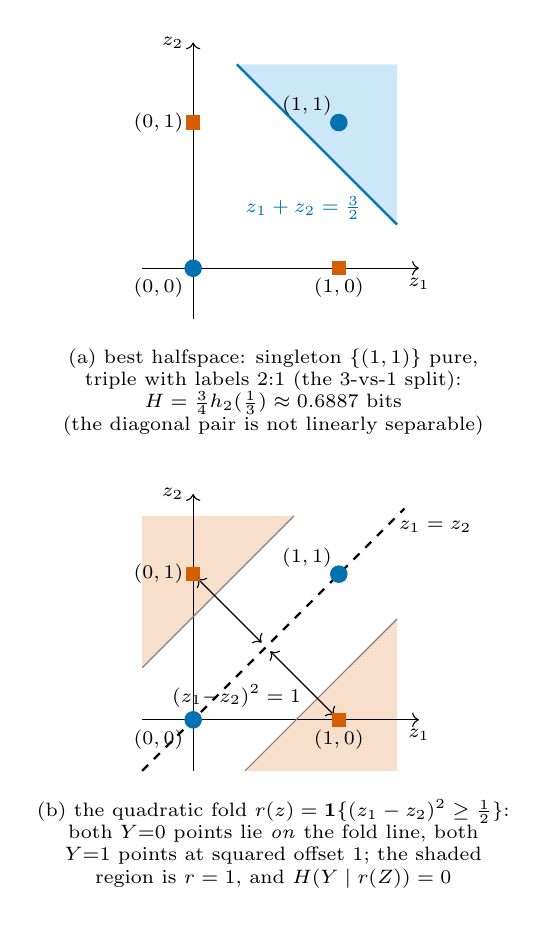
\begin{tikzpicture}[scale=1.85,
  y0/.style={circle, draw=okblue, fill=okblue, inner sep=2.1pt},
  y1/.style={rectangle, draw=okverm, fill=okverm, inner sep=2.4pt},
  ptlab/.style={font=\scriptsize},
  note/.style={font=\scriptsize, align=center}]
% ---------------- panel (a): best halfspace ----------------
\begin{scope}
\fill[oksky!30] (0.30,1.40) -- (1.40,0.30) -- (1.40,1.40) -- cycle;
\draw[->] (-0.35,0) -- (1.55,0) node[below, ptlab] {$z_1$};
\draw[->] (0,-0.35) -- (0,1.55) node[left, ptlab] {$z_2$};
\draw[okblue, thick] (0.30,1.40) -- (1.40,0.30)
  node[pos=0.80, anchor=north east, ptlab, inner sep=1pt]
  {$z_1 + z_2 = \tfrac32$};
\node[y0] at (0,0) {}; \node[ptlab, below left] at (0,0) {$(0,0)$};
\node[y1] at (0,1) {}; \node[ptlab, left] at (0,1) {$(0,1)$};
\node[y1] at (1,0) {}; \node[ptlab, below] at (1,0) {$(1,0)$};
\node[y0] at (1,1) {}; \node[ptlab, above left=-1pt] at (1,1) {$(1,1)$};
\node[note] at (0.55,-0.85)
  {(a) best halfspace: singleton $\{(1,1)\}$ pure,\\
   triple with labels $2{:}1$ (the $3$-vs-$1$ split):\\
   $H = \tfrac34 h_2(\tfrac13) \approx 0.6887$ bits\\
   (the diagonal pair is not linearly separable)};
\end{scope}
% ---------------- panel (b): quadratic fold ----------------
% (two-column layout: panels stacked vertically to fit one column)
\begin{scope}[yshift=-3.1cm]
% decision-1 corner regions: |z1 - z2| >= 1/sqrt2 (~0.7071)
\fill[okverm!20] (0.357,-0.35) -- (1.40,-0.35) -- (1.40,0.693) -- cycle;
\fill[okverm!20] (-0.35,0.357) -- (-0.35,1.40) -- (0.693,1.40) -- cycle;
\draw[->] (-0.35,0) -- (1.55,0) node[below, ptlab] {$z_1$};
\draw[->] (0,-0.35) -- (0,1.55) node[left, ptlab] {$z_2$};
\draw[dashed, thick] (-0.35,-0.35) -- (1.45,1.45)
  node[pos=0.93, right=1pt, ptlab] {$z_1 = z_2$};
\draw[gray, thin] (0.357,-0.35) -- (1.40,0.693);
\draw[gray, thin] (-0.35,0.357) -- (0.693,1.40);
\draw[<->, thin] (0.97,0.03) -- (0.53,0.47)
  node[midway, below left=-3pt, ptlab] {$(z_1{-}z_2)^2 = 1$};
\draw[<->, thin] (0.03,0.97) -- (0.47,0.53);
\node[y0] at (0,0) {}; \node[ptlab, below left] at (0,0) {$(0,0)$};
\node[y1] at (0,1) {}; \node[ptlab, left] at (0,1) {$(0,1)$};
\node[y1] at (1,0) {}; \node[ptlab, below] at (1,0) {$(1,0)$};
\node[y0] at (1,1) {}; \node[ptlab, above left=-1pt] at (1,1) {$(1,1)$};
\node[note] at (0.55,-0.85)
  {(b) the quadratic fold
   $r(z) = \mathbf 1\{(z_1 - z_2)^2 \ge \tfrac12\}$:\\
   both $Y{=}0$ points lie \emph{on} the fold line, both\\
   $Y{=}1$ points at squared offset $1$; the shaded\\
   region is $r = 1$, and $H(Y \mid r(Z)) = 0$};
\end{scope}
\end{tikzpicture}
\caption{The XOR geometry. Circles: $Y = 0$; squares: $Y = 1$; all four
points have mass $\tfrac14$. (a) The exact linear-threshold floor of
Proposition~\ref{prop:xor-floor}: the best achievable halfspace cell is a
pure singleton against a $2{:}1$ triple, giving
$\tfrac34 h_2(\tfrac13) \approx 0.6887$ bits, and the only partition that
would do better (diagonal pair vs.\ diagonal pair) is exactly the
non-achievable one. (b) The in-basis quadratic decoder of
Proposition~\ref{prop:quadratic}: $(z_1 - z_2)^2$ measures squared
offset from the diagonal $z_1 = z_2$, collapsing each diagonal class to
a single value ($0$ and $1$), so one threshold at $\tfrac12$ computes
XOR exactly.}
\label{fig:xor-geometry}
\end{figure}

\subsection{Family 2: sparse superposed features, with an equality rung}
\label{sec:superposition}

\paragraph{The family.} $\dfeat$ binary features with exactly $k$ active:
$F$ uniform on $\{f \in \{0,1\}^{\dfeat} : \sum_j f_j = k\}$. A fixed
projection $A \in \R^{\dz \times \dfeat}$ with $\dz < \dfeat$ superposes
them, $Z = AF$, and the task reads one designated feature, $Y = F_{j^*}$.
If $\operatorname{spark}(A) > 2k$ (every $2k$ columns linearly
independent), then $F \mapsto AF$ is injective on $k$-sparse vectors
\cite{donohoelad}, hence $H(F \mid Z) = 0$ and a fortiori
$H(Y \mid Z) = 0$: the representation is perfectly sufficient and all
readout-constrained uncertainty is interface-induced cross-talk. (Efficient
sparse recovery under incoherence is also classical \cite{tropp}, cited for
context on achievability cost, not used in any proof.)

\paragraph{The minimal computed instance.} $\dfeat = 4$, $k = 2$,
$\dz = 1$, $A = (1\;\,2\;\,4\;\,8)$, $Y = F_1$. The six equiprobable
feature patterns give six distinct sums (atoms):

\begin{center}
\footnotesize
\setlength{\tabcolsep}{3.4pt}
\begin{tabular}{lcccccc}
\toprule
$z$ & 3 & 5 & 6 & 9 & 10 & 12 \\
\midrule
active pair & $\{1,2\}$ & $\{1,3\}$ & $\{2,3\}$ & $\{1,4\}$ & $\{2,4\}$ & $\{3,4\}$ \\
$y = f_1$ & 1 & 1 & 0 & 1 & 0 & 0 \\
\bottomrule
\end{tabular}
\end{center}

All sums distinct $\Rightarrow$ $H(F \mid Z) = 0 \Rightarrow
H(Y \mid Z) = 0$ (injectivity verified directly for this instance). The
label pattern along the sorted atoms is $(1,1,0,1,0,0)$: the $Y{=}1$ fiber
is \emph{interleaved} with the $Y{=}0$ fiber on the line, the
one-dimensional analogue of the XOR diagonal, produced by superposition
cross-talk rather than by parity. Figure~\ref{fig:superposition-line}
draws the instance: the interleaving, the best single threshold cut (the
floor of part (ii) below), and the three cuts that decode exactly (part
(iv)).

\begin{figure*}[t]
\centering
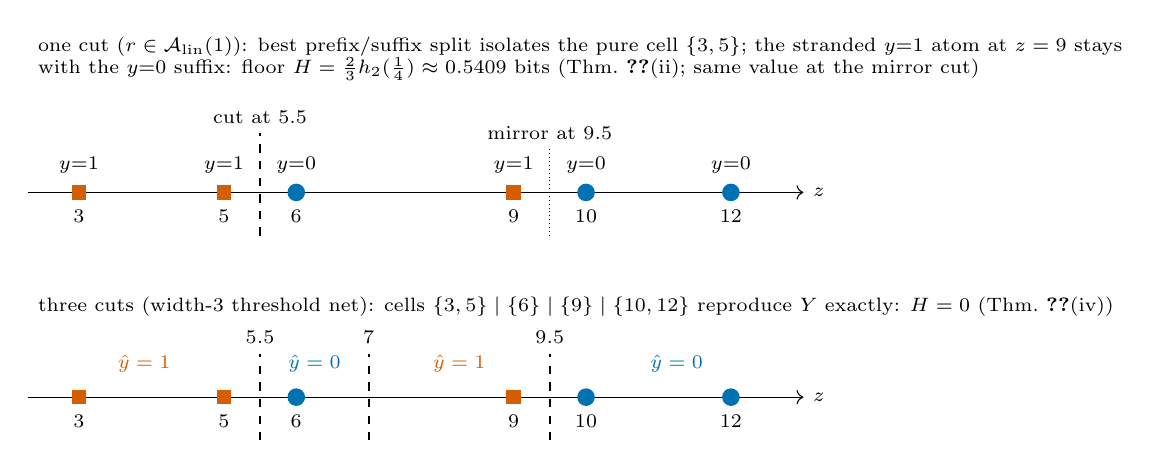
\begin{tikzpicture}[x=0.92cm, y=1cm,
  y0/.style={circle, draw=okblue, fill=okblue, inner sep=2.1pt},
  y1/.style={rectangle, draw=okverm, fill=okverm, inner sep=2.4pt},
  ptlab/.style={font=\scriptsize},
  note/.style={font=\scriptsize, align=left}]
% ----- top line: the linear floor (one cut) -----
\begin{scope}
\draw[->] (2.3,0) -- (13.0,0) node[right, ptlab] {$z$};
\foreach \z/\sty/\lbl in {3/y1/1, 5/y1/1, 6/y0/0, 9/y1/1, 10/y0/0, 12/y0/0}{
  \node[\sty] at (\z,0) {};
  \node[ptlab, below] at (\z,-0.10) {$\z$};
  \node[ptlab, above] at (\z,0.12) {$y{=}\lbl$};
}
\draw[dashed, thick] (5.5,-0.55) -- (5.5,0.75)
  node[above, ptlab] {cut at $5.5$};
\draw[densely dotted] (9.5,-0.55) -- (9.5,0.55)
  node[above, ptlab] {mirror at $9.5$};
\node[note, anchor=west] at (2.3,1.70)
  {one cut ($r \in \Alin(1)$): best prefix/suffix split isolates the pure
   cell $\{3,5\}$; the stranded $y{=}1$ atom at $z = 9$ stays\\
   with the $y{=}0$ suffix: floor
   $H = \tfrac23 h_2(\tfrac14) \approx 0.5409$ bits
   (Thm.~\ref{thm:superposition}(ii); same value at the mirror cut)};
\end{scope}
% ----- bottom line: width 3, exact decode -----
\begin{scope}[yshift=-2.6cm]
\draw[->] (2.3,0) -- (13.0,0) node[right, ptlab] {$z$};
\foreach \z/\sty in {3/y1, 5/y1, 6/y0, 9/y1, 10/y0, 12/y0}{
  \node[\sty] at (\z,0) {};
  \node[ptlab, below] at (\z,-0.10) {$\z$};
}
\foreach \c in {5.5, 7, 9.5}{
  \draw[dashed, thick] (\c,-0.55) -- (\c,0.55)
    node[above, ptlab] {$\c$};
}
\node[ptlab, okverm] at (3.9,0.42) {$\hat y = 1$};
\node[ptlab, okblue] at (6.25,0.42) {$\hat y = 0$};
\node[ptlab, okverm] at (8.25,0.42) {$\hat y = 1$};
\node[ptlab, okblue] at (11.25,0.42) {$\hat y = 0$};
\node[note, anchor=west] at (2.3,1.15)
  {three cuts (width-3 threshold net): cells $\{3,5\} \mid \{6\} \mid
   \{9\} \mid \{10,12\}$ reproduce $Y$ exactly: $H = 0$
   (Thm.~\ref{thm:superposition}(iv))};
\end{scope}
\end{tikzpicture}
\caption{The superposition line instance: six equiprobable atoms
$z \in \{3, 5, 6, 9, 10, 12\}$ (sums of the active column pairs of
$A = (1\;2\;4\;8)$) with labels $(1,1,0,1,0,0)$ in sorted order:
squares $y = 1$, circles $y = 0$. Top: any single linear threshold
realizes only prefix/suffix splits; the best one pays
$\tfrac23 h_2(\tfrac14) \approx 0.5409$ bits because the $y{=}1$ fiber
is interleaved. Two cuts provably do no better
(Thm.~\ref{thm:superposition}(iii)). Bottom: three cuts (the width-3
network of Thm.~\ref{thm:superposition}(iv)) isolate the stranded atom
at $z = 9$ and decode exactly.}
\label{fig:superposition-line}
\end{figure*}

\begin{theorem}[superposition gap, exact, with an equality rung]
\label{thm:superposition}
For the instance above:
\begin{enumerate}
\item[(i)] $H(Y \mid Z) = 0$.
\item[(ii)] $H_{\Alin(1)}(Y \mid Z) = \tfrac23 \hb(\tfrac14)
= \tfrac43 - \tfrac12 \log_2 3 \approx 0.5409$ bits.
\item[(iii)] $H_{\Athr{2}(1)}(Y \mid Z) = \tfrac23 \hb(\tfrac14)$ as well:
strict class enlargement with zero improvement.
\item[(iv)] $H_{\Athr{3}(1)}(Y \mid Z) = 0$, attained.
\end{enumerate}
\end{theorem}

\begin{proof}
\emph{(i)} Above.

\emph{(ii)} A readout in $\Alin(1)$ partitions the line into a half-line
and its complement; on six sorted atoms the achievable partitions are
exactly the prefix/suffix splits of sizes $m = 0, \dots, 6$ (complements
give the same partition). With all atoms of mass $1/6$ and label pattern
$(1,1,0,1,0,0)$, the conditional entropies for $m = 0, \dots, 6$ are
\begin{multline*}
1,\quad \tfrac56 \hb(\tfrac25),\quad \tfrac23 \hb(\tfrac14),\quad
\hb(\tfrac13), \\
\tfrac23 \hb(\tfrac34),\quad \tfrac56 \hb(\tfrac35),
\quad 1,
\end{multline*}
numerically $1$,\ $0.8091$,\ $\mathbf{0.5409}$,\ $0.9183$,\
$\mathbf{0.5409}$,\ $0.8091$,\ $1$. The minimum is $\tfrac23 \hb(\tfrac14)$, attained at $m = 2$
(cell $\{3, 5\}$ is $Y$-pure; the complementary four atoms carry one
$Y{=}1$) and at $m = 4$ (mirror). The class realizes only these finitely
many partitions, so the infimum equals this minimum.

\emph{(iii)} Upper bound by Proposition~\ref{prop:monotone}. Lower bound:
let $r \in \Athr{2}(1)$. The two hidden thresholds cut the line into at
most three consecutive regions on which $(g_1, g_2)$ is constant; the
output assigns a binary label to each region, so $r^{-1}(1)$ is a union of
at most two of three consecutive regions; hence one of the two cells is
a single contiguous block of the sorted atoms (if a label gets two regions,
they are either adjacent, merging into one block and leaving the other
label one block, or they are the two outer regions, leaving the middle
region as the other label's block). The achievable partitions are thus
exactly the (contiguous block, complement) partitions. Enumerating all
$\binom{6}{2} + 6 = 21$ blocks gives only four values of
$H(Y \mid r(Z))$: $0.5409$ (blocks $\{3,5\}$, $\{3,5,6,9\}$,
$\{6,9,10,12\}$, $\{10,12\}$), $0.8091$ (the six singletons and their
mirrors), $0.9183$, and $1$. The minimum is again $\tfrac23 \hb(\tfrac14)$:
isolating the stranded $Y{=}1$ atom at $z = 9$ together with $\{3, 5\}$
requires a cell with two separated blocks against a complement that is also
disconnected (four label-runs along the line), which needs three cuts,
not two. (The enumeration is finite and was additionally verified by
exhaustive machine check over all cut-pairs and output labelings.)

\emph{(iv)} Three hidden units suffice:
$g_1 = \mathbf 1\{-z \ge -5.5\}$ (i.e.\ $z \le 5.5$),
$g_2 = \mathbf 1\{z \ge 7\}$, $g_3 = \mathbf 1\{z \ge 9.5\}$, output
$\mathbf 1\{g_1 + g_2 - g_3 - 1 \ge 0\}$. At the atoms:
$z = 3, 5 \mapsto (1,0,0) \mapsto 1$; $z = 6 \mapsto (0,0,0) \mapsto 0$;
$z = 9 \mapsto (0,1,0) \mapsto 1$;
$z = 10, 12 \mapsto (0,1,1) \mapsto 0$. This reproduces $Y$ exactly, so
$H(Y \mid r(Z)) = 0$.
\end{proof}

One constructed instance thus simultaneously witnesses: a strict
readout-class gap of exactly $0.5409$ bits below a perfectly sufficient
representation; an enlargement ($\Athr{1} \to \Athr{2}$, $\Kunsh$ from 2 to 7)
that buys nothing: paying $K$ without $H$ improvement is possible, so
the converse of the accounting clause is false and not claimed; and a sharp
threshold ($m = 3$) at which the floor collapses to the Bayes value.

\subsection{The accounting clause: what is proved, what is refuted,
what is settled}
\label{sec:accounting}

The accounting claim attached to readout geometry (\emph{strict
improvement on geometry-dependent tasks is paid in readout $K$ and/or
$E$}) comes in pieces of decreasing strength that must not be
conflated: a bookkeeping statement over declared ladders, a
ladder-restricted theorem, two refuted universal forms, and a
narrowed statement settled at the linear budget and closed at the
frontier (Section~\ref{sec:narrowed}).

\begin{proposition}[ladder accounting: bookkeeping, stated as such]
\label{prop:ladder}
Let $\cA_1 \subseteq \cdots \subseteq \cA_L$ be a declared readout ladder
(Definition~\ref{def:ladder}). Then for every $i$:
$H_{\cA_{i+1}}(Y \mid Z) \le H_{\cA_i}(Y \mid Z)$
(Proposition~\ref{prop:monotone}), and every strict improvement
$H_{\cA_{i+1}} < H_{\cA_i}$ coincides with $K_{i+1} > K_i$ and
$E_{i+1} > E_i$.
\end{proposition}

\begin{proof}
The first clause is Proposition~\ref{prop:monotone}. The second holds
because $K_{i+1} > K_i$ and $E_{i+1} > E_i$ hold for \emph{all} adjacent
rungs by the ladder declaration, improvement or not.
\end{proof}

Proposition~\ref{prop:ladder} is bookkeeping over the declared ladder,
not a law of nature (its mathematical content is exhausted by
Proposition~\ref{prop:monotone} plus the declaration), and is
recorded because it is the exact form in which Experiment~2 checks the
clause, stated so that no one can read the coincidence as
\emph{derived}.

\begin{proposition}[payment floors for the hidden-layer threshold
ladder]
\label{prop:payment}
Under the Section~\ref{sec:classes} conventions:
\begin{enumerate}
\item[(1)] (XOR family) Any $r \in \bigcup_m \Athr{m}(2)$ with
$H(Y \mid r(Z)) < \tfrac34 \hb(\tfrac13)$ for the Theorem~\ref{thm:xor-gap}
task has $m \ge 2$; hence $\Kunsh \ge 9$ and $E \ge 15$, versus
$\Kunsh = 3$, $E = 5$ for $\Alin(2)$. Both bounds are attained (the
Theorem~\ref{thm:xor-gap} net achieves $H = 0$ at $m = 2$). Payment
schedule for this family: floor $0.6887$ bits at
$(\Kunsh, E) = (3, 5)$; floor $0$ from $(\Kunsh, E) = (9, 15)$.
\item[(2)] (Superposition instance) Any $r \in \bigcup_m \Athr{m}(1)$ with
$H(Y \mid r(Z)) < \tfrac23 \hb(\tfrac14)$ for the
Theorem~\ref{thm:superposition} task has $m \ge 3$; hence
$\Kunsh \ge 10$ and
$E \ge 16$, versus $\Kunsh = 2$, $E = 3$ for $\Alin(1)$. Attained
(Theorem~\ref{thm:superposition}(iv)). Payment schedule: floor $0.5409$
bits at $(\Kunsh, E) = (2, 3)$, unchanged at $m = 2$, i.e.\
$(\Kunsh, E) = (7, 11)$
(paying without improvement), and floor $0$ from
$(\Kunsh, E) = (10, 16)$.
\end{enumerate}
\end{proposition}

\begin{proof}
(1) $m \le 1$ collapses to $\Alin(2)$ by Lemma~\ref{lem:collapse}, whose
floor is $\tfrac34 \hb(\tfrac13)$ (Proposition~\ref{prop:xor-floor}).
$K$/$E$ values are the stated conventions at $m = 2$, $d = 2$.
(2) $m \le 1$ collapses to $\Alin(1)$ (Lemma~\ref{lem:collapse}, floor
Theorem~\ref{thm:superposition}(ii)); $m = 2$ has the same floor by
Theorem~\ref{thm:superposition}(iii); so beating it needs $m \ge 3$, and
Theorem~\ref{thm:superposition}(iv) attains $0$ at $m = 3$. $K$/$E$ at
$m = 3$, $d = 1$.
\end{proof}

Proposition~\ref{prop:payment} is a genuine (small) theorem, but it
is restricted to the hidden-layer threshold ladder under the declared
conventions: already within the declared operation basis, the
strictly larger class of affine-threshold compositions
(Definition~\ref{def:acomp}) beats the XOR floor at $E = 12 < 15$
(Proposition~\ref{prop:minE}; Remark~\ref{rem:family-disambig}).
Outside that family, the corresponding \emph{universal} claim (no
readout at the linear budget beats a linear floor) is
\textbf{false}, in two successively stronger senses, recorded next as
propositions.

\subsection{Two disproofs}
\label{sec:disproofs}

The first disproof needs no exotic operations at all: it lives inside the
declared $\{+, \times, \ge\}$ basis.

\begin{proposition}[a quadratic decoder beats the XOR floor inside the
declared basis]
\label{prop:quadratic}
For the XOR task of Theorem~\ref{thm:xor-gap}, the two-weight,
one-threshold readout
\[
r(z) = \mathbf 1\big\{(z_1 - z_2)^2 \ge \tfrac12\big\}
\]
\sloppy
computes $Y = z_1 \oplus z_2$ exactly on $\{0,1\}^2$, so
$H(Y \mid r(Z)) = 0$, beating the linear floor $\tfrac34 \hb(\tfrac13)
\approx 0.6887$ bits to zero. The readout is a
threshold-of-arithmetic-circuit map over exactly the declared
$\{+, \times, \ge\}$ basis (no transcendental operation), and its cost
under the Section~\ref{sec:classes} conventions, fully parameterized as
$\mathbf 1\{(w \cdot z)^2 \ge \theta\}$ with $w = (1, -1)$,
$\theta = \tfrac12$, is $K = 3$ stored reals, equal to
$K(\Alin(2)) = 3$, and $E = 6$ FLOPs (dot product $3$, one squaring,
threshold-subtract $1$, compare $1$) against $E(\Alin(2)) = 5$.
\end{proposition}

\begin{proof}
On $\{0,1\}^2$, $z_1 - z_2 \in \{-1, 0, 1\}$, so
$(z_1 - z_2)^2 \in \{0, 1\}$, and $(z_1 - z_2)^2 = 1$ iff $z_1 \neq z_2$
iff $Y = 1$. Thresholding at $\tfrac12$ therefore reproduces $Y$ at all
four points: $(0,0) \mapsto 0$, $(0,1) \mapsto 1$, $(1,0) \mapsto 1$,
$(1,1) \mapsto 0$ (machine-verified by enumeration). The cost counts are
the stated conventions applied to the circuit.
\end{proof}

\begin{remark}[the one-FLOP artifact: the universal in-basis claim is dead
either way]
\label{rem:costing-artifact}
\sloppy
Under the fully-parameterized costing above, the quadratic decoder lands
at $K = K(\Alin(2))$ and $E = E(\Alin(2)) + 1$: one squaring operation,
with \emph{zero} additional stored parameters, buys the entire
$0.6887$-bit floor down to zero. Whether this formally violates a
``$K \le$ and $E \le$'' clause depends on a costing convention at the
granularity of a single FLOP: if the fixed coefficients $(1, -1)$ are
treated as circuit constants rather than stored multiplicands (an
equally defensible reading of the declared basis, under which the
subcircuit $z_1 - z_2$ is a single $+$ operation), the cost is
$K \le 3$ (as low as $1$: only $\theta$ stored) and $E \le 4 < 5$, and the
inequality is violated outright. A universal claim whose truth value flips
on whether multiplication by a fixed $\pm 1$ counts as a stored-parameter
FLOP has no defensible content. We therefore record the basis-restricted
universal statement as \textbf{refuted} for the XOR family and do not
restate it. (For the superposition instance of
Theorem~\ref{thm:superposition} the same quadratic budget provably
\emph{ties} and does not beat the floor: a quadratic threshold on the line
realizes exactly the interval/complement partitions of the six atoms,
whose minimum is the linear floor $\tfrac23 \hb(\tfrac14)$,
machine-verified by enumeration. The refutation is family-specific; the
warning is not.)
\end{remark}

\begin{proposition}[the unrestricted-basis version is false: a sine
decoder]
\label{prop:sine}
Over an unrestricted operation basis, the universal no-free-improvement
statement fails on the superposition family as well. For the
Theorem~\ref{thm:superposition} instance, the two-parameter readout
\begin{gather*}
r(z) = \mathbf 1\{\sin(\omega z + \varphi) \ge 0\},
\\
(\omega, \varphi) = (2.8616,\ 0.5236),
\end{gather*}
reproduces $Y$ exactly at all six atoms: the sine values at
$z = 3, 5, 6, 9, 10, 12$ are $0.311$, $0.768$, $-0.915$, $0.911$,
$-0.761$, $-0.301$ respectively (margin $0.30$; machine-verified).
Hence $H(Y \mid r(Z)) = 0$ with
$K = 2 = K(\Alin(1))$ and, if $\sin$ is granted unit cost,
$E \approx E(\Alin(1))$.
\end{proposition}

The sine construction is the classical infinite-VC shattering example
\cite{vapnik} and can be deflected by refusing transcendental
operations unit cost; Proposition~\ref{prop:quadratic} cannot (it
uses only the declared operations) and is therefore the stronger
warning. Together the disproofs say precisely where universal
accounting claims die: once products of input-derived quantities are
admitted, a single squaring folds the input space; with transcendental
operations, one frequency parameter shatters everything. No
budget-versus-floor law of the Proposition~\ref{prop:payment} type
survives in either regime, except as an artifact of how the folding
operation is costed.

\subsection{The narrowed statement: settled at the linear budget, closed
at the frontier}
\label{sec:narrowed}

What remains after the disproofs is the statement restricted to the
family in which the floors of this paper are actually \emph{proved}:
compositions of affine-threshold gates, where squaring of differences
is outside the class by construction. We define the class, settle the
linear-budget statement, pin the XOR family's minimal operation count
exactly, close the superposition family's payment frontier completely,
and then state what is genuinely open.

\begin{definition}[affine-threshold compositions]
\label{def:acomp}
For $d \ge 1$ let $\cA_{\mathrm{comp}}(d)$ be the class of readouts
computed by finite circuits whose gates are affine thresholds
$u \mapsto \mathbf 1\{w \cdot u + b \ge 0\}$, each gate's inputs $u$ being
coordinates of $z \in \R^d$ and/or outputs of earlier gates; coefficients
are stored reals (a fan-in-$f$ gate stores $f + 1$ reals, all counted
by the unshared count $\Kunsh$; the distinct-value count $\Kval$
counts numerically equal stored values once,
Section~\ref{sec:ke-conventions}); the
operation basis acting on input-derived quantities is $\{+, \ge\}$:
multiplication enters only through stored coefficients, so no product of
two input-derived quantities (in particular no squaring of differences)
is available in the class. Costing: a fan-in-$f$ affine-threshold gate
costs $2f + 1$ FLOPs, consistent with the Section~\ref{sec:classes}
conventions, and $E$ is the total per evaluation.
\end{definition}

\begin{proposition}[at the linear budget, affine-threshold compositions
are linear thresholds]
\label{prop:budget-trivial}
For the task families of Theorems~\ref{thm:xor-gap} ($d = 2$) and
\ref{thm:superposition} ($d = 1$): every $r \in \cA_{\mathrm{comp}}(d)$
with $E \le E(\Alin(d)) = 2d + 1$ induces the same partition of the
support as some element of $\Alin(d)$ (constants included, via $w = 0$).
Hence $H(Y \mid r(Z)) \ge H_{\Alin(d)}(Y \mid Z)$: no readout in the
class at the linear $E$ budget (regardless of $K$, and a fortiori
under the joint budget $K \le K(\Alin(d))$, $E \le E(\Alin(d))$)
achieves $H(Y \mid r(Z))$ strictly below the $\Alin(d)$ floor.
\end{proposition}

\begin{proof}
A fan-in-$f$ gate costs $2f + 1 \ge 1$ FLOPs, so the multiset of gate
fan-ins satisfies $\sum_g (2 f_g + 1) \le 2d + 1$. For $d = 2$
($E \le 5$) the possibilities are: a single fan-in-2 gate (cost $5$),
whose inputs must be coordinates because no earlier gate is affordable,
hence an element of $\Alin(2)$; a single fan-in-1 gate (cost $3$),
possibly alongside fan-in-0 gates (cost $1$ each, constants), where a
fan-in-1 gate reading a coordinate is a linear threshold with one zero
weight and a fan-in-1 gate reading a constant is itself constant; or
fan-in-0 gates alone, i.e.\ constants. For $d = 1$ ($E \le 3$): a single fan-in-1 gate
reading $z$ (an element of $\Alin(1)$), or constants alone. In every case
the induced partition is realized in $\Alin(d)$, so the floor values of
Proposition~\ref{prop:xor-floor} and
Theorem~\ref{thm:superposition}(ii) apply. (Machine check: exhaustive
enumeration of all threshold-gate circuits on $\{0,1\}^2$ with $E \le 5$,
each gate ranging over all threshold functions of its inputs, produces
exactly the $14$ halfspace-achievable Boolean functions of
Appendix~\ref{app:enum-xor} and nothing else;
Appendix~\ref{app:enum-minE}.)
\end{proof}

The apparent open content of such a conjecture (arbitrary depth
and parameter sharing) is exactly what the $E$ budget excludes: depth
costs gates, every gate costs at least $3$ FLOPs once it reads anything,
and parameter sharing reduces $\Kval$ but never $\Kunsh$ or $E$. The
linear-budget
statement is therefore a citable cost-accounting fact, not a conjecture.
What its resolution exposes is that the interesting quantity was never
the linear budget itself but the \emph{frontier}: how much $E$ must be
paid, at or near linear $K$, before a floor falls.

\begin{definition}[payment frontier]
\label{def:frontier}
For a task family with linear floor $H_{\Alin}(Y \mid Z)$, the
\emph{payment frontier} of $\cA_{\mathrm{comp}}$ is the budget set
\begin{multline*}
\cF = \big\{(K, E) : \exists\, r \in \cA_{\mathrm{comp}} \text{ with } \\
K(r) \le K,\ E(r) \le E, \\
H(Y \mid r(Z)) < H_{\Alin}(Y \mid Z)\big\}.
\end{multline*}
$\cF$ is a set of \emph{budgets}, upward closed by construction:
$(K, E) \in \cF$ iff \emph{some} circuit within the budget beats the
floor, a point that matters below
(Remark~\ref{rem:budget-correction}). $K(r)$ is counted under a
declared stored-parameter convention; frontier statements in this
paper use the unshared count $\Kunsh$
(Section~\ref{sec:ke-conventions}) unless a quantity is explicitly
marked $\Kval$.
\end{definition}

For the XOR family the frontier's minimal-$E$ edge can be pinned
exactly.

\begin{proposition}[minimal operation count to beat the XOR floor]
\label{prop:minE}
Within $\cA_{\mathrm{comp}}(2)$, the minimum $E$ at which any circuit
achieves $H(Y \mid r(Z)) < \tfrac34 \hb(\tfrac13)$ for the XOR task of
Theorem~\ref{thm:xor-gap} is exactly $E = 12$, and the value achieved
there is $0$. Attainment: the depth-2 circuit
\begin{gather*}
g_1 = \mathbf 1\{z_1 + z_2 - 2 \ge 0\} \ \text{(fan-in 2, $5$ FLOPs)},
\\
r = \mathbf 1\{z_1 + z_2 - 2 g_1 - 1 \ge 0\} \ \text{(fan-in 3, $7$
FLOPs)}
\end{gather*}
computes XOR exactly, at $\Kunsh = 7$ stored reals (strictly
inside the $(\Kunsh, E) = (9, 15)$ of the width-2 network of
Theorem~\ref{thm:xor-gap}) and at $\Kval = 3 = K(\Alin(2))$ under
the distinct-value convention (the equal stored values
$\{1, -2, -1\}$ counted once).
\end{proposition}

\begin{proof}
Attainment: $(0,0) \mapsto g_1 = 0$, $r = \mathbf 1\{-1 \ge 0\} = 0$;
$(0,1), (1,0) \mapsto g_1 = 0$, $r = \mathbf 1\{0 \ge 0\} = 1$;
$(1,1) \mapsto g_1 = 1$, $r = \mathbf 1\{-1 \ge 0\} = 0$: XOR exactly,
so $H(Y \mid r(Z)) = 0$; the costs are the stated conventions
($5 + 7$ FLOPs, $3 + 4$ stored reals). Minimality: a binary readout beats
the $\tfrac34 \hb(\tfrac13)$ floor only by inducing a diagonal-pair
partition (Appendix~\ref{app:enum-xor}: every other two-cell partition of
the four points gives $\ge \tfrac34 \hb(\tfrac13)$), i.e.\ only by
computing XOR or its complement; threshold functions are closed under
complementation at equal cost, so it suffices that no circuit with
$E \le 11$ computes XOR. On the Boolean domain every gate computes a
threshold function of its inputs, gates reading a repeated signal or a
constant are dominated by cheaper gates of smaller fan-in, and at
$E \le 11$ at most three gates of fan-in at most $3$ are affordable, so
the search space is finite (threshold functions of $1$, $2$, $3$
inputs number $4$, $14$, $104$). Exhaustive machine enumeration over all
gate fan-in multisets with $\sum_g (2 f_g + 1) \le 11$, all wirings, and
all threshold functions per gate finds no circuit computing XOR; the
enumeration's structure, the admissible circuit shapes, and the
threshold-function censuses it uses are tabulated in
Appendix~\ref{app:enum-minE}, and the committed script named there
re-runs the whole search with hard assertions. (The
instructive near-miss at $E = 10$: the shape $g_1 =$
threshold$(z_1, z_2)$, $r =$ threshold$(g_1, z_i)$ requires $g_1$ to
separate both $z_i$-fibers, which forces $g_1 = \pm z_{3-i}$, and then
$r$ is a linear threshold of $(z_1, z_2)$, blocked by
Proposition~\ref{prop:xor-floor}.)
\end{proof}

\begin{remark}[$E = 12$ does not contradict the ladder's $E \ge 15$
payment floor]
\label{rem:family-disambig}
Proposition~\ref{prop:minE}'s $E = 12$ and the hidden-layer threshold
ladder's payment floor $E \ge 15$ for the same task
(Proposition~\ref{prop:payment}(1)) quantify over \emph{different
families}. In $\cA_{\mathrm{comp}}(2)$ a gate may read raw coordinates
and earlier gates together (the witness's output gate reads $z_1$,
$z_2$, \emph{and} $g_1$), and these skip connections are exactly what
the ladder excludes: an $\Athr{m}(2)$ output unit reads hidden units
only (Section~\ref{sec:classes}). The $E = 12$ witness is therefore a
member of no $\Athr{m}(2)$, and within the ladder $E = 15$ remains the
exact floor.
\end{remark}

\paragraph{The superposition edge: enumeration does not transfer,
breakpoints do.} The finite search behind Proposition~\ref{prop:minE}
is Boolean: on $\{0,1\}^2$ every gate computes one of finitely many
threshold functions, so circuits can be enumerated by truth table. The
superposition instance of Theorem~\ref{thm:superposition} lives on the
real line (gates read a real-valued $z$, and the parameter space is
a continuum), so the enumeration must be replaced. Three observations
close the family completely: an exact entropy table over all binary
partitions of the six atoms, a breakpoint-counting lemma for circuit
outputs, and a finite enumeration over circuit \emph{skeletons} (wiring
shapes), which is finite even though the parameters are not. Every
enumeration and case analysis cited below is re-run with hard
assertions by the committed script
\texttt{superposition\_min\_e.py} (Table~\ref{tab:artifacts}), with all
decision-relevant arithmetic exact
(Appendix~\ref{app:enum-sup-frontier}).

\begin{lemma}[breakpoint recursion]
\label{lem:breakpoint}
Call $h : \R \to \{0,1\}$ \emph{piecewise constant with $B_h$
breakpoints} if $B_h$ is the number of points at which it changes
value. Let $g$ be an affine-threshold gate in $\cA_{\mathrm{comp}}(1)$
with gate inputs $h_1, \dots, h_j$ (each piecewise constant with
$B_{h_i}$ breakpoints) and $z$-weight $w_z$, and set
$S = \sum_i B_{h_i}$. Then the output of $g$ is piecewise constant with
\[
B_g \;\le\;
\begin{cases}
2S + 1, & w_z \neq 0 \ (\text{the gate reads } z),\\[2pt]
S, & w_z = 0.
\end{cases}
\]
\end{lemma}

\begin{proof}
The inputs' breakpoints cut $\R$ into at most $S + 1$ open intervals on
which every $h_i$ is constant, so on each such interval the
pre-activation $w_z z + \sum_i v_i h_i(z) + b$ is affine in $z$. If
$w_z = 0$ it is constant there: $g$ is constant per interval, and its
breakpoints lie among the $S$ cut points. If $w_z \neq 0$ it is
strictly monotone there, so $\mathbf 1\{\cdot \ge 0\}$ changes value at
most once per interval; adding the at most $S$ interval boundaries
gives $B_g \le (S + 1) + S = 2S + 1$.
\end{proof}

\begin{remark}[the naive count is false, and the gap is the mechanism]
\label{rem:naive-count}
One might hope for the simpler count ``a circuit containing $t$
thresholds that read $z$ is piecewise constant on at most $t + 1$
intervals.'' That is true when no gate reads another gate (a
width-$m$ network's hidden layer places $m$ cut points, giving at most
$m + 1$ regions, which is exactly the interval argument in the proof of
Theorem~\ref{thm:superposition}(iii)) and \emph{false} in general:
a gate reading $z$ \emph{and} earlier gates is affine in $z$ on each
level region of its gate inputs and can cross zero once \emph{per
region}, so two thresholds reading $z$ can produce \emph{three} output
breakpoints. This is not a defect of the lemma; it is the mechanism the
minimal witness below exploits: the same skip-connection trick as
the XOR $E = 12$ witness of Proposition~\ref{prop:minE}
(Remark~\ref{rem:family-disambig}). The width-only special case is
recovered as the $w_z = 0$ branch.
\end{remark}

\begin{proposition}[breakpoint budgets price the superposition floor]
\label{prop:bp-entropy}
For the six-atom instance of Theorem~\ref{thm:superposition}, grade
each two-cell partition $P$ of the atoms by its \emph{breakpoint count}
$b(P)$: the number of adjacent pairs along the sorted atoms
$3 < 5 < 6 < 9 < 10 < 12$ that $P$ separates; equivalently, the
minimal number of breakpoints of any piecewise-constant
$r : \R \to \{0,1\}$ inducing $P$. Then:
\begin{enumerate}
\item[(i)] Over all $2^6/2 = 32$ partitions, $H(Y \mid r(Z))$ takes
exactly five values: $0$, the linear floor
$\tfrac23 \hb(\tfrac14) \approx 0.5409$,
$\tfrac56 \hb(\tfrac25) \approx 0.8091$,
$\hb(\tfrac13) \approx 0.9183$, and $1$. The only partition strictly
below the floor is the exact-decode partition $\{3,5,9\}$ vs.\
$\{6,10,12\}$ (label pattern $110100$ along the line), with $H = 0$ and
$b = 3$: for this instance, beating the floor at all and decoding
exactly are the same problem.
\item[(ii)] The minimum of $H(Y \mid r(Z))$ over partitions with
$b \le 2$ equals the linear floor $\tfrac23 \hb(\tfrac14)$ exactly: a
second breakpoint buys nothing.
\item[(iii)] At $b = 3$ the minimum is $0$, attained by the
exact-decode partition and only by it.
\end{enumerate}
\end{proposition}

\begin{proof}
\emph{(i)} is a finite computation, machine-checked in exact
arithmetic: the entropies of the $32$ partitions are computed as
rational coefficient vectors over the basis $(1, \log_2 3, \log_2 5)$,
which is linearly independent over $\mathbb Q$ (a relation
$2^a 3^b 5^c = 1$ with rational exponents reduces, clearing
denominators, to an integer one, which forces $a = b = c = 0$ by
unique factorization), so equality and order of entropy values are
decided exactly; the five values and the uniqueness of the sub-floor
partition are asserted by the committed script.
\emph{(ii)} A two-cell partition with $b \le 2$ has at most three label
runs along the line, so one of its cells is a single contiguous block
of the sorted atoms; the $b \le 2$ minimum is therefore the minimum
over the $\binom62 + 6 = 21$ block/complement partitions already
enumerated in the proof of Theorem~\ref{thm:superposition}(iii),
namely the floor. (The best pattern with $b$ exactly $2$, an interior
singleton, gives $\tfrac56 \hb(\tfrac25) > \tfrac23 \hb(\tfrac14)$; the
block optimum is a prefix split with $b = 1$.)
\emph{(iii)} The label pattern $110100$ switches membership exactly
three times, so the exact-decode partition has $b = 3$; (i) gives the
value and the uniqueness.
\end{proof}

\begin{proposition}[minimal operation count to beat the superposition
floor]
\label{prop:minE-sup}
Within $\cA_{\mathrm{comp}}(1)$, the minimum $E$ at which any circuit
achieves $H(Y \mid r(Z)) < \tfrac23 \hb(\tfrac14)$ for the
Theorem~\ref{thm:superposition} task is exactly $E = 8$, and the value
achieved there is $0$: beating the floor and exact decode coincide
by Proposition~\ref{prop:bp-entropy}(i). Attainment: the depth-2
skip-connection circuit
\begin{gather*}
g_1 = \mathbf 1\{z - 7.5 \ge 0\} \ \text{(fan-in 1, $3$ FLOPs)},
\\
r = \mathbf 1\{-z + 4 g_1 + 5.5 \ge 0\} \ \text{(fan-in 2, $5$
FLOPs)}
\end{gather*}
computes $Y$ exactly at all six atoms, at $E = 3 + 5 = 8$ and
$\Kunsh = 2 + 3 = 5$. At $E = 8$ the circuit shape is forced, so
$\Kunsh = 5$ is forced; the minimal distinct-value count at $E = 8$ is
exactly $\Kval = 4$, attained by $g_1 = \mathbf 1\{-z + 7 \ge 0\}$,
$r = \mathbf 1\{-z - 4 g_1 + 9.5 \ge 0\}$ (stored values
$\{-1, 7, -1, -4, 9.5\}$: four distinct), and $\Kval = 3$ is
infeasible.
\end{proposition}

\begin{proof}
\emph{Attainment.} At the atoms: $z = 3, 5 \mapsto g_1 = 0$ and
$-z + 5.5 = 2.5, 0.5 \ge 0 \mapsto 1$; $z = 6 \mapsto g_1 = 0$,
$-0.5 \mapsto 0$; $z = 9 \mapsto g_1 = 1$,
$-9 + 4 + 5.5 = 0.5 \mapsto 1$; $z = 10, 12 \mapsto g_1 = 1$,
$-0.5, -2.5 \mapsto 0$: the label pattern $110100$ exactly, so
$H(Y \mid r(Z)) = 0$ (verified at all six atoms in exact rational
arithmetic by the committed script, as is the second witness). Its
three breakpoints $5.5$, $7.5$, $9.5$ place one in each required gap
and meet the Lemma~\ref{lem:breakpoint} bound $2 \cdot 1 + 1 = 3$ with
equality.

\sloppy
\emph{Minimality.} Reduce first: every circuit has a reduced instance
of no greater cost inducing the same output partition, where
\emph{reduced} means no fan-in-0 gates (a constant input is absorbed
into the reading gate's bias, lowering that gate's fan-in and cost), no
zero-weight inputs (dropped), and no unread non-output gates (deleted).
A reduced gate has fan-in $\ge 1$, hence cost $\ge 3$. By
Proposition~\ref{prop:bp-entropy}, a beating circuit's output has at
least $3$ breakpoints. A single reduced gate at $d = 1$ reads $z$ alone
(the input layer of the line has fan-in $1$) and has $B \le 1$, so
$n \ge 2$ gates are needed. With $n = 2$ there are two reduced shapes:
$g_1 \!\leftarrow\! z$, $r \!\leftarrow\! \{g_1\}$, whose output has
$B \le S = 1$ (Lemma~\ref{lem:breakpoint}, $w_z = 0$ branch); and
$g_1 \!\leftarrow\! z$, $r \!\leftarrow\! \{z, g_1\}$, the witness
shape, with $E = 3 + 5 = 8$ and $\Kunsh = (1{+}1) + (2{+}1) = 5$
forced. With $n \ge 3$, $E = \sum_g (2 f_g + 1) \ge 3n \ge 9$. Hence no
circuit with $E \le 7$ beats the floor (indeed, by
Proposition~\ref{prop:bp-entropy}(i), none achieves
$H < \tfrac23 \hb(\tfrac14)$ at all), and $E = 8$ admits exactly one
shape. (Machine check: exhaustive enumeration of all $49$ reduced
skeletons with $E \le 16$ confirms that every $E \le 7$ skeleton has
output breakpoint bound $\le 1$ and that the unique $E = 8$ skeleton
admitting $3$ breakpoints is the witness shape;
Appendix~\ref{app:enum-sup-frontier}.)

\emph{Value sharing.} At $E = 8$ the forced form is
$g_1 = \mathbf 1\{w_1 z + b_1 \ge 0\}$,
$r = \mathbf 1\{w z + v g_1 + b \ge 0\}$ with $w_1, w, v \neq 0$:
five stored reals. Placing one output breakpoint in each of the gaps
$(5,6)$, $(6,9)$, $(9,10)$ forces $g_1$'s threshold into the middle gap
(machine check: the split $\{3,5,6\}$ vs.\ $\{9,10,12\}$ is the unique
one whose two region patterns are both monotone with a common slope
sign) and pins $r$'s two region crossings to the outer gaps,
determining $b$ and $v$ from the crossing positions. In each of the
four sign cases of $(\operatorname{sign} w_1, \operatorname{sign} w)$,
every pattern of value coincidences that would leave at most three
distinct stored values ($\Kval \le 3$) reduces to an interval
condition on the
threshold and crossing positions that is empty over their admissible
ranges (all twelve case--condition pairs machine-checked, boundary
contacts included). So $\Kval = 4$ is necessary, and the
second witness attains it.
\end{proof}

\begin{proposition}[the superposition payment frontier, completely
characterized]
\label{prop:frontier-sup}
For the Theorem~\ref{thm:superposition} instance, with $\Kunsh$ the
unshared count,
\[
\cF \;=\; \{(\Kunsh, E) : \Kunsh \ge 5,\ E \ge 8\},
\]
and both edges are attained simultaneously: the
Proposition~\ref{prop:minE-sup} witness sits at the corner $(5, 8)$.
\end{proposition}

\begin{proof}
By the minimality argument of Proposition~\ref{prop:minE-sup}, every
beating circuit reduces (at no increase in $K$ or $E$) to one with
$n \ge 2$ gates and total fan-in $\sum_g f_g \ge 3$: the only $n = 2$
beating shape has fan-ins $\{1, 2\}$, and for $n \ge 3$ each reduced
gate has $f_g \ge 1$. Hence every beating circuit has
$\Kunsh = \sum_g (f_g + 1) = \sum_g f_g + n \ge 5$ and
$E = \sum_g (2 f_g + 1) = 2 \sum_g f_g + n \ge 8$. The corner is
attained by the witness, and $\cF$ is upward closed
(Definition~\ref{def:frontier}).
\end{proof}

In the two conventions at once: for the superposition family, the
unshared-count frontier is exactly $\Kunsh \ge 5$, $E \ge 8$. At the
corner the distinct-value count is $\Kval = 4$; the $\Kval \le 3$ edge
above $E = 8$ remains open (Open Problem~\ref{op:frontier}(i)).

\begin{remark}[a correction: budgets are not shapes]
\label{rem:budget-correction}
An earlier version of this paper recorded the budget point $(7, 11)$
(the cost of the width-2 network shape) as provably outside
$\cF$, conflating a parametric \emph{shape} with the \emph{budget} it
occupies: since $(5, 8) \in \cF$ and $\cF$ is upward closed, $(7, 11)$
\emph{is} in $\cF$, via the cheaper skip-connection witness strictly
inside it. Theorem~\ref{thm:superposition}(iii) stands unchanged
(no width-2 \emph{network} beats the floor at any parameter setting),
and the corrected gloss is itself the useful caution: an impossibility
proved for a shape does not transfer to the budget it occupies.
\end{remark}

Against the XOR family the comparison is instructive: the superposition
edge is \emph{lower} ($8 < 12$) even though the task needed a strictly
larger rung of the width-graded ladder ($m = 3$ vs.\ $m = 2$,
Proposition~\ref{prop:payment}). Two structural reasons, both visible
in the proofs: on the line the entry-level gate costs $3$ FLOPs rather
than $5$ (input fan-in is $1$), and the skip connection's breakpoint
amplification ($B \le 2S + 1$, Lemma~\ref{lem:breakpoint}) is at its
most favorable when a single cheap gate already supplies the level
structure. Both minimal witnesses, XOR's $E = 12$ circuit and the
$E = 8$ circuit here, are instances of the same trick: the output
gate reads the raw input alongside the hidden gate.

\begin{openproblem}[the frontier residue]
\label{op:frontier}
What remains genuinely open after
Propositions~\ref{prop:minE}--\ref{prop:frontier-sup}. \emph{(i) The
$\Kval \le 3$ edge above the corner:} at $E = 8$ the distinct-value
minimum is exactly $\Kval = 4$ (Proposition~\ref{prop:minE-sup});
whether $\Kval \le 3$ becomes feasible at some $E > 8$ (more
gates, more opportunities for value coincidence) is open, the
Proposition~\ref{prop:minE-sup} case analysis being specific to the
forced two-gate form, as is the XOR family's minimal $\Kunsh$ at each
admissible $E$ (under the distinct-value convention the
Proposition~\ref{prop:minE} witness already sits at
$\Kval = 3 = K(\Alin(2))$, so for XOR value sharing makes the
stored-parameter count non-binding).
\emph{(ii) General finite atom geometries on the line:} the reduction
(exact entropy table, breakpoint recursion, finite skeleton
enumeration) applies verbatim, but the minimal $E$ as a function of
the label pattern's required breakpoint count $b$ is open.
Lemma~\ref{lem:breakpoint} permits breakpoint counts that grow
exponentially in the number of chained skip gates, suggesting
$\Theta(\log b)$ gates beyond the entry gate; but the lemma bounds
counts, not placements, and realizability of arbitrary breakpoint
\emph{placements} at that cost is exactly what would have to be proved.
\emph{(iii) $d > 1$:} the breakpoint argument is one-dimensional; for
multi-dimensional superposition instances hyperplane-arrangement cell
counts replace interval counts, and nothing here settles those edges.
\end{openproblem}

A scope note on the accounting convention: both stored-parameter
frontiers ($\Kunsh$ and $\Kval$) count stored real values only; neither
counts circuit topology or program
description length. A description-length accounting would be a
different convention and may move either edge.

Figure~\ref{fig:frontier} plots every $(\Kunsh, E)$ point this paper
proves
something about, for each family: the linear budgets where the floors
bind, the attaining circuits, the XOR family's exact minimal-$E$ edge
at $E = 12$, with that panel's unresolved $\Kunsh$ structure
(Open Problem~\ref{op:frontier}(i)) left visibly blank, and the
superposition family's frontier, now fully two-toned: every budget is
either excluded or in $\cF$ (Proposition~\ref{prop:frontier-sup}).

\begin{figure*}[t]
\centering
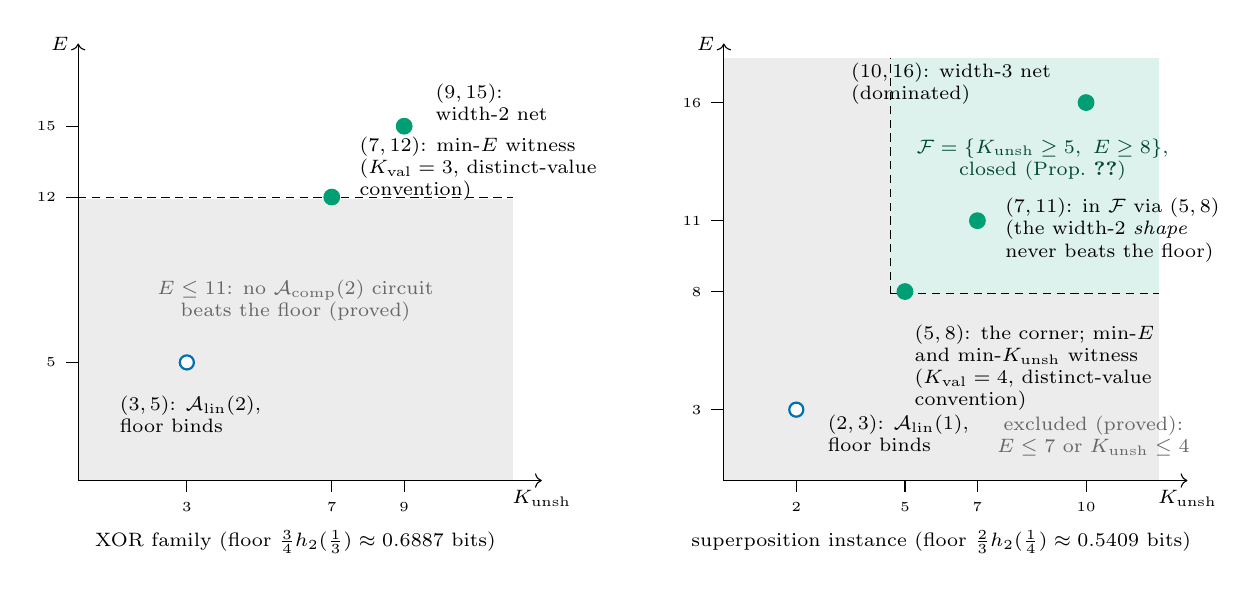
\begin{tikzpicture}[x=0.46cm, y=0.30cm,
  inF/.style={circle, draw=okgreen, fill=okgreen, inner sep=2.0pt},
  notinF/.style={circle, draw=okblue, fill=white, thick, inner sep=1.8pt},
  ptlab/.style={font=\scriptsize, align=left},
  note/.style={font=\scriptsize, align=center},
  tick/.style={font=\tiny}]
% ---------------- XOR family ----------------
\begin{scope}
\fill[gray!15] (0,0) rectangle (12.0,11.9);
\draw[->] (0,0) -- (12.8,0) node[below, ptlab] {$\Kunsh$};
\draw[->] (0,0) -- (0,18.5) node[left, ptlab] {$E$};
\foreach \k in {3,7,9}{
  \draw (\k,0) -- (\k,-0.5) node[below, tick] {$\k$};}
\foreach \e in {5,12,15}{
  \draw (0,\e) -- (-0.35,\e) node[left, tick] {$\e$};}
\draw[densely dashed] (0,12) -- (12.0,12);
\node[note, gray!80!black] at (6.0,7.6)
  {$E \le 11$: no $\cA_{\mathrm{comp}}(2)$ circuit\\
   beats the floor (proved)};
\node[notinF] at (3,5) {};
\node[ptlab, anchor=north] at (3.1,4.0)
  {$(3,5)$: $\Alin(2)$,\\ floor binds};
\node[inF] at (7,12) {};
\node[ptlab, anchor=west] at (7.5,13.2)
  {$(7,12)$: min-$E$ witness\\ ($\Kval = 3$, distinct-value\\
   convention)};
\node[inF] at (9,15) {};
\node[ptlab, anchor=west] at (9.6,16.0)
  {$(9,15)$:\\ width-2 net};
\node[note] at (6.0,-2.6) {XOR family
  (floor $\tfrac34 h_2(\tfrac13) \approx 0.6887$ bits)};
\end{scope}
% ---------------- superposition family ----------------
\begin{scope}[xshift=8.2cm]
% excluded budgets (proved): E <= 7, or K <= 4
\fill[gray!15] (0,0) rectangle (12.0,7.9);
\fill[gray!15] (0,7.9) rectangle (4.6,17.9);
% the closed frontier F = {K >= 5, E >= 8}
\fill[okgreen!13] (4.6,7.9) rectangle (12.0,17.9);
\draw[densely dashed] (4.6,7.9) -- (12.0,7.9);
\draw[densely dashed] (4.6,7.9) -- (4.6,17.9);
\draw[->] (0,0) -- (12.8,0) node[below, ptlab] {$\Kunsh$};
\draw[->] (0,0) -- (0,18.5) node[left, ptlab] {$E$};
\foreach \k in {2,5,7,10}{
  \draw (\k,0) -- (\k,-0.5) node[below, tick] {$\k$};}
\foreach \e in {3,8,11,16}{
  \draw (0,\e) -- (-0.35,\e) node[left, tick] {$\e$};}
\node[notinF] at (2,3) {};
\node[ptlab, anchor=west] at (2.6,2.0)
  {$(2,3)$: $\Alin(1)$,\\ floor binds};
\node[inF] at (5,8) {};
\node[ptlab, anchor=north west] at (5.0,7.0)
  {$(5,8)$: the corner; min-$E$\\
   and min-$\Kunsh$ witness\\
   ($\Kval = 4$, distinct-value\\
   convention)};
\node[inF] at (7,11) {};
\node[ptlab, anchor=west] at (7.5,10.6)
  {$(7,11)$: in $\cF$ via $(5,8)$\\
   (the width-2 \emph{shape}\\
   never beats the floor)};
\node[inF] at (10,16) {};
\node[ptlab, anchor=east] at (9.3,16.8)
  {$(10,16)$: width-3 net\\ (dominated)};
\node[note, gray!80!black] at (10.2,1.9)
  {excluded (proved):\\ $E \le 7$ or $\Kunsh \le 4$};
\node[note, okgreen!45!black] at (8.8,13.6)
  {$\cF = \{\Kunsh \ge 5,\ E \ge 8\}$,\\ closed
   (Prop.~\ref{prop:frontier-sup})};
\node[note] at (6.0,-2.6) {superposition instance
  (floor $\tfrac23 h_2(\tfrac14) \approx 0.5409$ bits)};
\end{scope}
\end{tikzpicture}
\caption{The payment frontier (Definition~\ref{def:frontier}), one
panel per family; axes are unshared stored-parameter counts $\Kunsh$
(Section~\ref{sec:ke-conventions}) and per-evaluation operations $E$
under the
Section~\ref{sec:classes} conventions; the parenthetical $\Kval$ notes
report the same witnesses under the different, distinct-value
convention. Filled circles: budgets at which
an affine-threshold composition provably beats the linear floor to
$H = 0$ (Thm.~\ref{thm:xor-gap}, Props.~\ref{prop:minE}
and \ref{prop:minE-sup}, Thm.~\ref{thm:superposition}(iv)); open
circles: budgets at which the
floor provably binds (Prop.~\ref{prop:budget-trivial}). Left: for XOR
the shaded region $E \le 11$ is exhaustively
excluded and the minimal-$E$ edge sits exactly at $E = 12$
(Prop.~\ref{prop:minE}); the $E = 15$ point is the hidden-layer
threshold-ladder witness, the $E = 12$ point cheaper because
$\cA_{\mathrm{comp}}(2)$ allows the second gate to read both raw
coordinates and the earlier gate's output
(Remark~\ref{rem:family-disambig}); the $\Kunsh$ structure off the
known points belongs to the residue (Open
Problem~\ref{op:frontier}(i)). Right: the superposition panel is
closed (Prop.~\ref{prop:frontier-sup}): the frontier is exactly the
quadrant $\cF = \{\Kunsh \ge 5,\ E \ge 8\}$, its corner attained by the
Prop.~\ref{prop:minE-sup} witness, every budget outside it excluded,
and the budget point $(7,11)$ in $\cF$ even though the width-2 network
shape priced there never beats the floor
(Thm.~\ref{thm:superposition}(iii), Remark~\ref{rem:budget-correction}).}
\label{fig:frontier}
\end{figure*}

Within affine-threshold compositions, floors are governed by the
partition geometry of hyperplane (or cut-point) arrangements, and a
$K$/$E$ budget translates into a counted bound on achievable cells
(intervals on the line, with skip connections amplifying them at
exactly the Lemma~\ref{lem:breakpoint} rate), which is what makes
the floors and
Propositions~\ref{prop:budget-trivial}--\ref{prop:frontier-sup}
provable; outside the class, Propositions~\ref{prop:quadratic} and
\ref{prop:sine} show that no statement of this shape survives at all.
The narrowed statement is where the theorem actually lives: at the
linear budget as accounting, at the frontier as breakpoint geometry,
with the open mathematics concentrated in the residue
(Open Problem~\ref{op:frontier}).

\section{Experiments}
\label{sec:experiments}

Three experiments test the theory where ground truth is exact, then
carry the central finding to real images and learned representations.
Experiment~1 (Section~\ref{sec:exp1}) is the protocol's analytic
calibration: a constructed Gaussian channel on which every prediction
is exactly computable, and on which the masking signature is first
exhibited. Experiment~2 (Section~\ref{sec:exp2}) demonstrates the
floor/ladder accounting empirically: trained readouts land on their
exactly computed floors, and the only readout that beats a floor pays
the counted price. Experiment~3 (Section~\ref{sec:exp3}) is the
headline: the masking signature survives real images and end-to-end
learning. Per-experiment full tables and secondary observations are
in Appendix~\ref{app:expdetails}.

\paragraph{How the claims were protected.} For each experiment, the
generative construction, seeds, training recipes, analytic
predictions, and pass/fail thresholds with tolerances were committed
to a version-controlled archive before any run; each analysis ran
exactly once on the committed protocol; and every outcome is reported,
including a failed prediction (Section~\ref{sec:exp3-cannibal}) and a
criterion that passed its point estimates but is graded inconclusive
by its own statistical-power provision (Appendix~\ref{app:protocol}).
Experiments~1 and 2 ran with no changes to their committed protocols;
in Experiment~3 one validation step in the committed protocol was
corrected before any outcome was computed (Appendix~\ref{app:protocol}).
Where a results table cites a criterion by its short archive label
(Table~\ref{tab:e3-gates}), the row also states in words what the
criterion required. The full protocol, criterion wordings, and
amendment record are in Appendix~\ref{app:protocol}; per-experiment
measurement details (estimator-bias accounting, fold schemes,
measurement-quality checks) are in Appendix~\ref{app:details}.

\subsection{Experiment 1: analytic calibration on a constructed
channel}
\label{sec:exp1}

Experiment~1's role is calibration: every quantity the protocol
measures is exactly computable from the construction, so the
estimators, tolerances, and frozen-readout shift protocol are
validated against analytic ground truth before anything is measured
where ground truth is unavailable. The masking signature is also
first exhibited here in its cleanest form.

\paragraph{Setup and protocol.} A four-dimensional Gaussian signal
$S \sim \mathcal N(0, I_4)$ drives a binary task,
$Y \mid S \sim \mathrm{Bernoulli}(\sigma(w \cdot S))$ with fixed
$w = (1,1,1,1)$; writing $u = w \cdot S / \|w\| \sim \mathcal N(0,1)$,
the task logit is $2u$. Alongside ride $\dn \in \{0, 8, 64, 256\}$
nuisance coordinates, each correlated with the signal but causally
useless ($N_j = \rho u + \sqrt{1 - \rho^2}\, \varepsilon_j$ with
$\varepsilon_j \sim \mathcal N(0,1)$ i.i.d.,
$\rho_{\mathrm{train}} = 0.9$); the shift flips the coupling sign,
$\rho_{\mathrm{shift}} = -0.9$, leaving every marginal unchanged.
Three representations are compared: the full input $X$; the lawful
compression $S$ (sufficient by construction); and the insufficient
compression $N$ (non-sufficient by construction, since
$\operatorname{Var}(u \mid N) > 0$ exactly). The readout is logistic
regression trained by damped Newton (fixed recipe), 10 seeds,
$n_{\mathrm{train}} = 50{,}000$, $n_{\mathrm{test}} = 100{,}000$;
every cross-entropy is measured out-of-sample. The analytic value of
every in-distribution cross-entropy (Gauss--Hermite quadrature), the
post-shift predictions for the frozen readout, and the seed-mean
tolerance ($0.010$ bits, sized to the predicted estimator bias;
Appendix~\ref{app:details}) were committed before any sample was
drawn; the analysis ran once; all cells are reported. For the $X$ and
$S$ arms the task is logistic-linear by construction, so
$\CE^{\star}_{\cA} = H(Y \mid Z)$ exactly. Post-shift measurements
estimate no entropy and are reported as $\CEhat_Q(\rP)$
(Definition~\ref{def:ceq}).

\paragraph{Calibration outcome: measured equals predicted.} All five
committed criteria passed; the full per-cell table is
Table~\ref{tab:e1-id} (Appendix~\ref{app:expdetails}). Lawful
compression was measured to be free: the compressed arm $S$ matched
the full arm $X$ within $+0.00000$ to $+0.00395$ bits across
$\dn = 0$--$256$ (an order of magnitude or more inside the
tolerance), at counted reductions of up to $57.9\times$ in
parameters ($521 \to 9$), $1397\times$ in training FLOPs, and
$35\times$ in inference FLOPs, with measured training FLOPs equal to
the committed formula values exactly. By
Corollary~\ref{cor:accounting} in its sign-robust form, the
substitution $X \to S$ strictly reduces $K + H_\cT + \lamvar E$ for
every $\lamvar \ge 0$; no multiplier value was used or tuned. And the
measurement landed on analytic ground truth: every (arm, $\dn$)
cell's measured $\CEhat_{\mathrm{ID}}$ fell within $0.0035$ bits of
its committed analytic value, the worst deviations matching the
predicted maximum-likelihood bias ($0.0038$ bits) almost exactly. The
estimator's measured bias is the predicted bias, which is what
licenses the same estimator and tolerances at scale.

\paragraph{The masking signature, first exhibition.} The insufficient arm
carries the finding (Table~\ref{tab:e1-shift}). The construction makes
the $N$ arm's insufficiency \emph{analytically} nearly invisible
in-distribution at large $\dn$: the true excess
$H(Y \mid N) - H(Y \mid S)$ is $0.0123$, $0.0016$, $0.0004$ bits at
$\dn = 8, 64, 256$ (the latter two below the proxy resolution
$\delta$), and the measured excesses track these values (as
pre-registered, no measured in-distribution strict-increase claim is
made at $\dn \ge 64$). Under the committed sign-flip shift, the frozen
readout's transfer cross-entropy $\CEhat_Q(\rP)$ on the same arm
degrades by $1.6666$, $1.7311$, $1.7555$ bits relative to its
in-distribution value, landing within $0.0048$, $0.0051$, $0.0140$
bits of the analytic predictions committed before the run; the lawful
arm, required to be invariant under the same shift, moved at most
$0.002$ bits at every $\dn$. Figure~\ref{fig:exp1-shift} shows the
asymmetry at a glance: the insufficient arm's in-distribution excess
and the lawful arm's post-shift drift are pinned to the axis, while
the same insufficient arm's post-shift elevation of $\CEQ{\rP}$
towers at $\approx 1.7$ bits, above the $1$-bit line that no
entropy difference on a binary task can cross.

\begin{figure}[t]
\centering
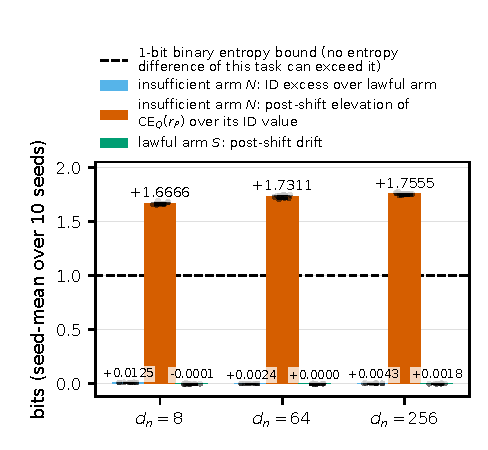
\includegraphics[width=\columnwidth]{fig_exp1_shift}
\caption{Experiment 1 headline result, computed from the committed raw
per-seed results file: for each $\dn$, the insufficient arm's
in-distribution excess held-out cross-entropy over the lawful arm
(left bars, near zero: the masking), the same arm's post-shift
elevation of the frozen-readout transfer cross-entropy $\CEQ{\rP}$ over
its own in-distribution value (center bars, $\approx 1.7$ bits), and
the lawful arm's post-shift drift (right bars, near zero). Bars are
seed-means over the 10 paired seeds, whiskers one cross-seed standard
deviation, dots the per-seed values. The dashed line marks the $1$-bit
binary entropy bound: the elevation exceeds it because $\CEQ{\rP}$ is
the cross-entropy of a $P$-fit interface under $Q$
(Definition~\ref{def:ceq}), not an entropy.}
\label{fig:exp1-shift}
\end{figure}

What kind of quantity is the $1.7$-bit degradation? It is \emph{not} a
conditional entropy: the post-shift values ($2.34$--$2.43$ bits) exceed
the $1$-bit entropy bound of a binary task, which is possible precisely
because $\CEQ{\rP}$ is the cross-entropy of a $P$-fit readout under $Q$
(Definition~\ref{def:ceq}), not an entropy. Nor is it information loss:
the sign flip $\rho \mapsto -\rho$ leaves every marginal (and
$I(N; Y)$) essentially unchanged, and a readout \emph{retrained
under $Q$} would land back at the in-distribution numbers, showing
none of the degradation. The $1.7$ bits is frozen-readout
\textbf{transfer risk}: the $P$-fit interface points the wrong way
under $Q$. An insufficiency whose in-distribution footprint is
$0.0004$ bits (unmeasurable under any realistic tolerance) thus
manifests as deployment brittleness that is structurally invisible to
any in-distribution evaluation and to any evaluation that is allowed
to refit; an audit that evaluates only in-distribution, or that
silently refits, can certify a representation carrying an arbitrarily
large latent deployment liability. The committed failure conditions
did not occur at any cell, and the committed measurement-quality
checks all passed; pre-declared secondary observations (including the
raw $X$ arm's own drift under shift) are in
Appendix~\ref{app:expdetails}.

\begin{table}[t]
\centering
\caption{Experiment 1, shift protocol: pre-registered prediction vs.\
measurement (seed-means, 10 seeds, bits). Post-shift values are
frozen-readout transfer cross-entropies $\CEhat_Q(\rP)$
(Definition~\ref{def:ceq}), not conditional entropies; they may and do
exceed the $1$-bit binary entropy bound. ``Lawful drift'' is
$\overline{\CEhat}_{\mathrm{shift}}(S) - \overline{\CEhat}_{\mathrm{ID}}(S)$;
the analytic in-distribution excess of the insufficient arm over the lawful arm
is shown for the masking comparison.}
\label{tab:e1-shift}
\footnotesize
\setlength{\tabcolsep}{2.6pt}
\begin{tabular}{lrrrrrr}
\toprule
& \multicolumn{2}{c}{ID excess, $N$ arm} &
\multicolumn{3}{c}{$\CEhat_Q(\rP)$, $N$ arm} & lawful drift \\
\cmidrule(lr){2-3}\cmidrule(lr){4-6}
$\dn$ & analytic & meas. & pred. & meas. & $|$dev.$|$ & meas. \\
\midrule
8 & 0.0123 & $+0.0125$ & 2.3414 & 2.3463 & 0.0048 & $-0.00012$ \\
64 & 0.0016 & $+0.0024$ & 2.4047 & 2.3996 & 0.0051 & $+0.00003$ \\
256 & 0.0004 & $+0.0043$ & 2.4118 & 2.4259 & 0.0140 & $+0.00184$ \\
\bottomrule
\end{tabular}
\end{table}

\subsection{Experiment 2: the readout ladder}
\label{sec:exp2}

\paragraph{Setup and protocol.} The construction is a scaled-up
sibling of the superposition family of
Section~\ref{sec:superposition}. A feature vector $F$ is uniform on
the $\binom{16}{4} = 1820$ binary patterns with exactly $k = 4$ of
$\dfeat = 16$ features active; a fixed per-seed Gaussian projection
superposes them, $Z = AF$, noiseless; the task reads one feature,
$Y = F_1$. Atom injectivity was verified per cell before the run, so
$H(Y \mid Z) = 0$ \emph{exactly} everywhere: every bit of measured
uncertainty is interface-induced. Superposition load
$\dfeat / \dz = 4.0$--$1.33$ across $\dz \in \{4, 6, 8, 12\}$; 10
seeds; $n_{\mathrm{train}} = 20{,}000$,
$n_{\mathrm{test}} = 100{,}000$. Three readout rungs of strictly
increasing declared cost (Table~\ref{tab:e2-ladder},
Appendix~\ref{app:expdetails}): (i) a soft linear-logistic readout,
whose population optimum is $\CE^{\star}_{\mathrm{lin}}$
(Definition~\ref{def:cestar}); (ii) a two-layer ReLU network of width
64; (iii) an oracle nearest-atom decoder over the 1820 constructed
atoms (a codebook-lookup \emph{accounting} rung, not a trained
readout). The key design choice: the linear class's floor is an
\emph{exact population quantity}, computed per seed by convex
optimization on the exact 1820-atom distribution and committed before
the run; no training budget moves a linear readout below it, which
is what makes ``equivalent-budget comparison'' exact rather than
rhetorical. Committed tolerance $0.010$ bits, with a
statistical-power provision grading any comparison whose cross-seed
standard error exceeds $0.005$ bits inconclusive; the analysis ran
once; all cells and seeds are reported.

\paragraph{Results.} All primary criteria passed
(Table~\ref{tab:e2-floors}, Appendix~\ref{app:expdetails});
Figure~\ref{fig:exp2-ladder} plots the whole experiment as prediction
against measurement. The exact floors are real, out-of-sample: the
trained linear rung reproduced its committed per-seed
$\CE^{\star}_{\mathrm{lin}}$ floor with seed-mean deviations
$+0.0013$, $-0.0001$, $+0.0000$, $+0.0002$ bits at
$\dz = 4, 6, 8, 12$. Beating a floor carried the counted price: at
the declared gap cells $\dz \in \{4, 6, 8\}$ the oracle rung achieved
$1.44 \times 10^{-6}$ bits (exactly the pre-registered
probability-clip artifact; decode accuracy 1.0), beating the exact
linear floors by $0.6053$, $0.4799$, $0.3196$ bits (below a floor
no training budget within the linear class can cross), carried by a
rung whose counted $K$ is $1820\times$ larger and whose counted
inference cost is $1577$--$1978\times$ larger. (The oracle rung
proves that zero task uncertainty is \emph{available} given codebook
storage and search; it does not prove that ordinary training finds it
cheaply.) The accounting held everywhere: $K$ and $E$ strictly
increase up-ladder at all 40 cells exactly as committed
(Proposition~\ref{prop:ladder}), and the committed failure condition
(a readout at linear $K$/$E$ measuring below the exact linear
floor by more than the tolerance) did not occur at any cell or
seed. At $\dz = 12$, where 5 of 10 seeds are linearly separable
(floor $\approx 0$), rungs (i) and (ii) both sit at their floors: no
superposition pressure, no gap, the data-side analogue of the
equality rung of Theorem~\ref{thm:superposition}(iii). No measured
quantity here estimates a hard-class $H_{\cA}$: the theorem-side hard
floors of Theorem~\ref{thm:superposition} and the experiment-side
soft floors are different objects, each computed exactly in its own
way.

\begin{figure}[t]
\centering
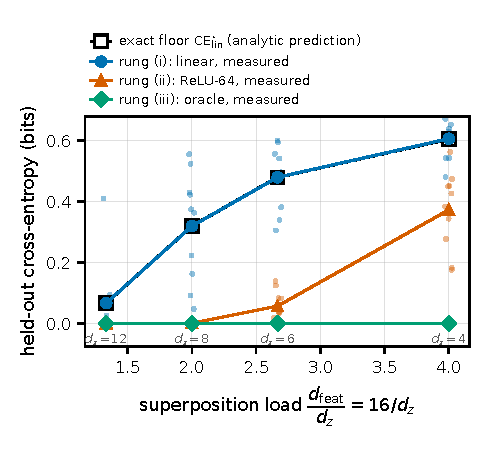
\includegraphics[width=\columnwidth]{fig_exp2_ladder}
\caption{Experiment 2 ladder, computed from the committed raw per-seed
results file: measured held-out cross-entropy of the three rungs versus
superposition load $\dfeat / \dz$, with the exact per-seed population
floors $\CE^{\star}_{\mathrm{lin}}$ (computed by convex optimization and
committed before the run; the file's \texttt{analytic\_floor} column)
overlaid as the dashed prediction line. Solid markers are seed-means
over 10 seeds; faint dots are the per-seed values, whose vertical spread
is real cross-projection heterogeneity (each seed draws its own $A$),
not measurement noise. The measured linear rung is visually
indistinguishable from its committed floor (worst seed-mean deviation
$0.0013$ bits); the oracle rung sits at the clip artifact
$1.44 \times 10^{-6}$ bits at every load.}
\label{fig:exp2-ladder}
\end{figure}

A committed secondary criterion (whether the \emph{trained}
width-64 network beats the exact linear floor by pre-set margins)
passed its point estimates at both declared cells, yet is reported
inconclusive because the registration's own statistical-power
provision binds; the full episode, a worked example of the protocol
applied against the experimenters' reading of the evidence, is in
Appendix~\ref{app:protocol-e23}. Measurement-quality checks and one
infrastructure disclosure are in Appendix~\ref{app:details}.

\subsection{Experiment 3: masking at scale}
\label{sec:exp3}

Experiments~1 and 2 run where ground truth is analytic; Experiment~3
scales the masking finding to real images and \emph{learned}
representations, with the construction retreating to the one place it
is still needed: the spurious coupling itself. The question,
committed before any run: does the masking signature (a
cue-reliant representation indistinguishable from or better than a
sufficient one in-distribution, whose frozen interface collapses
under a coupling-breaking shift) reproduce when the representation
is a CNN trained end-to-end on CIFAR-10?

\paragraph{Setup.} Every train, test, and shift image set is built by
one pinned construction module and no other code
(Appendix~\ref{app:details}). CIFAR-10 ($50{,}000$ train / $10{,}000$
test, $|\cY| = 10$ exactly uniform, so
$H(Y) = \log_2 10 \approx 3.3219$ bits); per image, an indicator
$s \in \{0, \dots, 9\}$ drawn with $P(s = y) = \rho$ (off-diagonal
uniform), and a per-class chromatic tint (ten maximally separated
zero-mean hues, distinct, hence injective in $s$) added at fixed
strength $0.20$ (Figure~\ref{fig:exp3-stimuli}). Two arms differ
\emph{only} in the coupling: the
\textbf{naive} arm trains at $\rho \in \{0.7, 0.9, 0.95, 0.99\}$ (the
tint is informative about $y$ only through the train-time coupling:
a spurious-cue condition by construction); the \textbf{lawful} arm (the
cue-decorrelated control) trains
decorrelated at $\rho_{\mathrm{eff}} = 1/|\cY| = 0.1$, the no-coupling
fixed point: the tint is present with identical marginal statistics
but carries zero \emph{population} label information, so it adds no task
information any readout can use (a finite-sample model may still encode
the independent nuisance, but cannot gain label information from it).
Shifts re-draw only the indicator, leaving image
content untouched: \emph{decorrelate} ($s$ uniform, independent of
$y$; the primary shift, the marginal-controlled cue-breaking analogue
of Experiment~1's sign flip) and \emph{anticorrelate} ($s = y$ with
probability $1 - \rho$; descriptive only, reported in full). At
$\rho = 0.9$ the two shift distributions coincide, a fact the
registration turns into a free pipeline-consistency check
(Table~\ref{tab:e3-gates}, last row). Model:
a 9-block CNN ($1{,}739{,}210$ parameters), $30$ epochs, fixed recipe;
$10$ seeds $\times$ $4$ coupling cells $\times$ $2$ arms $= 80$
training runs, all seeds committed in advance. Representation $Z$: the
$256$-dimensional penultimate features. Readout: multinomial logistic
regression on $Z$ ($K_{\mathrm{readout}} = 10 \times 257 = 2570$), fit
on one stratified half of the test pool ($5{,}000$) and evaluated
held-out on the other ($5{,}000$); the frozen readout is never
evaluated on re-tinted versions of images it was fit on. Per cell,
three measurements ($\CEhat_{\mathrm{ID}}$, the frozen
$\CEhat_Q(\rP)$, and a $5$-fold $Q$-refit
$\CEhat_{Q\text{-refit}}$) yield the two differences the criteria
consume:
\begin{gather*}
\Delta_{\mathrm{info}} := \CEhat_{Q\text{-refit}} - \CEhat_{\mathrm{ID}},
\\
\Delta_{\mathrm{transfer}} := \CEhat_Q(\rP) - \CEhat_{Q\text{-refit}},
\end{gather*}
the first estimating the change in the class's population optimum,
$\CE^{\star}_{\cA}(Q) - \CE^{\star}_{\cA}(P)$
(Definition~\ref{def:cestar}), the information accessibility lost
under shift, and the second the transfer risk of the frozen interface
(Definition~\ref{def:ceq}): exactly the decomposition the four-quantity
vocabulary of Section~\ref{sec:three-quantities} exists to keep
separate.

\begin{figure}[t]
\centering
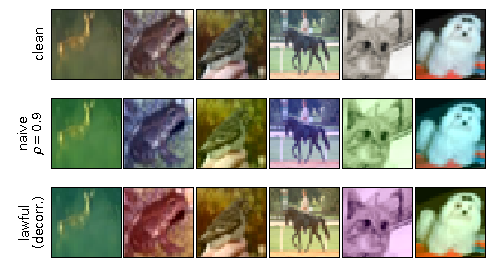
\includegraphics[width=\columnwidth]{fig_exp3_stimuli}
\caption{Experiment 3 stimuli, built by the pinned construction module
(SHA-256 in Appendix~\ref{app:details-e3}) from CIFAR-10 test images
(fixed-seed selection, six classes). Top row: clean originals. Middle
row: the naive arm's view at $\rho = 0.9$; the additive class-indexed
chromatic tint (strength $0.20$) is the \emph{entire} manipulation,
and its indicator agrees with the true label with probability $\rho$.
Bottom row: the lawful (control) arm's view, which receives the same
tint marginal with the indicator drawn independently of the label, so
the identical manipulation carries zero label information.}
\label{fig:exp3-stimuli}
\end{figure}

\paragraph{Protocol.} The construction pins, training recipe, readout
class, seed list, criteria, and thresholds (per-cell tolerance
$\delta_{\mathrm{cell}} = \max(2 \times SE_{\mathrm{seed}},\ 0.10\
\text{bits})$, with a statistical-power clause) were committed before
any naive arm was trained or any shift set built, and the committed
analysis script ran exactly once. One validation step (a selftest
of the cross-entropy estimator against planted ground truth) was
found by its own committed check to validate the wrong estimand and
was corrected before any outcome was unblinded, the single dated
amendment the registered policy permits (full record, including the
preserved failure: Appendix~\ref{app:protocol-amend}). One
consequence carries to every number below: at this readout dimension
the absolute held-out cross-entropy is not a validated estimator of
the population optimum, while the cross-entropy \emph{differences}
the criteria consume ($\Delta_{\mathrm{info}}$,
$\Delta_{\mathrm{transfer}}$, and between-arm gaps) are recovered to
the stated tolerance. Absolute values are therefore reported as raw
descriptive losses, and pass/fail claims rest only on validated
differences.

\paragraph{Results.} All five committed criteria pass
(Table~\ref{tab:e3-gates}); the verdict rule committed in the
registration (all four pass/fail criteria must pass) is met, so
the masking signature is \emph{reproduced at scale}. An independent
confirmatory re-run --- a fresh $80$-cell sweep across all four couplings on
separate hardware --- reproduces the committed seed-means within $\epsilon$
(gate-level $\epsilon \le 0.05$ bits, $0.026$ bits on the gated decorrelate
cell; per-cell $\le 0.31$ bits), every gate verdict unchanged.
The gates are evaluated on seed-means with a normal-SE slack; two
assumption-light per-seed checks corroborate the headline brittleness
claim (G-B2) without that bound. An exact sign test that the naive arm's
per-seed $\Delta_{\mathrm{transfer}}$ clears the committed $0.5$-bit
threshold passes at every gated coupling ($9/10$ seeds at $\rho = 0.9$,
$p = 0.011$; $10/10$ at $\rho \in \{0.95, 0.99\}$, $p = 0.00098$, the
exact $n = 10$ floor), and an exact paired permutation test of
naive-minus-lawful $\Delta_{\mathrm{transfer}}$ rejects at the $n = 10$
two-sided floor $p = 2/2^{10} = 0.0020$ at all three couplings
(reproduced by \texttt{paired\_tests.py} in the Experiment~3
directory of the reproduction repository~\cite{porepro}).
Table~\ref{tab:e3-cells} gives the
naive arm's cell means under the primary shift and
Figure~\ref{fig:exp3-masking} the masking curve, computed from the
committed per-seed results file.

\begin{table*}[t]
\centering
\caption{Experiment 3: the five pre-registered criteria, committed
threshold against measurement (bits, seed-means over all 10 seeds;
decorrelate shift). Archive labels in parentheses
(Table~\ref{tab:artifacts}). $\delta$ is the committed per-cell formula
$\max(2 \times SE_{\mathrm{seed}}, 0.10)$; the $0.10$-bit floor bound
everywhere except the naive $\rho = 0.99$ transfer cell
($\delta = 0.1177$), far inside the $0.25$-bit underpowered trigger,
which never fired.}
\label{tab:e3-gates}
\footnotesize
\setlength{\tabcolsep}{4.0pt}
\begin{tabular}{@{}p{3.55cm}p{5.55cm}p{4.85cm}l@{}}
\toprule
criterion & committed threshold & measured & verdict \\
\midrule
E3.1 (\texttt{G-B1}) masking-ID premise &
naive$\,-\,$lawful $\CEhat_{\mathrm{ID}} \le +\delta$ at every $\rho$ &
$-0.1017$ / $-0.1901$ / $-0.2295$ / $-0.3018$ & \textbf{PASS} \\
E3.2 (\texttt{G-B2}) naive transfer brittleness &
$\Delta_{\mathrm{transfer}} \ge 0.5$ bits at each
$\rho \in \{0.9, 0.95, 0.99\}$ &
$0.5524$ / $1.0985$ / $3.5603$ & \textbf{PASS} \\
E3.3 (\texttt{G-B3}) lawful arm flat &
lawful $|\Delta_{\mathrm{info}}|, |\Delta_{\mathrm{transfer}}| \le \delta$
at every $\rho$ & largest deviation $0.0206$, both shifts & \textbf{PASS} \\
E3.4 (\texttt{G-B4}) masking-curve monotonicity &
$\Delta_{\mathrm{transfer}}$ non-decreasing in $\rho$ (slack $\delta$) &
$0.1020 < 0.5524 < 1.0985 < 3.5603$, strict & \textbf{PASS} \\
E3.5 (\texttt{C-B5}) $\rho = 0.9$ coincidence &
dec/anti frozen $\CEhat_Q(\rP)$ agree within $\delta$ (validity check) &
$0.0014$ (naive), $0.0050$ (lawful) & consistent \\
\bottomrule
\end{tabular}
\end{table*}

\begin{table}[t]
\centering
\caption{Experiment 3, naive arm under the primary decorrelate shift
(bits, seed-means over 10 seeds; cross-seed SEs $0.0035$--$0.0588$).
$\CEhat$ columns are raw descriptive held-out losses: at this
readout dimension the absolute held-out cross-entropy is not a
validated estimator of the population optimum, and pass/fail claims
rest only on the validated differences (Section~\ref{sec:exp3});
$\CEhat_Q(\rP)$ is the frozen transfer cross-entropy
(Definition~\ref{def:ceq}). The lawful arm's corresponding
$\CEhat_{\mathrm{ID}}$ is $0.4102$--$0.4190$ across cells with
$|\Delta_{\mathrm{info}}|, |\Delta_{\mathrm{transfer}}| \le 0.0206$
everywhere, both shifts.}
\label{tab:e3-cells}
\footnotesize
\setlength{\tabcolsep}{3.4pt}
\begin{tabular}{lrrrr}
\toprule
$\rho$ & $\CEhat_{\mathrm{ID}}$ & $\CEhat_Q(\rP)$ &
$\Delta_{\mathrm{info}}$ & $\Delta_{\mathrm{transfer}}$ \\
\midrule
0.70 & 0.3154 & 0.6685 & 0.2511 & 0.1020 \\
0.90 & 0.2266 & 1.2874 & 0.5084 & 0.5524 \\
0.95 & 0.1807 & 1.9646 & 0.6854 & 1.0985 \\
0.99 & 0.1172 & \textbf{4.7737} & 1.0962 & \textbf{3.5603} \\
\bottomrule
\end{tabular}
\end{table}

\begin{figure}[t]
\centering
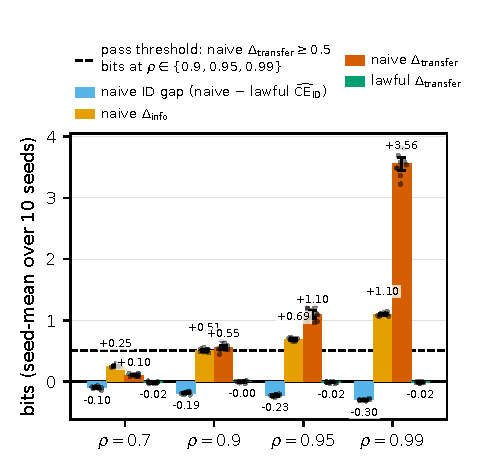
\includegraphics[width=\columnwidth]{fig_exp3_masking}
\caption{Experiment 3 masking curve, computed from the committed
per-seed results file (no measured value is transcribed by hand): for
each train-time coupling $\rho$, the naive arm's in-distribution gap to
the lawful arm (negative bars: the insufficient arm is \emph{rewarded}
in-distribution), the naive arm's $\Delta_{\mathrm{info}}$ and
$\Delta_{\mathrm{transfer}}$ under the primary decorrelating shift, and
the lawful arm's $\Delta_{\mathrm{transfer}}$ (flat). Bars are
seed-means over the 10 paired seeds; whiskers are 2000-resample
bootstrap 95\% CIs of the seed-mean; dots are per-seed values. The
dashed line is the committed $0.5$-bit transfer-brittleness threshold
(criterion E3.2, Table~\ref{tab:e3-gates}).}
\label{fig:exp3-masking}
\end{figure}

Three readings of the table and figure.
\emph{First, the masking premise holds in its amplified form.}
In-distribution, the naive arm is \emph{better} than the lawful arm
at every coupling, by a margin growing to $-0.30$ bits
at $\rho = 0.99$, where the committed construction arithmetic (the
cue-only anchor against the realized lawful floor) put the expected gap
at $\approx -0.31$: the measured value lands within $0.005$ bits of the
construction's own expectation. In-distribution evaluation rewards
the insufficiency rather than exposing it.
\emph{Second, the collapse under shift is large, graded, and
interface-borne at the top.} The frozen interface's
$\Delta_{\mathrm{transfer}}$ rises strictly ($0.1020$, $0.5524$,
$1.0985$, $3.5603$ bits; 95\% CIs $[0.091, 0.115]$, $[0.518, 0.590]$,
$[1.036, 1.156]$, $[3.448, 3.669]$), while the lawful arm's worst
deviation anywhere, either shift, is $0.0206$ bits. At $\rho = 0.99$
the frozen $\CEhat_Q(\rP)$ reaches $4.7737$ bits ($5.2748$ under the
descriptive anticorrelate shift), above the $\log_2 10 = 3.3219$-bit
ten-class entropy bound, which is the Section~\ref{sec:three-quantities}
tell that this number is a property of the fitted interface (quantity
$\CEQ{\rP}$), not an entropy of anything. As a fraction of the
committed cue-only envelope (the closed-form collapse of an idealized
calibrated cue reader), the trained system realizes
$f(\rho) = 0.1089$, $0.1742$, $0.4082$ at $\rho = 0.9, 0.95, 0.99$:
inside the committed band $[0.1, 1]$ at every point, grazing its lower
edge at $\rho = 0.9$. \emph{Third, the validity checks held.} The
$\rho = 0.9$ coincidence check agreed at the millibit level
($0.0014$ and $0.0050$ bits); every readout fit converged; and the
lawful arm's four identical-data replicate trainings per seed put CNN
training nondeterminism at $\approx 0.025$ bits mean per-seed range,
an order of magnitude inside the smallest threshold any criterion
uses, and a free calibration number for future real-data protocols
(further checks in Appendix~\ref{app:details}).

\subsubsection{Cue cannibalization: the deviation, and what it bounds}
\label{sec:exp3-cannibal}

\begin{figure}[t]
\centering
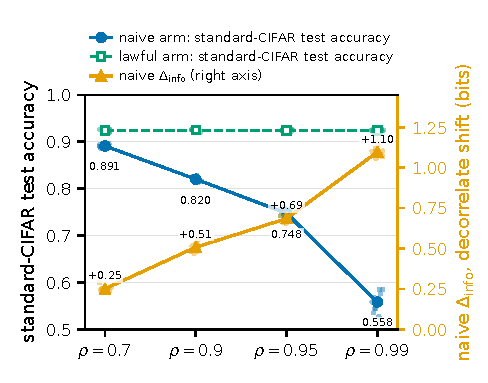
\includegraphics[width=\columnwidth]{fig_exp3_cannibal}
\caption{Cue cannibalization, computed from the committed campaign
artifacts (per-seed accuracies from the results summary, per-seed
$\Delta_{\mathrm{info}}$ from the results file; nothing transcribed by
hand): against train-time coupling $\rho$, the naive arm's accuracy on
\emph{standard, untinted} CIFAR-10 test images (left axis) falls from
$0.891$ to $0.558$ while the lawful arm stays flat at
$0.924$--$0.925$ (dashed reference), and the naive arm's
$\Delta_{\mathrm{info}}$ under the primary decorrelating shift (right
axis, bits) rises in step. Lines are seed-means over the 10 seeds,
dots per-seed values. At high coupling the cue does not ride on top of
intact image features; it \emph{displaces} image-feature learning, so
part of the shift damage is representation-borne
(Section~\ref{sec:exp3-cannibal}).}
\label{fig:exp3-cannibal}
\end{figure}

One committed prediction failed, and it is the most informative number
in the experiment. The pre-registration predicted, descriptively
(with no pass/fail threshold attached),
$\Delta_{\mathrm{transfer}} \gg \Delta_{\mathrm{info}}$ at
$\rho \ge 0.9$, ratio $\ge 2$: the collapse should be interface-borne,
not information-borne, as in Experiment~1. Measured ratios: $1.09$ at
$\rho = 0.9$, $1.60$ at $0.95$, $3.25$ at $0.99$. The prediction
fails at the two moderate couplings and holds only at the extreme one.
The mechanism is visible in a pre-registered sanity metric: the naive
arm's accuracy on \emph{standard, untinted} CIFAR-10 falls from
$0.891$ at $\rho = 0.7$ to $0.558$ at $\rho = 0.99$ (lawful:
$0.924$--$0.925$ everywhere; Figure~\ref{fig:exp3-cannibal}). The
naive CNN does not add a cue route on
top of intact image features; it \emph{cannibalizes} image-feature
learning, so that under shift even a refit readout finds less
accessible label information in $Z$:
$\Delta_{\mathrm{info}}$ reaches $1.0962$ bits at $\rho = 0.99$,
within its committed bound (the cue's genuine in-distribution
information value, $3.2094$ bits there) but not small. This deviation
\emph{bounds} the paper's interface-borne story, and the text should
say so plainly: the direction survives everywhere the prediction
applied ($\Delta_{\mathrm{transfer}} > \Delta_{\mathrm{info}}$ at
every $\rho \ge 0.9$), but the quantitative form ``brittleness is interface-borne,
not information-borne'' is correct only at extreme coupling; at
moderate coupling the collapse splits between interface brittleness
and genuine representation damage in comparable parts. Experiment~1's
clean separation is a property of its frozen \emph{linear} readout over
a fixed representation; when the representation itself is learned
against the cue, the cue reshapes the representation too. The
decomposition that exposes this ($\Delta_{\mathrm{transfer}}$
against $\Delta_{\mathrm{info}}$, kept separate by the
Section~\ref{sec:three-quantities} vocabulary) is exactly what an
evaluation conflating the four quantities could not have reported.

Scope: one dataset, one architecture, one nuisance design, one
readout class, constructed shifts; nothing here is a claim about
natural spurious correlations (Section~\ref{sec:limitations}).

\section{Discussion}
\label{sec:discussion}

The recent turn toward observer-dependent information has two
complementary edges: how much reusable \emph{structure} a
computation-bounded learner can extract from data---measured by
epiplexity in concurrent work of Finzi et al.~\cite{finziepiplexity}---and
how much \emph{task-predictive} information a readout-bounded observer
can actually use, which is the edge this paper prices exactly
(Section~\ref{sec:related}), together with what deploying that readout
costs under distribution shift.

\paragraph{Recommendation: report frozen-versus-refit pairs.} The
paper's practical output is a reporting practice, not a theorem. For a
system whose readout is fit under one distribution and deployed where
the distribution may shift, evaluate the relevant shifts twice: once
with the deployed readout frozen, once with the readout refit under
the shifted distribution, and report the pair
(Figure~\ref{fig:frozen-refit}). The frozen number estimates the loss
of the deployed frozen interface under the specified shift; the refit
number is what the representation still supports; their difference is the price of the
readout interface, and it is invisible to any protocol that reports
only one of the two. In-distribution evaluation cannot substitute for
the pair at any sample size: in both masking experiments it did
worse than fail to expose the fragile models; it actively preferred
them.

\begin{figure}[t]
\centering
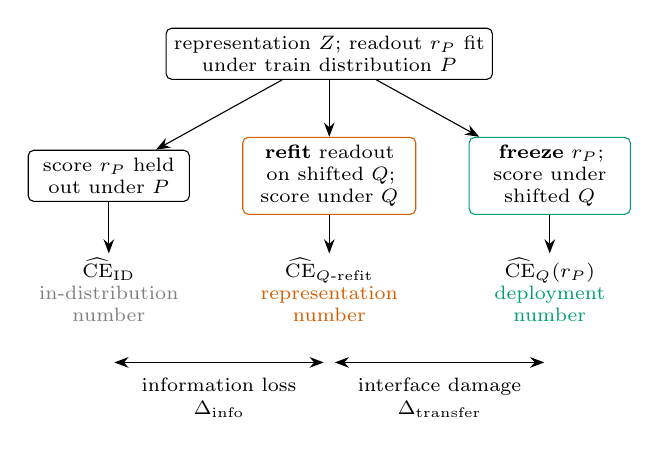
\begin{tikzpicture}[
  >={Stealth[length=1.8mm]},
  box/.style={draw, rounded corners=2pt, align=center,
    font=\scriptsize, inner sep=2.8pt},
  res/.style={align=center, font=\scriptsize, inner sep=1.5pt},
  gaplab/.style={font=\scriptsize, align=center}
]
% the shared upstream object
\node[box] (top) at (4.0,4.2)
  {representation $Z$; readout $\rP$ fit\\ under train distribution $P$};
% the three evaluations
\node[box, text width=1.85cm] (sid) at (1.2,2.65)
  {score $\rP$ held out under $P$};
\node[box, draw=okverm, text width=2.0cm] (sref) at (4.0,2.65)
  {\textbf{refit} readout on shifted $Q$;\\ score under $Q$};
\node[box, draw=okgreen, text width=1.85cm] (sfro) at (6.8,2.65)
  {\textbf{freeze} $\rP$;\\ score under shifted $Q$};
\draw[->] (top) -- (sid);
\draw[->] (top) -- (sref);
\draw[->] (top) -- (sfro);
% the three reported numbers
\node[res] (rid) at (1.2,1.2)
  {$\CEhat_{\mathrm{ID}}$\\ {\color{gray}in-distribution}\\ {\color{gray}number}};
\node[res] (rref) at (4.0,1.2)
  {$\CEhat_{Q\text{-refit}}$\\
   \textcolor{okverm}{representation}\\ \textcolor{okverm}{number}};
\node[res] (rfro) at (6.8,1.2)
  {$\CEhat_Q(\rP)$\\ \textcolor{okgreen}{deployment}\\ \textcolor{okgreen}{number}};
\draw[->] (sid) -- (rid);
\draw[->] (sref) -- (rref);
\draw[->] (sfro) -- (rfro);
% the two reported differences
\draw[<->, shorten <=2pt, shorten >=2pt] (1.2,0.28) -- (4.0,0.28);
\node[gaplab, anchor=north] at (2.6,0.20)
  {information loss\\ $\Delta_{\mathrm{info}}$};
\draw[<->, shorten <=2pt, shorten >=2pt] (4.0,0.28) -- (6.8,0.28);
\node[gaplab, anchor=north] at (5.4,0.20)
  {interface damage\\ $\Delta_{\mathrm{transfer}}$};
\end{tikzpicture}
\caption{The recommended frozen-versus-refit reporting pair. A readout
$\rP$ is fit on the representation under the training distribution $P$;
its held-out score there is the in-distribution number. For a shift of
interest $Q$, score twice: with $\rP$ \emph{frozen}, giving the
deployment number $\CEhat_Q(\rP)$, the loss the deployed interface
actually delivers under the shift; and with the readout \emph{refit}
under $Q$ on the same representation, giving the representation number
$\CEhat_{Q\text{-refit}}$, the best the representation still supports
for that readout class. The pair separates the two failure modes that
single-number evaluation conflates: frozen $-$ refit
($\Delta_{\mathrm{transfer}}$) is interface damage, the fitted readout
no longer matching the shifted data; refit $-$ ID
($\Delta_{\mathrm{info}}$) is information loss, a genuine change in the
label information the class can access in the representation.}
\label{fig:frozen-refit}
\end{figure}

\paragraph{Why the pair is necessary.} In-distribution testing
estimates one of the four quantities of
Section~\ref{sec:three-quantities} (the best cross-entropy a soft
readout can attain under the training distribution) and estimates
it well: in every validated cell the measurement landed on its
analytic target to within the predicted estimator bias. But what
deployment experiences under shift is a different quantity, the
transfer cross-entropy of the \emph{frozen} interface, and no
in-distribution measurement bounds it. The gap between the two is not
a technicality: in the constructed channel, an insufficiency of
$0.0004$ bits became $\approx 1.7$ bits of transfer damage the moment
the nuisance--signal coupling moved; on real images, the cue-reliant
networks measured better than the control under every standard test
and collapsed only under the frozen-readout audit.

\paragraph{Interface damage and representation damage.} Experiment~3's
decomposition adds a caution that the constructed channel alone would
have missed, and it comes from this paper's one failed prediction
(Section~\ref{sec:exp3-cannibal}): at extreme coupling the collapse
is carried almost entirely by the fitted interface, as in
Experiment~1, where the representation is fixed by construction; at
moderate coupling a network trained against a strong cue also learns
less image structure, and the interface and representation damage are
comparable in size. The two components are separable by measurement
(that is what the frozen-versus-refit difference pair does), but
both are real.

\subsection{External replication on a pretrained language model}
\label{sec:pythia}

The experiments above use a constructed channel and from-scratch CIFAR
networks, where ground truth is exact. As a post-hoc external check (not
pre-registered, unlike Experiments~1--3), we ask whether the
frozen-versus-refit decomposition and the two failure modes it separates
survive on a real, off-the-shelf pretrained model: \textbf{Pythia-410m}
($\approx 300$B Pile tokens). The same head-only-refit protocol applies,
scored in bits per byte so the numbers are comparable across tokenizations;
corpus sizes, the refit optimizer and budget, the quantization procedure,
and the single-run (unaveraged) status of every cell are specified in
Appendix~\ref{app:pythia}.

\paragraph{Weight quantization is information-borne (an irreducible refit floor).}
Quantizing the weights and measuring frozen versus head-refit cross-entropy on
in-distribution text (WikiText-103) reproduces the information-borne signature:
8-bit is free, and below it a floor appears that head-refit cannot remove, with
a sharp onset between 4 and 3 bits (Table~\ref{tab:pythia-quant}; Figure~\ref{fig:pythia}a). Refitting the
head recovers a bounded fraction ($23$--$31\%$, the
interface-borne part); the remainder is irreducible information loss. On this
well-trained model the frontier is earlier and steeper than on the from-scratch
toy (which paid $0.007$ bits irrecoverable at 4-bit): trained weights use their
precision, so they tolerate quantization less --- the realistic regime.

\begin{table*}[t]
\centering\small
\begin{tabular}{r r r r r}
\hline
bits & total & recoverable (interface) & irrecoverable (info) & \% interface\\
\hline
8 & 0.021 & 0.020 & 0.001 & free\\
4 & 0.273 & 0.075 & \textbf{0.198} & 27\%\\
3 & 1.875 & 0.430 & \textbf{1.445} & 23\%\\
2 & 2.336 & 0.731 & \textbf{1.605} & 31\%\\
\hline
\end{tabular}
\caption{Weight quantization on Pythia-410m (bits/byte, in-distribution;
reference is the 16-bit head-refit score, $0.976$, fit on text disjoint from
the evaluation set). Head-refit recovers the
interface-borne part; the irrecoverable column is the information-borne floor,
with a sharp 4-to-3-bit onset.}
\label{tab:pythia-quant}
\end{table*}

\paragraph{Distribution shift is interface-borne, growing with OOD distance.}
The shift leg requires a genuinely out-of-distribution shift: code and Japanese
are \emph{in} Pythia's training mixture, so its frozen readout does not collapse
on them and head-refit recovers nothing --- the interface-borne mechanism is
invisible when the ``shift'' is in-distribution. Adding low-resource,
Pile-underrepresented languages exposes it, and the head-refit-recoverable
fraction grows monotonically with how far out-of-distribution the shift is
(frozen cross-entropy as the OOD-distance proxy): near zero for mild shifts, up
to $\approx 0.26$ bits/byte for clearly-OOD languages
(Table~\ref{tab:pythia-ood}; Figure~\ref{fig:pythia}b; Pearson $0.94$, Spearman $0.86$, $n=8$,
Latin-script). At the far end the recovered fraction is only $\approx 17\%$ of
the gap --- the body genuinely under-represents the language --- so very-OOD
shift is mixed, a real interface-borne component over a representation-borne
residual; the frozen-versus-refit pair reads off both.

\begin{table}[t]
\centering\footnotesize
\begin{tabular}{l r r}
\hline
shift & frozen (OOD-ness) & refit recovery\\
\hline
code & 0.68 & $-0.033$\\
Japanese & 1.10 & $+0.009$\\
Vietnamese & 1.24 & $+0.030$\\
Indonesian & 1.54 & $+0.043$\\
Finnish & 1.57 & $+0.011$\\
Yoruba & 2.22 & $\mathbf{+0.261}$\\
Swahili & 2.34 & $\mathbf{+0.242}$\\
Welsh & 2.46 & $\mathbf{+0.253}$\\
\hline
\end{tabular}
\caption{Distribution shift on Pythia-410m (bits/byte; refit fit on
within-domain text disjoint from the evaluation set). The
head-refit-recoverable (interface-borne) part is near zero (and, for
in-mixture code, marginally negative) for in-distribution/mild shifts and
grows to a quarter-bit for genuinely-OOD
languages; recovery tracks OOD distance (Pearson $0.94$). Same-script-width
corpora only (a multi-byte-script point is excluded as a bits-per-byte artifact).}
\label{tab:pythia-ood}
\end{table}

\begin{figure*}[t]
\centering
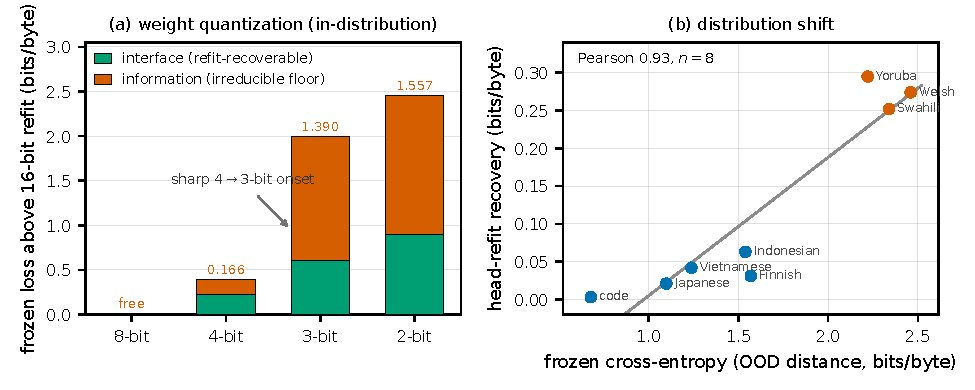
\includegraphics[width=\textwidth]{fig_pythia}
\caption{External replication on Pythia-410m (post-hoc, not
pre-registered): the two failure modes the paper isolates on systems with
exact ground truth, separated by the same frozen-versus-refit pair. \textbf{(a)} Weight quantization (in-distribution;
bits/byte above the 16-bit head-refit reference). Each bar splits the frozen
loss into the head-refit-recoverable interface part and the irreducible
information-borne floor; the floor jumps sharply between 4 and 3 bits, the
information-borne signature. \textbf{(b)} Distribution shift across eight
Latin-script corpora: head-refit recovery versus frozen cross-entropy (an
OOD-distance proxy). Recovery is near zero for in-distribution/mild shifts and
grows with OOD distance, the interface-borne signature (Pearson $0.94$,
$n=8$). Values are the verified numbers of Tables~\ref{tab:pythia-quant} and
\ref{tab:pythia-ood}.}
\label{fig:pythia}
\end{figure*}

\paragraph{What the replication adds.} Both failure modes the paper isolates on
systems with exact ground truth appear on a real pretrained model, separated by
the same frozen-versus-refit pair: weight quantization sits on the
information-borne side (an irreducible floor), distribution shift on the
interface-borne side (refit-recoverable, in proportion to OOD distance), and
activation quantization is a distinct mixed locus (roughly a third,
$24$--$37\%$, interface-borne; protocol and per-bit numbers in
Appendix~\ref{app:pythia}, Table~\ref{tab:pythia-actquant}). The boundary
condition is the honest part: the shift leg is
interface-borne only when the shift is genuinely out-of-distribution, which the
OOD-distance curve makes quantitative. Caveats: a single model family and scale;
round-to-nearest fake quantization; and bits per byte is comparable only across
same-script-width corpora.

\subsection{Relation to prior work}
\label{sec:related}

\paragraph{Classical sufficiency and the DPI.}
Theorem~\ref{thm:lawful-preserve} is classical: sufficiency as
factorization of $p(Y \mid X)$ through a statistic goes back to Fisher
\cite{fisher} and the Neyman factorization criterion \cite{neyman}, in
measure-theoretic form Halmos--Savage \cite{halmossavage}; the
information-theoretic characterization of sufficiency and the
data-processing inequality with its equality condition are textbook
material \cite{coverthomas,kullback,polyanskiywu}.
Theorem~\ref{thm:unlawful-cost} is the DPI equality condition with the
null-set discipline made explicit; the divergence identity of
Lemma~\ref{lem:divergence} is the standard decomposition
$I(Y; X) - I(Y; Z) = I(Y; X \mid Z)$ in conditional-distribution form.
Proposition~\ref{prop:xor-floor}'s separability core is Minsky--Papert
\cite{minskypapert}; the sine-shattering phenomenon behind
Proposition~\ref{prop:sine} is the standard infinite-VC example
\cite{vapnik}; sparse-recovery uniqueness under the spark condition is
Donoho--Elad \cite{donohoelad}, with incoherence-based recovery in
\cite{tropp}.

\paragraph{Computation in superposition.}
The Section~\ref{sec:superposition} family is a deliberately minimal
instance of the setting studied in the superposition-capacity literature;
in particular, Borobia, Segu\'i-Mas, and Tormo-Carb\'o
\cite{borobia2026linear} reconcile linear-readout cross-talk lower bounds
(a Welch-type floor) with thresholded Boolean recovery reaching a
different capacity regime under sparsity. We cite this line as context
for why the family is the right toy, not as support for any claim here;
everything we assert about the family is proved exactly
(Theorem~\ref{thm:superposition}) or measured under pre-registration
(Section~\ref{sec:exp2}). Task-aware subspace selection in practice
(e.g.\ Fisher-guided LoRA initialization \cite{fisherlora}) is likewise
context: it is what lawful-compression questions look like at deep-learning
scale, a regime this paper explicitly does not address.

\paragraph{Usable information and probing.}
The closest formal predecessor is predictive
$\mathcal{V}$-information. Xu et al.~\cite{xuvinfo} define
observer-constrained entropy and information by optimizing log-loss
over a restricted predictive family, thereby making ``usable
information'' depend on the modeling power available to the observer;
Ethayarajh et al.~\cite{ethayarajhvinfo} carry the same construction
to grading dataset difficulty as $\mathcal{V}$-usable information. Our
$\CE^{\star}_{\cA}$ is the analogous population log-loss optimum for a
declared soft readout class, and hard $H_{\cA}$ can be viewed as the
calibrated-partition specialization induced by deterministic readouts.
The contribution here is not the general idea that usable information
depends on the observer. It is the exact finite pricing problem: for a
declared readout family and declared $K$/$E$ accounting, what entropy
floor remains, and what minimal budget makes that floor fall? We also
separate these optimized population quantities from $\CEQ{\rP}$, the
frozen loss of a readout trained under $P$ and deployed under $Q$,
which is not a $\mathcal{V}$-information quantity and is the object
exposed by the masking experiments.

A second ancestor is the probing literature. Hewitt and
Liang~\cite{hewittliang} show that probe performance can reflect probe
capacity rather than representation content, using control tasks and
selectivity; Voita and Titov~\cite{voitatitov} propose MDL probing to
account for the effort needed by a probe; and Pimentel et
al.~\cite{pimentelprobing} cast probing as information-theoretic
estimation. We share the premise that readout complexity matters. The
difference is that this paper does not use probe performance as a
loose diagnostic of representation content: it treats the readout
interface as a declared mathematical object, proves exact interface
floors, and measures frozen-versus-refit deployment loss in bits.

\paragraph{Spurious correlation and last-layer retraining.}
A large empirical literature studies the same shift our masking
experiments induce. Spurious-correlation benchmarks---ColoredMNIST and
the invariant-risk program of Arjovsky et al.~\cite{arjovskyirm}, the
\textsc{Wilds} distribution-shift suite of Koh et
al.~\cite{kohwilds}, and the DomainBed evaluation of Gulrajani and
Lopez-Paz~\cite{gulrajanidomainbed}---measure accuracy drops when a
training-time cue decorrelates from the label at test time. Closest in
mechanism, Kirichenko et al.~\cite{kirichenkodfr} show that
\emph{retraining only the last layer} (DFR) on a small reweighted
sample recovers most of the lost worst-group accuracy, evidence that
the spurious feature was being read out rather than discarded by the
backbone. We are not the first to refit a readout under shift, and we
claim no novelty for the act. Our contribution is to turn that act
into a measurement: report the frozen and refit losses as a
\emph{pair} in bits, read their difference as the
interface-borne-versus-representation-borne split of the damage
(Section~\ref{sec:discussion}), and ground both against the exact
readout-class entropy floors of Section~\ref{sec:superposition}. DFR
asks whether last-layer retraining restores accuracy; the price of
readout asks how many bits of the deployed loss that retraining can
remove, and certifies how many it provably cannot.

\paragraph{Structural information and computational budgets.}
Concurrent work of Finzi et al.~\cite{finziepiplexity} introduces
\emph{epiplexity}, the structural half of a time-bounded two-part
code: under a fixed compute budget it separates the information in a
dataset into the description length of the best time-bounded model and
the residual predictive loss, and uses the former to study data
selection and out-of-distribution transfer. That decomposition is
complementary to ours on two axes. First, within the
structure/randomness split epiplexity targets the \emph{structural}
component, whereas $H_{\cA}$ and $\CE^{\star}_{\cA}$ measure the
task-predictive component---which that work explicitly groups with
$\mathcal{V}$-entropy and computational pseudoentropy as the
``random'' half it sets aside. Second, epiplexity bounds
\emph{computation time} and is task-agnostic, while we bound a declared
\emph{readout class} on a fixed task and price the residual entropy
floor exactly; and our deployment object $\CEQ{\rP}$, with its
interface-borne-versus-representation-borne split under shift, has no
analog in a task-agnostic structural measure. The two compose:
epiplexity asks whether data carries reusable structure at all; the
price of readout asks how much of it a bounded readout converts to
task performance, and whether the shift-induced collapse is fixable at
the interface.

\paragraph{What is organization and what is new.}
Section~\ref{sec:lawful} claims no novelty whatsoever: it is a clean
restatement of standard DPI equality/sufficiency results, organized
for the accounting question, and a reader who takes it as classical
is reading it correctly. Nor do we claim the idea of
observer-dependent usable information: $H_{\cA}$ and
$\CE^{\star}_{\cA}$ are deliberately specialized, task-facing
descendants of the $\mathcal{V}$-information lineage above, chosen so
that exact finite floors and cost frontiers can be proved. What we
believe is new is, first, the exact pricing problem and its closures:
for a declared readout class and a declared $K$/$E$ accounting,
what entropy floor remains and what minimal budget fells it
(Theorems~\ref{thm:xor-gap} and \ref{thm:superposition},
Propositions~\ref{prop:payment}--\ref{prop:frontier-sup}, with the
open residue isolated in Open Problem~\ref{op:frontier}); and,
second, the deployment split: $\CEQ{\rP}$ is not an information
quantity at all, and the frozen-versus-refit decomposition built on
it exposes failures hidden both by in-distribution testing and by any
evaluation that refits the readout under the shifted distribution,
quantified under pre-registration from constructed channels up to CNN
scale (Sections~\ref{sec:exp1} and \ref{sec:exp3}). The four-quantity
separation of Section~\ref{sec:three-quantities}, including the
demonstration that lawful compression can strictly degrade the
interface-constrained quantity while preserving the
information-theoretic one (Remark~\ref{rem:sufficient-hurts}), is the
operational framework that keeps both claims well-posed.

\subsection{Limitations and non-claims}
\label{sec:limitations}

\begin{itemize}
\item \textbf{Constructed ground truth; constructed coupling at scale.}
Experiments~1 and 2 use generative models built so that sufficiency,
insufficiency, and geometry-dependence are theorems of the construction.
This is by design: it is what makes analytic prediction and exact floors
possible. Experiment~3 carries the protocol to real images and learned
CNN representations, but its spurious coupling is still constructed (a
class-indexed tint at one fixed strength, injected and shifted by a
pinned module): the construction supplies the ground truth about the
cue that natural data would not. Together the experiments demonstrate
that the pre-registered measurement protocol executes end-to-end with
admissible proxies from analytic toys up to CNN scale; they establish
nothing about natural (non-constructed) spurious correlations.
\item \textbf{Sufficiency by construction, not inference.} No method for
\emph{certifying} sufficiency of a learned representation is proposed or
evaluated. The theorems say what sufficiency buys; deciding sufficiency in
the wild is a separate (and hard) problem. (Experiment~3's
cue-decorrelated control makes the constructed tint label-independent;
it does not certify sufficiency of the learned representation or of the
clean image content.)
\item \textbf{No production-scale claims.} Experiment~3 trains a
$1.74$M-parameter CNN on CIFAR-10 (learned features on real images,
no longer a constructed channel), but nothing here is evidence about
large models or production systems: one dataset, one architecture, one
nuisance design, one readout class. The
superposition family shares structure with settings studied at scale; the
shared structure is the reason for the choice of toy, not a transfer claim.
\item \textbf{The universal accounting statement is refuted; the
narrowed statement is settled; only the residue is open.} Both
universal forms of the no-free-improvement claim are \emph{false}
(Propositions~\ref{prop:quadratic} and \ref{prop:sine},
Remark~\ref{rem:costing-artifact}); the statement narrowed to
affine-threshold compositions is settled at the linear budget
(Proposition~\ref{prop:budget-trivial}), pinned at $E = 12$ for the
XOR family (Proposition~\ref{prop:minE}), and closed completely for
the superposition family (Propositions~\ref{prop:minE-sup} and
\ref{prop:frontier-sup}); what remains open is the named residue
(Open Problem~\ref{op:frontier}). The proved payment floors
(Proposition~\ref{prop:payment}) are family- and
convention-restricted: the structure is convention-robust, the
constants are not. Universal-accounting language should not be read
into any result here.
\item \textbf{The refutation conditions remain in force.} The events
that would refute the claims here are stated precisely and remain
testable; each survived one test (two, counting Experiment~3's scaled
rerun of the masking conditions). Their proved theorem-side referents,
and what an apparent future occurrence would localize to, are
recorded in Appendix~\ref{app:protocol-falsifiers}. Survival is
cumulative, not a closed book.
\end{itemize}

\section{Reproducibility}
\label{sec:reproducibility}

All reproduction materials (the paper source and figures, all three
pre-registrations, the experiment scripts, the raw per-seed results,
and the verification scripts) are publicly available in a
version-controlled reproduction repository \cite{porepro} at the
annotated tag \texttt{v1.0-submission}. The
before-any-run ordering of each experiment's evidence chain
(pre-registration, then the once-only analysis script, then results)
is externally timestamped via OpenTimestamps (Bitcoin-anchored,
hash-only): the commit ancestry below records the ordering, and
timestamped evidence manifests, whose attestation files ship in the
repository's \texttt{evidence/} directory, additionally pin it ---
Experiments~1 and 2 dated 2026-06-10, Experiment~3 dated
2026-06-11/12, plus a combined paper manifest dated 2026-06-15. A
reviewer can verify the entire chain today. The paper is
self-contained: every theorem is
stated and proved in full in the body or appendices, and every
measured number traces to
the committed artifacts below. The repository stores the experiment
materials under paper-native directory and file names;
Table~\ref{tab:artifacts} (Appendix~\ref{app:protocol}) gives the
complete map, for reproduction only.

For each experiment the pre-registration (construction, fixed parameters,
seed streams, proxy conventions, analytic predictions, pass/fail
thresholds, amendment policy) was committed before any experimental sample
was drawn, and the results were committed with raw per-seed data. Full
commit hashes:

\begin{itemize}
\raggedright
\item Experiment 1 (lawful compression), archive directory\\
{\small\texttt{experiments/experiment1\_gaussian/}}:\\
pre-registration commit\\
{\small\texttt{3b05461418dc562212588562acb0aa9a18191c1b}},\\
results commit\\
{\small\texttt{341851624b3b0049d2f116524b7403a9fca5bb6d}}\\
(script {\small\texttt{lawful\_compression\_experiment.py}};
raw data \texttt{results.csv}, 110~rows).
\item Experiment 2 (readout ladder), archive directory\\
{\small\texttt{experiments/experiment2\_ladder/}}:\\
pre-registration commit\\
{\small\texttt{6a3645ebc81b04b25b726276e95469b3afc8d8d6}},\\
results commit\\
{\small\texttt{1dca8225c7e4a6553b58b6b53d7e691eec639ec4}}\\
(script {\small\texttt{readout\_geometry\_experiment.py}};
raw data \texttt{results.csv}, 120~rows).
\item Experiment 3 (masking at scale), archive directory\\
{\small\texttt{experiments/}\allowbreak
\texttt{experiment3\_cifar/}}:\\
pre-registration commit\\
{\small\texttt{d26850e3a86ce1b02aa1f5d1f474489369f5d669}},\\
pre-unblinding amendment commit\\
{\small\texttt{dc7b1fd4d2d5c14aa0aa4c558a49f5f1122e58f6}},\\
results commit\\
{\small\texttt{23a90152676e6c98b2a179a6d7e2ed9904c2e714}},\\
raw-artifact commit\\
{\small\texttt{478df16883aca05dea0bf5b28f852494f0f66c67}}\\
(construction module {\small\texttt{spurious\_cifar.py}}, SHA-256
pinned in Appendix~\ref{app:details}; training script
{\small\texttt{train\_run.py}}; once-only analysis script
{\small\texttt{analyze\_masking.py}}, committed pre-run; raw data
\texttt{results.csv}, 800~rows).
\end{itemize}

The Experiment~1--2 hashes are exactly those pinned by the externally
timestamped evidence manifest dated 2026-06-10; the Experiment~3
hashes are pinned by the manifest dated 2026-06-11/12. The
Experiment~1--2 attestation additionally pins the
digest of a full-history bundle of the evidence archive, fixing the
entire ancestry of its commits (content, order, and dates) as of the
attestation date. All attestation files are public in the
repository's \texttt{evidence/} directory; a reader can check these
claims independently today.

\paragraph{Exact commands.} From the repository root, for
Experiment~1:
% Two-column layout: command blocks set flush left at \footnotesize so
% the longest command line fits the column; content identical.
\begin{flushleft}\footnotesize
\texttt{cd experiments/experiment1\_gaussian}\\
\texttt{python3 lawful\_compression\_experiment.py -{}-analytic}\\
{\itshape \hspace*{1.5em}(committed analytic predictions;
Gauss--Hermite quadrature)}\\
\texttt{python3 lawful\_compression\_experiment.py}\\
{\itshape \hspace*{1.5em}(full pre-registered run; writes
\textup{\texttt{results.csv}})}
\end{flushleft}
For Experiment~2:
\begin{flushleft}\footnotesize
\texttt{cd ../experiment2\_ladder}\\
\texttt{python3 readout\_geometry\_experiment.py -{}-analytic}\\
{\itshape \hspace*{1.5em}(exact per-seed population floors;
convex optimization)}\\
\texttt{python3 readout\_geometry\_experiment.py}\\
{\itshape \hspace*{1.5em}(full pre-registered run; writes
\textup{\texttt{results.csv}})}
\end{flushleft}
For the machine-checked enumerations (standard library only; each
asserts every claim and exits~0 in under a second):
\begin{flushleft}\footnotesize
\texttt{cd ../../theory\_verification}\\
\texttt{python3 verify\_xor\_min\_e.py}\\
{\itshape \hspace*{1.5em}(all enumerations of
Appendix~\ref{app:enum}; asserts every claim)}\\
\texttt{python3 superposition\_min\_e.py}\\
{\itshape \hspace*{1.5em}(the superposition-frontier enumerations and
case analyses of Appendix~\ref{app:enum-sup-frontier}; 23
hard-asserted checks)}
\end{flushleft}
For Experiment~3 (the 80 training runs need a GPU; the once-only
analysis is CPU-bound):
\begin{flushleft}\footnotesize
\texttt{cd ../experiments/experiment3\_cifar}\\
\texttt{python3 train\_run.py -{}-arm naive|lawful}\\
\texttt{\hspace*{1.5em}-{}-rho 0.7|0.9|0.95|0.99 -{}-seed 0..9}\\
{\itshape \hspace*{1.5em}(one of the 80 committed training cells;
writes the feature archives)}\\
\texttt{python3 analyze\_masking.py -{}-run}\\
{\itshape \hspace*{1.5em}(estimator selftest, all measurements, and
pass/fail evaluation; ran exactly once on the committed protocol;
writes \textup{\texttt{results.csv}} and the summaries)}
\end{flushleft}
One committed script, \texttt{make\_figures.py} in the paper's
\texttt{figures/} subdirectory, generates the data-driven figures
(Figures~\ref{fig:exp1-shift}, \ref{fig:exp2-ladder},
\ref{fig:exp3-masking}, \ref{fig:exp3-stimuli}, and
\ref{fig:exp3-cannibal}): it reads
the three \texttt{results.csv} files above and the Experiment~3
\texttt{results\_summary.json} by relative path, builds the stimulus
strip by importing the pinned construction module (its SHA-256,
Appendix~\ref{app:details-e3}, is asserted before import) against the
CIFAR-10 test batch, and writes
the figure PDFs under \texttt{figures/}; no measured value is transcribed
by hand into the script. Regenerate from the repository root with
\begin{center}
\texttt{python3 paper/figures/make\_figures.py}.
\end{center}
The paper then builds with two
passes of \texttt{pdflatex -interaction=nonstopmode main.tex} in the
\texttt{paper/} directory.

\paragraph{Environment.} The committed Experiment~1--2 runs used
Py\-thon 3.12.3
with NumPy 2.4.6 (the only third-party dependency); the verification
enumerations of Propositions~\ref{prop:quadratic}--\ref{prop:sine},
\ref{prop:budget-trivial}--\ref{prop:minE}, and Appendix~\ref{app:enum}
are implemented in the committed script
\texttt{verify\_\allowbreak xor\_\allowbreak min\_\allowbreak e.py}
(Table~\ref{tab:artifacts}), which uses only the Python standard
library and re-asserts every enumeration claim in under a second; its
SHA-256 digest,
\begin{center}
\texttt{aa9f4eed57e7ccd7acc7936fc2c7dce0}\\
\texttt{6063ea32fee1795843ac3e4d012fd165},
\end{center}
is pinned, together with the digests of both Experiment~1--2
pre-registration files,
by the timestamped evidence manifest above. The
superposition-frontier enumerations and case analyses
(Lemma~\ref{lem:breakpoint}--Proposition~\ref{prop:frontier-sup},
Appendix~\ref{app:enum-sup-frontier}) are implemented in the committed
script
\texttt{superposition\_\allowbreak min\_\allowbreak e.py}
(Table~\ref{tab:artifacts}), likewise standard-library-only (exact
\texttt{Fraction} arithmetic; 23 hard-asserted checks, seconds of
runtime); its SHA-256 digest is
\begin{center}
\texttt{c8de5f8c4eb3c9573086c14682a0b094}\\
\texttt{256c7c7f2a2f555624467cba7b89b61a}.
\end{center}
Experiment~3 trained with PyTorch 2.12.0 (CUDA~13.0) and ran its
readout measurements with scikit-learn 1.9.0 (settings serialized
verbatim into every result row). The figure-generation
script additionally uses
Matplotlib~3.10.9 (Agg backend, vector PDF output); the paper was built
with pdfTeX~1.40.25 (TeX Live~2023). Hardware: a 20-core Arm (Cortex-X925) Linux workstation with
121~GiB RAM; no GPU is used for Experiments~1--2 or any enumeration.
Experiment~3's 80 training runs used two NVIDIA GB10 (Arm) nodes, one
GPU per run; its readout measurements are CPU-only.

All randomness flows through declared
\texttt{numpy.\allowbreak random.\allowbreak default\_rng} streams,
with seeds and stream offsets
fixed in the pre-registrations, so every number in
Tables~\ref{tab:e1-shift}, \ref{tab:e1-id}, \ref{tab:e2-floors}, and
\ref{tab:e2-ladder} is deterministically
reproducible by re-running the committed scripts. Experiment~3's
construction and shift draws are likewise exactly reproducible from
their declared streams, but GPU training is not bit-deterministic; the
committed lawful-arm replicate design measures this nondeterminism
directly, at $\approx 0.025$ bits mean per-seed range, an order of
magnitude inside the materiality floor (Section~\ref{sec:exp3}). Each
experiment was run
exactly once; Experiments~1 and 2 with no amendments, Experiment~3
with the single dated pre-unblinding amendment its registered policy
permits (Appendix~\ref{app:protocol}).

\clearpage
\begin{thebibliography}{99}
% Typography pass: absorb the two-line orphan that otherwise spills the
% final bibliography entry onto a nearly empty last page.

\bibitem{coverthomas}
T.~M. Cover and J.~A. Thomas.
\newblock \emph{Elements of Information Theory}.
\newblock Wiley, 2nd edition, 2006.

\bibitem{fisher}
R.~A. Fisher.
\newblock On the mathematical foundations of theoretical statistics.
\newblock \emph{Philosophical Transactions of the Royal Society A},
222:309--368, 1922.

\bibitem{neyman}
J.~Neyman.
\newblock Su un teorema concernente le cosiddette statistiche sufficienti.
\newblock \emph{Giornale dell'Istituto Italiano degli Attuari}, 6:320--334,
1935.

\bibitem{halmossavage}
P.~R. Halmos and L.~J. Savage.
\newblock Application of the Radon--Nikodym theorem to the theory of
sufficient statistics.
\newblock \emph{Annals of Mathematical Statistics}, 20(2):225--241, 1949.

\bibitem{kullback}
S.~Kullback.
\newblock \emph{Information Theory and Statistics}.
\newblock Wiley, 1959.

\bibitem{minskypapert}
M.~Minsky and S.~Papert.
\newblock \emph{Perceptrons}.
\newblock MIT Press, 1969.

\bibitem{muroga}
S.~Muroga.
\newblock \emph{Threshold Logic and its Applications}.
\newblock Wiley, 1971.

\bibitem{kallenberg}
O.~Kallenberg.
\newblock \emph{Foundations of Modern Probability}.
\newblock Springer, 2nd edition, 2002.

\bibitem{donohoelad}
D.~L. Donoho and M.~Elad.
\newblock Optimally sparse representation in general (nonorthogonal)
dictionaries via $\ell^1$ minimization.
\newblock \emph{Proceedings of the National Academy of Sciences},
100(5):2197--2202, 2003.

\bibitem{tropp}
J.~A. Tropp.
\newblock Greed is good: algorithmic results for sparse approximation.
\newblock \emph{IEEE Transactions on Information Theory},
50(10):2231--2242, 2004.

\bibitem{vapnik}
V.~N. Vapnik.
\newblock \emph{Statistical Learning Theory}.
\newblock Wiley, 1998.

\bibitem{polyanskiywu}
Y.~Polyanskiy and Y.~Wu.
\newblock \emph{Information Theory: From Coding to Learning}.
\newblock Cambridge University Press, 2024.

\bibitem{hewittliang}
J.~Hewitt and P.~Liang.
\newblock Designing and interpreting probes with control tasks.
\newblock In \emph{Proceedings of EMNLP-IJCNLP}, 2019.
\newblock arXiv:1909.03368.

\bibitem{xuvinfo}
Y.~Xu, S.~Zhao, J.~Song, R.~Stewart, and S.~Ermon.
\newblock A theory of usable information under computational
constraints.
\newblock In \emph{International Conference on Learning
Representations (ICLR)}, 2020.
\newblock arXiv:2002.10689.

\bibitem{voitatitov}
E.~Voita and I.~Titov.
\newblock Information-theoretic probing with minimum description
length.
\newblock In \emph{Proceedings of EMNLP}, 2020.
\newblock arXiv:2003.12298.

\bibitem{pimentelprobing}
T.~Pimentel, J.~Valvoda, R.~Hall Maudslay, R.~Zmigrod,
A.~Williams, and R.~Cotterell.
\newblock Information-theoretic probing for linguistic structure.
\newblock In \emph{Proceedings of ACL}, 2020.
\newblock arXiv:2004.03061.

\bibitem{ethayarajhvinfo}
K.~Ethayarajh, Y.~Choi, and S.~Swayamdipta.
\newblock Understanding dataset difficulty with
$\mathcal{V}$-usable information.
\newblock In \emph{Proceedings of ICML}, 2022.
\newblock arXiv:2110.08420.

\bibitem{finziepiplexity}
M.~Finzi, S.~Qiu, Y.~Jiang, P.~Izmailov, J.~Z. Kolter, and
A.~G. Wilson.
\newblock From entropy to epiplexity: rethinking information for
computationally bounded intelligence.
\newblock arXiv preprint arXiv:2601.03220, 2026.
\newblock \url{https://arxiv.org/abs/2601.03220}.

\bibitem{arjovskyirm}
M.~Arjovsky, L.~Bottou, I.~Gulrajani, and D.~Lopez-Paz.
\newblock Invariant risk minimization.
\newblock arXiv preprint arXiv:1907.02893, 2019.

\bibitem{kohwilds}
P.~W. Koh, S.~Sagawa, H.~Marklund, et al.
\newblock {WILDS}: a benchmark of in-the-wild distribution shifts.
\newblock In \emph{Proceedings of ICML}, 2021.

\bibitem{gulrajanidomainbed}
I.~Gulrajani and D.~Lopez-Paz.
\newblock In search of lost domain generalization.
\newblock In \emph{Proceedings of ICLR}, 2021.

\bibitem{kirichenkodfr}
P.~Kirichenko, P.~Izmailov, and A.~G. Wilson.
\newblock Last layer re-training is sufficient for robustness to
spurious correlations.
\newblock In \emph{Proceedings of ICLR}, 2023.
\newblock arXiv:2204.02937.

\bibitem{borobia2026linear}
H.~Borobia, E.~Segu\'i-Mas, and G.~Tormo-Carb\'o.
\newblock Linear-readout floors and threshold recovery in computation in
superposition.
\newblock arXiv preprint arXiv:2605.01192, 2026.
\newblock \url{https://arxiv.org/abs/2605.01192}.

\bibitem{fisherlora}
Z.-Q. Feng, Y.-J. Lin, and H.-Y. Kao.
\newblock Learning in the Fisher subspace: a guided initialization for
LoRA fine-tuning.
\newblock arXiv preprint arXiv:2605.01046, 2026.
\newblock \url{https://arxiv.org/abs/2605.01046}.

\bibitem{porepro}
CURV Institute.
\newblock The Price of Readout --- reproduction repository:
pre-registrations, experiment artifacts, raw per-seed data,
verification scripts, paper sources, and the externally timestamped
evidence manifests.
\newblock Publicly available, 2026; annotated tag
\texttt{v1.0-submission}.
\newblock \url{https://github.com/curv-institute/price-of-readout}.

\end{thebibliography}

% Appendices are set single-column: full text width for the
% enumeration tables and display math.
\onecolumn
\appendix

\section{Finite Enumerations: Exact Floors and the
Minimal-\texorpdfstring{$E$}{E} Edge}
\label{app:enum}

Both exact floors rest on finite, exhaustively checkable enumerations.
This appendix tabulates them in full so that the proofs of
Proposition~\ref{prop:xor-floor} and
Theorem~\ref{thm:superposition}(ii) can be verified by inspection, and
documents the exhaustive circuit enumeration behind
Proposition~\ref{prop:minE} (Section~\ref{app:enum-minE}) and the
breakpoint and skeleton enumerations behind the superposition frontier
(Section~\ref{app:enum-sup-frontier}). Every
machine check claimed in this appendix, and every other machine
check claimed in the paper, is re-run with hard assertions by two
committed scripts in the reproduction archive
(Section~\ref{sec:reproducibility}):
\texttt{theory\_verification/\allowbreak
verify\_xor\_min\_e.py} for Propositions~\ref{prop:quadratic},
\ref{prop:sine}, \ref{prop:budget-trivial}, \ref{prop:minE},
Remark~\ref{rem:costing-artifact}, and
Theorem~\ref{thm:superposition}(iii); and
\texttt{theory\_verification/\allowbreak
superposition\_min\_e.py} for Lemma~\ref{lem:breakpoint},
Propositions~\ref{prop:bp-entropy}--\ref{prop:frontier-sup}, and
Remark~\ref{rem:budget-correction}.

\subsection{Halfspace partitions of the four Boolean points
(Proposition~\ref{prop:xor-floor})}
\label{app:enum-xor}

The four points of $\{0,1\}^2$ carry mass $1/4$ each and labels
$Y = z_1 \oplus z_2$. A readout $r \in \Alin(2)$ induces the partition
$\{B, B^c\}$ with $B = \{z : w \cdot z \ge \theta\}$; $B$ and $B^c$ give
the same partition. Table~\ref{tab:app-xor} lists \emph{every} partition
of the four points into two cells of the form (subset, complement),
whether it is halfspace-achievable, a realizing $(w, \theta)$ where one
exists, and the resulting conditional entropy. There are $2^4/2 = 8$
subset/complement partitions ($16$ subsets, each partition counted by an
unordered complementary pair): the trivial partition ($1$), the
singleton/triple partitions ($4$), and the three $2$-$2$ splits, namely
the two coordinate splits and the diagonal split ($3$). By the symmetries of
the construction they fall into the five rows shown; the row counts are
in partitions, with the corresponding subset counts alongside, and they
sum to $8$ partitions ($16$ subsets).

\begin{table}[H]
\centering
\caption{Exhaustive halfspace-partition enumeration for the XOR floor.
Labels are listed in the point order $(0,0), (0,1), (1,0), (1,1)$, i.e.\
$Y = (0, 1, 1, 0)$. Counts are in partitions (unordered complementary
pairs of subsets), with the corresponding subset counts alongside; in
particular the two diagonal-pair subsets are complements of one another
and form a \emph{single} partition. The achievable minimum is
$\tfrac34 \hb(\tfrac13) \approx 0.6887$ bits; the only partition that
would beat it is the diagonal one, and it is exactly the
non-achievable one (Proposition~\ref{prop:xor-floor}, Step~1).}
\label{tab:app-xor}
\footnotesize
\begin{tabular}{llllll}
\toprule
partition $\{B, B^c\}$ & partitions & subsets & achievable &
example $(w, \theta)$ &
$H(Y \mid r(Z))$ \\
\midrule
$\emptyset$ vs all four & 1 & 2 & yes & $w = (0,0)$, $\theta = 1$ &
$H(Y) = 1$ \\
singleton vs triple & 4 & 8 & yes & $B = \{(1,1)\}$: $w = (1,1)$,
$\theta = \tfrac32$ &
$\tfrac34 \hb(\tfrac13) \approx 0.6887$ \\
adjacent pair ($z_1$ split) & 1 & 2 & yes & $B = \{z_1 = 1\}$:
$w = (1,0)$,
$\theta = \tfrac12$ & $\tfrac12 \cdot 1 + \tfrac12 \cdot 1 = 1$ \\
adjacent pair ($z_2$ split) & 1 & 2 & yes & $B = \{z_2 = 1\}$:
$w = (0,1)$,
$\theta = \tfrac12$ & $1$ \\
diagonal pair vs diagonal pair & 1 & 2 & \textbf{no} & --- (Step~1 of
Prop.~\ref{prop:xor-floor}) & ($0$; excluded) \\
\midrule
total & 8 & 16 & & & \\
\bottomrule
\end{tabular}
\end{table}

Each singleton cell is $Y$-pure and its complementary triple carries label
proportions $2{:}1$, giving the common value
$\tfrac34 \hb(\tfrac13)$ for all four singleton/triple partitions. The
infimum over $\Alin(2)$ is the minimum over the achievable rows:
$\tfrac34 \hb(\tfrac13)$, attained. The corresponding $14$ achievable
subsets $B$ ($\emptyset$, full set, $4$ singletons, $4$ triples, $4$
adjacent pairs, realizing the $7$ achievable partitions) were
confirmed by machine enumeration over $(w, \theta)$;
the two diagonal-pair subsets never occur.

\subsection{Prefix/suffix splits of the six superposition atoms
(Theorem~\ref{thm:superposition}(ii))}
\label{app:enum-sup}

The six atoms $z = 3, 5, 6, 9, 10, 12$ carry mass $1/6$ each and labels
$(1, 1, 0, 1, 0, 0)$ in sorted order. A readout $r \in \Alin(1)$ realizes
exactly the prefix/suffix partitions: prefix cell
$\{z_{(1)}, \dots, z_{(m)}\}$ versus the rest, $m = 0, \dots, 6$
(complements coincide). Table~\ref{tab:app-sup} computes
$H(Y \mid r(Z))$ for every $m$.

\begin{table}[H]
\centering
\caption{Exhaustive prefix/suffix enumeration for the superposition floor.
``prefix labels'' / ``suffix labels'' list the $Y$ values in each cell;
the entropy is $\tfrac{m}{6} \hb(p_{\mathrm{pre}}) + \tfrac{6-m}{6}
\hb(p_{\mathrm{suf}})$ with $p$ the cell's label-1 fraction. The minimum,
$\tfrac23 \hb(\tfrac14) \approx 0.5409$ bits, is attained at $m = 2$ and
$m = 4$.}
\label{tab:app-sup}
\small
\begin{tabular}{cllll}
\toprule
$m$ & prefix labels & suffix labels & expression & value (bits) \\
\midrule
0 & --- & $1,1,0,1,0,0$ & $\hb(\tfrac12)$ & $1.0000$ \\
1 & $1$ & $1,0,1,0,0$ & $\tfrac16 \cdot 0 + \tfrac56 \hb(\tfrac25)$ &
$0.8091$ \\
2 & $1,1$ & $0,1,0,0$ & $\tfrac26 \cdot 0 + \tfrac46 \hb(\tfrac14)$ &
$\mathbf{0.5409}$ \\
3 & $1,1,0$ & $1,0,0$ & $\tfrac12 \hb(\tfrac13) + \tfrac12 \hb(\tfrac13)$
& $0.9183$ \\
4 & $1,1,0,1$ & $0,0$ & $\tfrac46 \hb(\tfrac34) + \tfrac26 \cdot 0$ &
$\mathbf{0.5409}$ \\
5 & $1,1,0,1,0$ & $0$ & $\tfrac56 \hb(\tfrac35) + \tfrac16 \cdot 0$ &
$0.8091$ \\
6 & $1,1,0,1,0,0$ & --- & $\hb(\tfrac12)$ & $1.0000$ \\
\bottomrule
\end{tabular}
\end{table}

Since $\Alin(1)$ realizes only these seven partitions, the infimum equals
the tabulated minimum $\tfrac23 \hb(\tfrac14)$. (For
Theorem~\ref{thm:superposition}(iii), the analogous exhaustive object is
the set of $\binom{6}{2} + 6 = 21$ contiguous blocks; their entropies take
only the four values $0.5409$, $0.8091$, $0.9183$, $1$, as listed in the
proof, and the interval/complement structure is also what makes the
quadratic-threshold tie of Remark~\ref{rem:costing-artifact} an
enumeration over the same $21$ blocks.)

\subsection{The exhaustive circuit enumeration behind
Proposition~\ref{prop:minE}}
\label{app:enum-minE}

Proposition~\ref{prop:minE}'s minimality half asserts that no
affine-threshold composition (Definition~\ref{def:acomp}) with
$E \le 11$ computes XOR on $\{0,1\}^2$. The search space is finite; this
subsection records its structure so the enumeration is auditable, and
the committed script \texttt{verify\_xor\_min\_e.py}
(under \texttt{theory\_verification/}) executes it from scratch
with hard assertions (runtime under one second; Python
standard library only).

\paragraph{Threshold-function censuses, validated.} On a Boolean domain
every affine-threshold gate computes a linear-threshold function (LTF)
of its inputs, so gates can be enumerated by truth table rather than by
real parameters. The script generates the LTF census for fan-in
$f = 0, 1, 2, 3$ by exhausting integer weights $|w_i| \le 4$ and
half-integer thresholds, and validates the resulting counts $2$, $4$,
$14$, $104$ against the known census of threshold Boolean functions
\cite{muroga} (OEIS A000609, the sequence used by the script). The
bounded integer-weight sweep is complete for $n \le 3$ variables
because every threshold function of few variables is realizable with
small integer weights (Muroga \cite{muroga} gives explicit bounds,
magnitude $\le 2$ sufficing for $\le 3$ variables), and the census
match $2/4/14/104$ is the verification that the sweep misses nothing.
These are the counts quoted in the proof of
Proposition~\ref{prop:minE}.

\paragraph{Reductions, machine-checked.} Three closure facts prune the
search, and each is itself verified by table lookup rather than
assumed: (i) the census at each fan-in is closed under complementation
(at equal cost, so it suffices to look for XOR and its complement
directly); (ii) \emph{repeated-input absorption}: a gate reading a
repeated signal computes an LTF of its distinct signals, realizable by
a strictly cheaper gate of smaller fan-in; (iii) \emph{constant-input
absorption}: a gate reading a constant computes an LTF of its remaining
signals. Hence the main enumeration may restrict to gates with
distinct, non-constant inputs. Every such gate costs $2f + 1 \ge 3$
FLOPs, so at $E \le 11$ at most three gates occur; gate $k$ (in
topological order) sees $2 + (k-1)$ distinct signals, so fan-in $4$
would require a third gate and total cost $\ge 3 + 3 + 9 = 15 > 11$.
Fan-ins are therefore at most $3$, and the admissible gate fan-in
multisets are exactly:

\begin{center}
\footnotesize
\begin{tabular}{lll}
\toprule
fan-in multiset & $E = \sum_g (2 f_g + 1)$ & realizable wiring \\
\midrule
$\{1\}$ & $3$ & yes \\
$\{2\}$ & $5$ & yes \\
$\{1,1\}$ & $6$ & yes \\
$\{3\}$ & $7$ & no (a first gate sees only $z_1, z_2$) \\
$\{1,2\}$ & $8$ & yes \\
$\{1,1,1\}$ & $9$ & yes \\
$\{1,3\}$ & $10$ & yes (the fan-in-$3$ gate second) \\
$\{2,2\}$ & $10$ & yes \\
$\{1,1,2\}$ & $11$ & yes \\
\bottomrule
\end{tabular}
\end{center}

\noindent All other multisets cost $\ge 12$ or need unavailable
signals.

\paragraph{Enumeration and conventions.} For each ordered gate
sequence consistent with a multiset above, the script enumerates every
wiring (unordered selections of distinct available signals; input
permutations are absorbed because the census ranges over \emph{all}
LTFs of the selected inputs) and every census function per gate, and
evaluates the final gate's truth table on the four points. The output
convention is that the last gate is the readout; this is exhaustive
because every prefix of an enumerated circuit is itself enumerated, so
a circuit whose output were an earlier gate is covered at lower cost.
The result: the set of Boolean functions achievable at $E \le 11$ is
exactly the $14$ halfspace-achievable functions of
Table~\ref{tab:app-xor} (the same set as at $E \le 5$, which is the
machine check quoted in Proposition~\ref{prop:budget-trivial}), and
in particular neither XOR $(0,1,1,0)$ nor its complement occurs. The
script prints the achieved function set at each $E \le 11$, verifies
equality with the $14$ halfspace functions of Table~\ref{tab:app-xor},
and asserts absence of XOR and its complement. The
script then verifies the $E = 12$ witness (exact XOR; $5 + 7$ FLOPs;
$\Kunsh = 7$, $\Kval = 3$), and re-runs the
Appendix~\ref{app:enum-xor} and \ref{app:enum-sup} censuses, the
$21$-block and cut-pair enumerations of
Theorem~\ref{thm:superposition}(iii), the quadratic-decoder checks of
Proposition~\ref{prop:quadratic} and
Remark~\ref{rem:costing-artifact}, and the sine-decoder margins of
Proposition~\ref{prop:sine}.

\subsection{The breakpoint and skeleton enumerations behind the
superposition frontier
(Propositions~\ref{prop:bp-entropy}--\ref{prop:frontier-sup})}
\label{app:enum-sup-frontier}

The superposition frontier rests on three finite structures, each
exhaustively enumerated by the committed script
\texttt{superposition\_min\_e.py} (under
\texttt{theory\_verification/}; Python standard library only,
exact \texttt{Fraction} arithmetic, $23$ hard-asserted checks).

\paragraph{Exact entropies of all $32$ partitions.} Each conditional
entropy of a two-cell partition of the six uniform atoms is a rational
combination of $1$, $\log_2 3$, and $\log_2 5$, which are
$\mathbb Q$-linearly independent; the script stores each entropy as its
exact coefficient vector, so the five-value census of
Proposition~\ref{prop:bp-entropy}(i) and the uniqueness of the
sub-floor partition are decided by exact comparison, not floating
point. The per-budget table:

\begin{center}
\footnotesize
\begin{tabular}{lll}
\toprule
budget & best achievable $H$ & attained by \\
\midrule
$b \le 1$ & $\tfrac23 \hb(\tfrac14) \approx 0.5409$ &
prefix split $\{3,5\}$ (Table~\ref{tab:app-sup}) \\
$b \le 2$ & $\tfrac23 \hb(\tfrac14)$ &
same (best new $b{=}2$ pattern: interior singleton, $0.8091$) \\
$b \le 3$ & $0$ & exact decode, pattern $110100$ \\
\bottomrule
\end{tabular}
\end{center}

\paragraph{Reduced skeletons with $E \le 16$.} A skeleton fixes the
gate count and wiring (which gates read $z$, which read which earlier
gates), not the parameters. With the reduction rules of
Proposition~\ref{prop:minE-sup}'s proof (no fan-in-0 gates, no
zero-weight inputs, no unread non-output gates), every reduced gate
costs at least $3$ FLOPs, so the skeletons with $E \le 16$ are finite:
the script enumerates all of them up to isomorphism ($49$) in
cost order, with each skeleton's unshared count $\Kunsh$ and the
Lemma~\ref{lem:breakpoint} bound on its output breakpoints. The
decision-relevant rows:

\begin{center}
\footnotesize
\begin{tabular}{llll}
\toprule
$E$ & skeleton(s) & max $B$ & verdict \\
\midrule
$3$ & $g_1 \!\leftarrow\! z$ & $1$ & floor binds ($\Alin(1)$) \\
$6$ & $g_1 \!\leftarrow\! z;\ g_2 \!\leftarrow\! g_1$ & $1$ &
floor binds \\
$7$ & none (no reduced skeleton has cost $7$) & --- & floor binds \\
$8$ & $g_1 \!\leftarrow\! z;\ r \!\leftarrow\! \{z, g_1\}$, unique & $3$ &
witness exists \\
\bottomrule
\end{tabular}
\end{center}

\noindent The script asserts that every skeleton with $E \le 7$ has
output breakpoint bound $\le 1$ (so by
Proposition~\ref{prop:bp-entropy} its best achievable value is the
floor itself) and that the minimum cost of any skeleton with bound
$\ge 3$ is $E = 8$, with the witness shape unique there. (Randomized
sampling over skeleton parameters, $4{,}000$ draws per $E \le 7$
skeleton, never produced two or more output switches: supporting
evidence only; the proof is the bound.)

\paragraph{Witnesses and the distinct-value ($\Kval$) case analysis.} The two
$E = 8$ witnesses of Proposition~\ref{prop:minE-sup} and the paper's
$E = 16$ width-3 net (Theorem~\ref{thm:superposition}(iv)) are each
verified at all six atoms in exact rational arithmetic. For the
$\Kval$ bound, the script checks that the split
$\{3,5,6\}$ vs.\ $\{9,10,12\}$ is the unique one-threshold split
compatible with the required pattern, then verifies that in all four
sign cases every merge pattern reaching $\Kval \le 3$
reduces to an infeasible interval condition---twelve case--condition
pairs in all (three per sign case; ten distinct conditions, two
recurring across cases), each empty over the
admissible ranges (boundary contacts included)---and that no
$\Kval = 3$ witness at $E = 8$ appears in $200{,}000$ random draws
(evidence only; the case analysis is the proof). The script also
re-runs the width-2 cut-pair enumeration of
Theorem~\ref{thm:superposition}(iii) for continuity with
Appendix~\ref{app:enum-sup}.

\section{Pre-Registration Protocol, Criteria, and Amendments}
\label{app:protocol}

This appendix records the measurement discipline in full: the shared
protocol, the per-experiment criterion register with the archive's
short labels, the refutation conditions, one criterion downgraded by
its own statistical-power provision, the single protocol amendment,
and the artifact map. Nothing here is needed to follow the results;
it is the audit trail.

\subsection{The shared protocol}
\label{app:protocol-shared}

All three experiments followed the same discipline, and each was
executed exactly once (Experiments~1 and 2 with no amendments,
Experiment~3 with the single dated, pre-unblinding amendment its
registered policy permits; Appendix~\ref{app:protocol-amend}):

\begin{enumerate}
\item \textbf{Pre-registration before any run.} The generative
construction, fixed parameters, seeds, readout classes, training
protocol, measurement conventions for $H$/$K$/$E$, analytic
predictions, pass/fail thresholds with tolerances, refutation events,
and an amendment policy were committed before any
experimental sample was drawn to a repository that is
version-controlled, externally timestamped, and publicly available
(commit hashes in
Section~\ref{sec:reproducibility}).
\item \textbf{Analytic predictions, not narratives.} The predictions
are exact or quadrature-grade computations from the generative model
(Gauss--Hermite quadrature for Experiment~1; exact enumeration over
a finite atom distribution plus population-level convex optimization
for Experiment~2), committed before the run. The experiments test
whether trained readouts on sampled data land on those committed
numbers out-of-sample. (Experiment~3, whose learned CNN features admit
no analytic ground truth, commits instead closed-form \emph{cue-only}
anchors from its generative construction plus an estimator-level
selftest; Appendix~\ref{app:protocol-amend}.)
\item \textbf{Declared estimation target.} Per
Remark~\ref{rem:sufficient-hurts} and
Section~\ref{sec:three-quantities}, each experiment declares the
population quantity its measured cross-entropy estimates:
$\CE^{\star}_{\cA}$ for a declared soft class
(Definition~\ref{def:cestar}), together with where that optimum
provably equals $H(Y \mid Z)$. Where no estimate is validated
(post-shift), the measurement is reported as the transfer
cross-entropy $\CEQ{\rP}$ that it is.
\item \textbf{Measurement-quality criteria (P1--P5).} Five properties
were required of every measured quantity, committed once for all three
experiments. P1: observable operational meaning (bits of held-out
cross-entropy; counted parameters; counted FLOPs by stated formulas;
wall-clock reported direction-only). P2: coefficient of variation
$> 20\%$ across test conditions, so that ``no change'' findings are
measured against real variation. P3: the cross-entropy estimator is
validated against analytic ground truth. P4: identical units, readout
classes, and protocols across compared arms. P5: no trade-off
multiplier used or tuned anywhere; accounting consequences reported in
sign-robust form only. All five passed in all three experiments
(Appendix~\ref{app:details}).
\item \textbf{Anti-pattern audit.} Results were checked against four
pre-stated anti-patterns: in-sample fits; symbol reuse without
derivation; tautological identities (no measured quantity is an
algebraic function of another); selective reporting (all seeds, cells,
and pre-declared descriptive observables reported).
\item \textbf{Honest verdicts.} Criteria are graded PASS / FAIL /
INCONCLUSIVE against the committed thresholds; the statistical-power
provision (Appendix~\ref{app:protocol-e23}) can downgrade an apparent
pass.
\end{enumerate}

\subsection{Criterion register}
\label{app:protocol-criteria}

The criteria are labeled E1.1--E1.5, E2.1--E2.5, and E3.1--E3.5 in
this paper; Table~\ref{tab:artifacts} maps each label to its archived
counterpart. In words:

\begin{itemize}
\item \textbf{E1.1} (task-uncertainty proxy preservation): the seed-mean held-out
cross-entropy of the compressed arm $S$ matches the full arm $X$
within $\delta = 0.010$ bits at every $\dn$. \textbf{E1.2} (counted
savings): $K$ and $E$ decrease by the constructed factors, with
measured training FLOPs equal to the committed formula values.
\textbf{E1.3} (estimator validation): every (arm, $\dn$) cell's
measured value lands within tolerance of its committed analytic value.
\textbf{E1.4} (lawful invariance): the lawful arm moves at most
$\delta$ under the shift. \textbf{E1.5} (predicted degradation): the
insufficient arm's post-shift transfer cross-entropy lands on the
committed analytic prediction. All five passed
(Section~\ref{sec:exp1}).
\item \textbf{E2.1} (floor reproduction): the trained linear readout
reproduces its committed per-seed exact $\CE^{\star}_{\mathrm{lin}}$
floor within $0.010$ bits at every load. \textbf{E2.2} (paid
improvement): the oracle rung beats the exact linear floors at the
declared gap cells, at its counted codebook cost. \textbf{E2.3}
(trained-network improvement, secondary): see
Appendix~\ref{app:protocol-e23}. \textbf{E2.4} (ladder accounting):
$K$ and $E$ strictly increase up-ladder at every cell. \textbf{E2.5}
(refutation non-occurrence): no readout at linear $K$/$E$ measures
below the linear class's exact floor by more than $0.010$ bits at any
cell or seed. E2.1, E2.2, E2.4, E2.5 passed; E2.3 is inconclusive by
its own provision (Section~\ref{sec:exp2},
Appendix~\ref{app:protocol-e23}).
\item \textbf{E3.1--E3.5}: stated in words, with thresholds and
measured values, in Table~\ref{tab:e3-gates}. All passed.
\end{itemize}

\subsection{Refutation conditions and their referents}
\label{app:protocol-falsifiers}

The committed refutation events have proved theorem-side referents.
The event ``a geometry-ignorant readout matching a geometry-aware
readout at equivalent $K$/$E$'' is governed at the linear budget by
Proposition~\ref{prop:budget-trivial}: an apparent observation of a
readout in $\cA_{\mathrm{comp}}$ at the linear budget beating a floor
on these families would localize to a cost-hiding $K$/$E$ convention
or to a measurement not estimating the stated task, never to an
open claim. Above the linear budget such an observation is not a
refutation at all: it is a data point on the payment frontier,
checkable against the closed characterizations where they exist
(Propositions~\ref{prop:minE} and \ref{prop:frontier-sup}). An
arithmetic-basis readout outside $\cA_{\mathrm{comp}}$ beating a floor
is an instance of the already-recorded refutation
(Proposition~\ref{prop:quadratic} is itself such an event, supplied by
analysis rather than experiment). Experiment~2's criterion E2.5 is
therefore an audit of the measurement pipeline (consistency with a
proved statement) rather than evidence for an open conjecture (the
floor it guards being the soft optimum $\CE^{\star}_{\mathrm{lin}}$).

\subsection{The E2.3 downgrade: a worked example of the discipline}
\label{app:protocol-e23}

Criterion E2.3 (secondary) asked whether the \emph{trained} width-64
network beats the exact $\CE^{\star}_{\mathrm{lin}}$ floor by pre-set
margins at $\dz \in \{4, 6\}$ (thresholds: seed-mean cross-entropy
$\le 0.4540$ and $\le 0.3599$ bits). The point estimates passed at
both cells ($0.3729$ and $0.0569$ bits), and every single seed's
trained network landed below \emph{that seed's own} exact floor by at
least $0.05$ bits (20 of 20 seeds; worst margins $0.1096$ and $0.2836$
bits). Nevertheless E2.3 is reported \textbf{INCONCLUSIVE}: the
pre-registration's statistical-power provision binds, because the
cross-seed seed-mean standard errors ($0.0404$ and $0.0150$ bits)
exceed the committed $0.005$-bit bound. The provision was written with
measurement noise in mind and did not anticipate that real
cross-projection heterogeneity (each seed has a different projection,
hence a different true floor) would dominate the unpaired variance
while paired per-seed margins are decisive. Per the no-massaging rule
it is applied as written, against the experimenters' reading of the
evidence. Nothing rests on E2.3 (the class-level gap is established
by E2.2 and, theorem-side, by Theorem~\ref{thm:superposition}), but
the episode is the protocol working as intended, and it records a
concrete lesson for future registrations: pre-register \emph{paired}
criteria when per-condition ground truth varies by construction.

\subsection{The Experiment 3 amendment}
\label{app:protocol-amend}

Experiment~3's committed validation selftest required the
cross-entropy estimator to recover the \emph{absolute}
$\CE^{\star}$ of planted softmax-linear posteriors within $0.05$ bits
at the experiment's own $(n, D, |\cY|)$. The selftest \textbf{failed}
when the committed script first ran, exactly as the registration's own
escape clause anticipated it might: the finite-sample excess
of the $10 \times 257$-parameter multinomial-logistic
maximum-likelihood estimator at $n = 5{,}000$ is far above the
tolerance (the asymptotic heuristic
$K_{\mathrm{readout}} / (2 n \ln 2) \approx 0.3708$ bits,
Appendix~\ref{app:details-bias}, anticipates the order of magnitude),
and the failure was not a script defect. The registered amendment policy
(one amendment, dated, pre-unblinding, measurement-quality reasons
only, never loosening a pass/fail threshold) was then spent on the
fix: the criterion was amended to recovery of planted $\CE^{\star}$
\emph{differences} (the estimand every pass/fail comparison
actually consumes), and the amended selftest passed (errors $0.0056$ and
$0.0007$ bits on a $\sim 0.5$-bit pair and a null pair). The original
FAIL record is preserved verbatim in the committed artifacts. The
consequence for reporting is stated in Section~\ref{sec:exp3}:
cross-entropy \emph{differences} are validated estimates; absolute
held-out values are reported as raw descriptive losses; the frozen
$\CEhat_Q(\rP)$ is definitionally the deployed-interface loss, though
its reported value remains a finite-sample estimate of its population
value. The selftest caught its own design error (validating a more
demanding cousin of the estimand the comparisons consume) before
unblinding; the lesson (validate the estimand the comparisons consume)
is recorded.

\subsection{Artifact map}
\label{app:protocol-artifacts}

\begin{table}[H]
\centering
\caption{Artifact map: names used in this paper against the
corresponding names in the reproduction archive (locations relative to the reproduction repository root~\cite{porepro}). The archived pre-registration and results
files use the internal labels shown in the middle column; the map is
provided for reproduction only.}
\label{tab:artifacts}
\footnotesize
\setlength{\tabcolsep}{4.5pt}
\begin{tabular}{lll}
\toprule
This paper & Archive label & Archive location \\
\midrule
Experiment 1 (lawful compression) & ``track 3 / gate 2'' &
\texttt{experiments/experiment1\_gaussian/} \\
Experiment 2 (readout ladder) & ``track 4 / gate B'' &
\texttt{experiments/experiment2\_ladder/} \\
Experiment 3 (masking at scale) & ``experiment B''
(\texttt{expB-masking-real-v1}) & \texttt{experiments/experiment3\_cifar/} \\
Criteria E1.1 / E1.2 / E1.3 & \texttt{G2-a} / \texttt{G2-b} /
\texttt{G2-c} & Experiment 1 pre-registration \\
Criteria E1.4 / E1.5 & \texttt{G3-a} / \texttt{G3-b} &
Experiment 1 pre-registration \\
Criteria E2.1--E2.5 & \texttt{B1}--\texttt{B5} &
Experiment 2 pre-registration \\
Criteria E3.1--E3.4 & \texttt{G-B1}--\texttt{G-B4} &
Experiment 3 pre-registration \\
Criterion E3.5 (validity check) & \texttt{C-B5} &
Experiment 3 pre-registration \\
Measurement-quality criteria P1--P5 & \texttt{PQ1}--\texttt{PQ5} &
all three pre-registrations \\
Figure~\ref{fig:exp1-shift} data & \texttt{results.csv} (110 rows) &
\texttt{experiments/experiment1\_gaussian/} \\
Figure~\ref{fig:exp2-ladder} data & \texttt{results.csv} (120 rows) &
\texttt{experiments/experiment2\_ladder/} \\
Figure~\ref{fig:exp3-masking} data & \texttt{results.csv} (800 rows) &
\texttt{experiments/experiment3\_cifar/} \\
Construction module (pinned, Appendix~\ref{app:details}) &
\texttt{spurious\_cifar.py} & \texttt{experiments/experiment3\_cifar/} \\
Machine checks (Appendix~\ref{app:enum}) & \texttt{verify\_xor\_min\_e.py} &
\texttt{theory\_verification/} \\
Machine checks (Appendix~\ref{app:enum-sup-frontier}) &
\texttt{superposition\_min\_e.py} & \texttt{theory\_verification/} \\
\bottomrule
\end{tabular}
\end{table}

Table~\ref{tab:artifacts} maps every name used in this paper to its
archived counterpart. No archived document is needed to follow or
verify any claim in this paper.

\section{Per-Experiment Measurement Details}
\label{app:details}

\subsection{Estimator-bias accounting}
\label{app:details-bias}

All tolerances are sized from the asymptotic excess log-loss of a
well-specified logistic maximum-likelihood estimator,
$\approx d / (2\, n_{\mathrm{train}} \ln 2)$ bits for $d$ fitted
parameters. Experiment~1: at most $0.0038$ bits (the $X$ arm at
$\dn = 256$), plus seed-mean noise $\lesssim 0.001$ bits, giving the
committed tolerance $\delta = 0.010$ bits; the worst measured
deviations from analytic ground truth ($+0.00351$, $+0.00345$ bits at
$\dn = 256$, Table~\ref{tab:e1-id}) match this prediction.
Experiment~2 used the same $\delta = 0.010$ bits, with the
statistical-power provision of Appendix~\ref{app:protocol-e23}.
Experiment~3's readout has $K_{\mathrm{readout}} = 2570$ parameters
fit on $n = 5{,}000$ samples. The asymptotic heuristic
$K_{\mathrm{readout}} / (2 n \ln 2) \approx 0.3708$ bits is recorded
here only as the heuristic that motivated difference-based validation;
it is not a validated bias correction: the readout is regularized,
the effective degrees of freedom differ from the raw parameter count,
and the multinomial parameterization carries gauge redundancy. At this
readout dimension the absolute held-out cross-entropy is not a
validated estimator of the population optimum: the committed selftest
showed absolute recovery failing the required tolerance, while the
differences ($\Delta_{\mathrm{info}}$, $\Delta_{\mathrm{transfer}}$,
between-arm gaps) that all pass/fail comparisons consume are recovered
to the stated tolerance
(Appendix~\ref{app:protocol-amend}).

\subsection{Experiment 1}
\label{app:details-e1}

The committed analytic values (every in-distribution cross-entropy,
and the post-shift predictions for the frozen readout) were computed
from the generative model by Gauss--Hermite quadrature. The declared
in-distribution estimation target is $\CE^{\star}_{\cA}$ for the
logistic class; for the $X$ and $S$ arms the task is logistic-linear
by construction, so the class contains the Bayes readout and
$\CE^{\star}_{\cA} = H(Y \mid Z)$ exactly; for the $N$ arm the
analytic gap between the two is $< 3 \times 10^{-6}$ bits at every
$\dn$. The readout is logistic regression trained by damped Newton
(25 iterations, fixed; zero step-halvings occurred, so measured
training FLOPs equal the committed formula values). Inference FLOPs:
$6.20 \times 10^6 \to 3.00 \times 10^6$ ($\dn = 8$),
$2.86 \times 10^7 \to 3.00 \times 10^6$ ($\dn = 64$),
$1.054 \times 10^8 \to 3.00 \times 10^6$ ($\dn = 256$) for the
$X \to S$ substitution. Measurement-quality outcomes: coefficients of
variation across cells were 67\% (CE-based uncertainty proxy), 204\%
($E$-FLOPs), 166\%
($E$-wall-clock), 158\% ($K$); all five criteria P1--P5 passed.

\subsection{Experiment 2}
\label{app:details-e2}

The per-seed exact floors $\CE^{\star}_{\mathrm{lin}}$ were computed
by convex optimization on the exact 1820-atom distribution and
committed before the run. The ReLU rung trained with 3 restarts,
selection by training loss only; its held-out value estimates the
population risk of the trained candidate, which upper-bounds the
class optimum $\CE^{\star}_{\mathrm{relu}}$ (no analytic value was
committed for this class). Measurement-quality outcomes: coefficients
of variation across cells were 134\% (CE-based uncertainty proxy),
145\% ($K$), 149\%
($E_{\mathrm{inf}}$), 150\% ($E_{\mathrm{train}}$), 132\%
(wall-clock); all five criteria P1--P5 passed. One infrastructure
disclosure from the results file is repeated here for completeness:
during the run, an asynchronous monitoring channel produced spurious
progress notifications inconsistent with the on-disk log; every
reported number was read from the committed artifacts after verified
process exit, and the artifacts are deterministic given the declared
seed streams.

\subsection{Experiment 3}
\label{app:details-e3}

Every train, test, and shift image set is built by the pinned
construction module \texttt{spurious\_cifar.py} and no other code;
its SHA-256 digest is
\begin{center}
\texttt{ab8f6e61d54be4ea13b23aee326aabcc}\\
\texttt{b2f272c4bfffa4431ace45b70c9050ba}.
\end{center}
The
readout's regularization was pinned at $C = 1.0$ \emph{before the run}
for a documented convergence reason: the effectively unregularized
maximum-likelihood fit ($C = 10^8$, the harness default) fails to
converge on the near-separable CNN features and would have silently
corrupted every cross-entropy in the run. Fold scheme: the readout is
fit on one stratified half of the test pool ($5{,}000$ images) and
evaluated held-out on the other half ($5{,}000$); the frozen readout
is never evaluated on re-tinted versions of images it was fit on; the
$Q$-refit value is a $5$-fold cross-fit. The committed tolerance
formula was $\delta_{\mathrm{cell}} = \max(2 \times
SE_{\mathrm{seed}},\ 0.10\ \text{bits})$, with a statistical-power
clause ($\delta_{\mathrm{cell}} > 0.25$ bits degrades any touching
criterion to inconclusive; it never fired). Additional checks: the
$\rho = 0.9$ coincidence of the two shift distributions agreed at
$0.0014$ bits (naive arm) and $0.0050$ bits (lawful arm); every
readout fit converged; the lawful arm's four identical-data replicate
trainings per seed put CNN training nondeterminism at $\approx 0.025$
bits mean per-seed range, an order of magnitude inside the smallest
threshold any criterion uses; cross-seed standard errors of the cell
means were $0.0035$--$0.0588$ bits; scikit-learn settings were
serialized verbatim into every result row.

\section{Proofs for Section~\ref{sec:lawful}}
\label{app:proofs-s3}

The statements proved here are classical
(Section~\ref{sec:related}); the proofs are relocated from the body
unchanged, so that the paper remains self-contained and the a.s.\
conventions the experiments rely on are checkable.

\begin{proof}[Proof of Lemma~\ref{lem:ci}]
Since $Z = \phi(X)$ is $\sigma(X)$-measurable, $\sigma(X, Z) = \sigma(X)$,
hence $P(Y = y \mid X, Z) = P(Y = y \mid X) = p(y \mid X)$ a.s.

($\Rightarrow$) Suppose $p(y \mid X) = p(y \mid \phi(X)) =: q(y \mid Z)$
a.s., where $q(y \mid \cdot)$ is $\mathcal B_{\cZ}$-measurable. Then
$q(y \mid Z)$ is a version of $P(Y = y \mid Z)$ by the tower property:
\begin{align*}
P(Y = y \mid Z)
&= \E\big[P(Y = y \mid X) \,\big|\, Z\big] \\
&= \E\big[q(y \mid Z) \,\big|\, Z\big]
= q(y \mid Z) \quad \text{a.s.}
\end{align*}
Hence $P(Y = y \mid X, Z) = p(y \mid X) = q(y \mid Z) = P(Y = y \mid Z)$
a.s., which is $Y \perp X \mid Z$.

($\Leftarrow$) If $P(Y = y \mid X, Z) = P(Y = y \mid Z)$ a.s., then
$p(y \mid X) = P(Y = y \mid X, Z) = P(Y = y \mid Z) = p(y \mid Z)$ a.s.,
which is Definition~\ref{def:lawful}.
\end{proof}

\begin{proof}[Proof of Lemma~\ref{lem:divergence}]
Three preliminary observations. \emph{(i) The log-arguments are a.s.\
positive:} $P(p(Y \mid Z) = 0) = \E\big[\sum_y p(y \mid Z)\,
\mathbf{1}\{p(y \mid Z) = 0\}\big] = 0$, and likewise $p(Y \mid X) > 0$
a.s. \emph{(ii) Absolute continuity holds a.s.:} by the tower property
$p(y \mid Z) = \E[\,p(y \mid X) \mid Z\,]$ a.s.; since $p(y \mid X) \ge 0$,
on the event $\{p(y \mid Z) = 0\}$ we have $p(y \mid X) = 0$ a.s. Hence for
$P_X$-a.e.\ $x$, $p(\cdot \mid x) \ll p(\cdot \mid \phi(x))$, and the
divergence in \eqref{eq:divergence} is a.s.\ finite. \emph{(iii) Both
entropies are finite} by (A1), with
$\E[-\log p(Y \mid X)] = H(Y \mid X)$ and
$\E[-\log p(Y \mid Z)] = H(Y \mid Z)$, so the difference of expectations may
be combined into one expectation.

Now compute:
\begin{multline*}
H(Y \mid Z) - H(Y \mid X) \\
= \E\big[-\log p(Y \mid Z)\big] - \E\big[-\log p(Y \mid X)\big] \\
= \E\left[\log \frac{p(Y \mid X)}{p(Y \mid Z)}\right].
\end{multline*}
Conditioning on $X$ (under which $Z = \phi(X)$ is fixed) and using the
tower property,
\begin{multline*}
\E\left[\log \frac{p(Y \mid X)}{p(Y \mid Z)} \,\middle|\, X\right] \\
= \sum_{y \in \cY} p(y \mid X)
  \log \frac{p(y \mid X)}{p(y \mid \phi(X))} \\
= D\big(p(\cdot \mid X) \,\big\|\, p(\cdot \mid \phi(X))\big)
\quad \text{a.s.}
\end{multline*}
Taking expectations gives \eqref{eq:divergence}. Nonnegativity of the right
side is the information inequality $D \ge 0$ \cite[Thm.~2.6.3]{coverthomas};
the upper bound follows from (iii).
\end{proof}

\begin{proof}[Proof of Theorem~\ref{thm:lawful-preserve}]
\emph{Inequality, always:} $Y \to X \to Z$ is a Markov chain by (A2), so
$I(Y; Z) \le I(Y; X)$ is the DPI \cite[Thm.~2.8.1]{coverthomas};
equivalently, since $H(Y) < \infty$ by (A1),
$H(Y \mid Z) = H(Y) - I(Y; Z) \ge H(Y) - I(Y; X) = H(Y \mid X)$.
(Lemma~\ref{lem:divergence} reproves this: the right side of
\eqref{eq:divergence} is nonnegative.)

\emph{Equality under sufficiency:} suppose
$p(y \mid x) = p(y \mid \phi(x))$ for $P_X$-a.e.\ $x$ and every $y$. By
Lemma~\ref{lem:ci} ($\Rightarrow$), $p(y \mid \phi(X))$ is a version of
$P(Y = y \mid Z)$, so $p(\cdot \mid X) = p(\cdot \mid Z)$ a.s. Then
\begin{align*}
H(Y \mid X)
&= \E\big[\cH(p(\cdot \mid X))\big]
= \E\big[\cH(p(\cdot \mid Z))\big] \\
&= H(Y \mid Z),
\end{align*}
the middle equality holding because a.s.-equal random variables have equal
expectations. (Equivalently: the integrand of \eqref{eq:divergence} is
$D(\mu \| \mu) = 0$ a.s.) Finally
$I(Y; Z) = H(Y) - H(Y \mid Z) = H(Y) - H(Y \mid X) = I(Y; X)$.
\end{proof}

\begin{proof}[Proof of Theorem~\ref{thm:unlawful-cost}]
By Lemma~\ref{lem:divergence},
$H(Y \mid Z) - H(Y \mid X) = \E\big[D(p(\cdot \mid X) \,\|\, p(\cdot \mid
Z))\big]$. The integrand is nonnegative, and by the equality condition of
the information inequality \cite[Thm.~2.6.3]{coverthomas},
$D(\mu \| \nu) = 0$ iff $\mu = \nu$; hence the integrand is strictly
positive exactly on $\{X \in A\}$ (up to a null set; it is a.s.\ finite by
Lemma~\ref{lem:divergence}(ii)). A nonnegative random variable strictly
positive on an event of positive probability has strictly positive
expectation:
\[
\E\big[D(\cdots)\big]
\ge \E\big[D(\cdots)\,\mathbf 1\{X \in A\}\big] > 0
\]
since $P(X \in A) = P_X(A) > 0$. Therefore $H(Y \mid Z) > H(Y \mid X)$,
and with $H(Y) < \infty$, $I(Y; Z) < I(Y; X)$.
\end{proof}

\begin{remark}[stochastic representation maps]
\label{rem:stochastic}
Let $\phi$ instead be a Markov kernel $\kappa(\mathrm dz \mid x)$ with $Z$
drawn from $\kappa(\cdot \mid X)$ conditionally independently of $Y$; (A2)
becomes the explicit requirement that $Y \to X \to Z$ is a Markov chain.
Sufficiency generalizes to $Y \perp X \mid Z$, and both theorems hold
verbatim: the Markov property gives
$P(Y = y \mid X, Z) = P(Y = y \mid X)$ a.s., so
Lemma~\ref{lem:divergence} becomes
$H(Y \mid Z) - H(Y \mid X) = I(Y; X \mid Z)
= \E[D(p(\cdot \mid X, Z) \,\|\, p(\cdot \mid Z))]$,
zero iff $Y \perp X \mid Z$ and strictly positive iff conditional
independence fails with positive probability. The deterministic case is
recovered by $\kappa(\cdot \mid x) = \delta_{\phi(x)}$.
\end{remark}

\begin{proof}[Proof of Proposition~\ref{prop:xor-floor}]
$Y$ is unbiased and a deterministic function of $Z$, so $H(Y) = 1$ and
$H(Y \mid Z) = 0$.

\emph{Step 1: no $r \in \Alin$ achieves $H(Y \mid r(Z)) = 0$.} A readout
$r(z) = \mathbf 1\{w \cdot z \ge \theta\}$ partitions the four equiprobable
points into $B = \{z : w \cdot z \ge \theta\}$ and $B^c$; zero conditional
entropy requires $Y$ a.s.\ constant on each cell, which (since $H(Y) = 1$)
forces $B$ or $B^c$ to equal the fiber $\{(0,1),(1,0)\}$, i.e.\ linear
separability of XOR. Both cases are impossible: if $B = \{(0,1),(1,0)\}$,
the defining inequalities are $w_2 \ge \theta$, $w_1 \ge \theta$,
$0 < \theta$, $w_1 + w_2 < \theta$, and the first two give
$w_1 + w_2 \ge 2\theta > \theta$, a contradiction; if
$B = \{(0,0),(1,1)\}$, they are $0 \ge \theta$, $w_1 + w_2 \ge \theta$,
$w_1 < \theta$, $w_2 < \theta$, and the last two give
$w_1 + w_2 < 2\theta \le \theta$, a contradiction \cite{minskypapert}.

\emph{Step 2: exact floor by enumeration.} The halfplane-achievable
partitions of the four points are exactly: trivial ($B = \emptyset$ or
everything), singleton/triple, and adjacent pairs (two points differing in
one coordinate); the two diagonal pairs are excluded by Step~1, and each
remaining subset is realized by an explicit $(w, \theta)$ (e.g.\
$B = \{(1,1)\}$ by $w = (1,1)$, $\theta = 3/2$; $B = \{(1,0),(1,1)\}$ by
$w = (1,0)$, $\theta = 1/2$). With all four points of mass $1/4$: trivial
partitions give $H(Y \mid r(Z)) = H(Y) = 1$; an adjacent pair puts one
point of each label in each cell, giving $1$; a singleton/triple, e.g.\
$B = \{(1,1)\}$, gives $Y$ pure on the singleton (probability $1/4$) and
label proportions $2{:}1$ on the triple (probability $3/4$), so
$H(Y \mid r(Z)) = \tfrac14 \cdot 0 + \tfrac34\, \hb(\tfrac13)$, the same
value for all eight singleton/triple cells by symmetry. The infimum over
$\Alin$ is the minimum of these finitely many values,
$\tfrac34 \hb(\tfrac13) > 0$.

\emph{Step 3: error probabilities.} Trivial and adjacent-pair partitions
give best error $1/2$; singleton/triple partitions give error $1/4$
(predict the pure label on the singleton, the majority label on the triple,
erring on one point of mass $1/4$). Hence
$\min_{r \in \Alin} P(\hat Y(r(Z)) \neq Y) = 1/4 > 0$.
\end{proof}

\section{Experiment Details: Full Tables and Secondary Observations}
\label{app:expdetails}

This appendix holds the full per-cell tables and pre-declared
secondary observations for Experiments~1 and 2, relocated from the
body; estimator-bias accounting and measurement-quality outcomes are
in Appendix~\ref{app:details}.

\subsection{Experiment 1}
\label{app:expdetails-e1}

Table~\ref{tab:e1-id} gives the in-distribution outcomes against the
committed analytic values. The analytic sufficient-arm entropy is
$H(Y \mid S) = H(Y \mid X) = 0.66654$ bits at every $\dn$. The
measured $S$-versus-$X$ gaps were $+0.00000$, $+0.00015$, $+0.00089$,
$+0.00395$ bits at $\dn = 0, 8, 64, 256$; the largest matches the
predicted estimator bias ($0.0038$ bits) almost exactly. The counted
savings: parameters fell $25 \to 9$ ($\times 2.78$), $137 \to 9$
($\times 15.2$), $521 \to 9$ ($\times 57.9$); training FLOPs by
$\times 4.5$, $\times 101$, $\times 1397$; inference FLOPs from up to
$1.054 \times 10^8$ to $3.00 \times 10^6$.

\begin{table}[H]
\centering
\caption{Experiment 1, in-distribution: lawful compression at constant
task-relevant $H$. Measured values are seed-means over all 10 seeds;
``dev.'' is measured minus analytic (committed pre-run). $K$ counts
readout parameters plus input dimension; train FLOPs are the deterministic
formula values, which the measured counts matched exactly (zero
step-halvings occurred).}
\label{tab:e1-id}
\begin{tabular}{llrrrrr}
\toprule
$\dn$ & arm & $K$ & train FLOPs & $\CEhat_{\mathrm{ID}}$ (bits) & analytic & dev.\ (bits) \\
\midrule
0 & $X{=}S$ & 9 & $1.24 \times 10^{8}$ & 0.66625 & 0.66654 & $-0.00029$ \\
\addlinespace
8 & $X$ & 25 & $5.54 \times 10^{8}$ & 0.66734 & 0.66654 & $+0.00080$ \\
8 & $S$ & 9 & $1.24 \times 10^{8}$ & 0.66718 & 0.66654 & $+0.00065$ \\
8 & $N$ & 17 & $2.99 \times 10^{8}$ & 0.67971 & 0.67885 & $+0.00086$ \\
\addlinespace
64 & $X$ & 137 & $1.25 \times 10^{10}$ & 0.66697 & 0.66654 & $+0.00044$ \\
64 & $S$ & 9 & $1.24 \times 10^{8}$ & 0.66608 & 0.66654 & $-0.00046$ \\
64 & $N$ & 129 & $1.12 \times 10^{10}$ & 0.66845 & 0.66813 & $+0.00032$ \\
\addlinespace
256 & $X$ & 521 & $1.73 \times 10^{11}$ & 0.67005 & 0.66654 & $+0.00351$ \\
256 & $S$ & 9 & $1.24 \times 10^{8}$ & 0.66610 & 0.66654 & $-0.00044$ \\
256 & $N$ & 513 & $1.68 \times 10^{11}$ & 0.67039 & 0.66694 & $+0.00345$ \\
\bottomrule
\end{tabular}
\end{table}

Two pre-declared secondary observations. First, the raw $X$ arm itself
drifts under shift ($+0.0008$, $+0.0062$, $+0.0229$ bits at
$\dn = 8, 64, 256$): the MLE places small weight on the nuisance
direction that is near-collinear with the signal in-distribution, and
that direction flips. Discarding the nuisance is thus not only cheaper
at equal $H$; in this toy it removes a fragility (the lawful arm's
worst drift is $+0.0018$ bits). This is an observation about this
construction, not a claimed theorem. Second, the committed failure
conditions (an insufficient arm beating the sufficient arm,
in-distribution or under shift) did not occur at any cell (closest
approach: the $N$ arm's cross-entropy exceeded the $S$ arm's
everywhere). The committed checks on measurement quality all passed
(Appendix~\ref{app:details}).

\subsection{Experiment 2}
\label{app:expdetails-e2}

Table~\ref{tab:e2-floors} gives the measured rungs against the
committed exact floors; Table~\ref{tab:e2-ladder} the declared ladder
accounting. Construction constants: $Y = F_1$ with
$H(Y) = \hb(0.25) = 0.8113$ bits; the per-seed projection
$A \in \R^{\dz \times 16}$ has i.i.d.\ standard normal entries and
unit-norm columns; minimum pairwise atom distance $0.0416$ over all 40
cells (the injectivity check). The linear rung's paired standard
errors against its per-seed floors were $0.0002$--$0.0007$ bits; the
worst single-seed excursion below a floor anywhere was $0.0032$ bits,
inside the $0.010$-bit tolerance, and no cheaper rung beat a costlier
one by more than the tolerance.

\begin{table}[H]
\centering
\small
\caption{Experiment 2: measured held-out cross-entropy (bits, seed-means over
10 seeds) against the committed exact $\CE^{\star}_{\mathrm{lin}}$
floors, and the declared
counted accounting. floor$^*$ is the seed-mean of the per-seed exact
population optimum of the linear-logistic class
($\CE^{\star}_{\mathrm{lin}}$, Definition~\ref{def:cestar}).
Rung (iii)'s $1.44 \times 10^{-6}$
bits is exactly the pre-registered probability-clipping artifact
($-\log_2(1 - 10^{-6})$ at clip $10^{-6}$).}
\label{tab:e2-floors}
\begin{tabular}{lrrrrr}
\toprule
$\dz$ & load & floor$^*$ & (i) linear & (ii) ReLU-64 & (iii) oracle \\
\midrule
4 & 4.00 & 0.6053 & 0.6066 & 0.3729 & $1.44 \times 10^{-6}$ \\
6 & 2.67 & 0.4799 & 0.4798 & 0.0569 & $1.44 \times 10^{-6}$ \\
8 & 2.00 & 0.3196 & 0.3196 & 0.0007 & $1.44 \times 10^{-6}$ \\
12 & 1.33 & 0.0666 & 0.0668 & $3.6 \times 10^{-6}$ & $1.44 \times 10^{-6}$ \\
\bottomrule
\end{tabular}
\end{table}

\begin{table}[H]
\centering
\caption{Experiment 2: declared ladder accounting (fixed before the run; $K$ in
stored parameters / codebook entries, all unshared counts $\Kunsh$,
no parameter sharing in any rung; and $E_{\mathrm{inf}}$
in FLOPs per
sample). $K$ and $E_{\mathrm{inf}}$ strictly increase up-ladder at every
cell by construction.}
\label{tab:e2-ladder}
\begin{tabular}{lrrrrrr}
\toprule
$\dz$ & $K_{\mathrm{i}}$ & $K_{\mathrm{ii}}$ & $K_{\mathrm{iii}}$ &
$E_{\mathrm{i}}$ & $E_{\mathrm{ii}}$ & $E_{\mathrm{iii}}$ \\
\midrule
4 & 5 & 385 & 9100 & 15 & 839 & 23661 \\
6 & 7 & 513 & 12740 & 19 & 1095 & 34581 \\
8 & 9 & 641 & 16380 & 23 & 1351 & 45501 \\
12 & 13 & 897 & 23660 & 31 & 1863 & 67341 \\
\bottomrule
\end{tabular}
\end{table}

\section{Pythia-410m Replication: Methods}
\label{app:pythia}

This appendix specifies the protocol behind the post-hoc Pythia-410m
check of Section~\ref{sec:pythia} (Tables~\ref{tab:pythia-quant},
\ref{tab:pythia-ood} and Figure~\ref{fig:pythia}). The leg is
\emph{not} pre-registered; it is a confirmatory probe of whether the
frozen-versus-refit diagnostic behaves on a real pretrained model as it
does on the constructed systems, and it carries no pass/fail gate.

\paragraph{Model, metric, and corpora.} All runs use the off-the-shelf
\texttt{EleutherAI/pythia-410m} with its own tokenizer; no weights of
the body are otherwise modified. Loss is reported in bits per byte,
computed exactly as the summed token negative log-likelihood (in bits)
divided by the raw UTF-8 byte count of the scored text, so values are
comparable only across corpora of similar script byte-width (this is
why the multi-byte-script Telugu cell is excluded from the $n = 8$
OOD correlation). Each cell scores a held-out evaluation corpus of
$2$\,MB over up to $400$ non-overlapping windows of context length
$512$, under \texttt{bfloat16} autocast. \emph{The refit corpus is
disjoint from the evaluation corpus in every cell.} For the
in-distribution decomposition the evaluation set is the WikiText-103
\emph{test} split and the head is refit on an $8$\,MB slice of the
WikiText-103 \emph{train} split (disjoint by construction); for each
shift cell the evaluation set is the first $2$\,MB of the shifted corpus
and the refit set the following $8$\,MB (bytes $[2,10]$\,MB), again
disjoint. So the reported recovery measures generalization of the
re-fit head to unseen in-domain text, not memorization of the
evaluation set. (An earlier version of this leg drew the refit text
from the first $8$\,MB of the same file as the $2$\,MB evaluation set,
so the refit text contained the evaluation set; that overlap inflated
the recovered fractions---most visibly the in-distribution
$16$-bit reference, which fell from a leak-inflated $0.861$ to a
disjoint $0.976$ bits/byte---while leaving the frozen losses, which do
not depend on the refit, unchanged. The numbers reported here are the
disjoint-split ones.)

\paragraph{Head-only refit (the interface-isolating readout fit).} The
refit freezes the entire transformer body and trains only the readout
interface---the parameters whose names match
\texttt{lm\_head}/\texttt{embed\_out} and the final
\texttt{LayerNorm} (\texttt{final\_layer\_norm}/\texttt{ln\_f}). The
optimizer is AdamW at learning rate $10^{-4}$ (PyTorch defaults
otherwise), with batches of $8$ windows of $512$ tokens and a fixed
budget of $400{,}000$ tokens ($\approx 98$ steps), sampled from the
refit corpus with a fixed RNG seed. ``Frozen'' is the cross-entropy of
the deployed readout without this refit; ``refit'' is the cross-entropy
after it. Each reported number is a \emph{single} seeded run, not an
average; because the refit uses \texttt{bfloat16} autocast, end-to-end
regeneration reproduces to $2$--$3$ decimals across hardware/library
versions (documented tolerance $|\Delta\,\text{bits/byte}| \le 0.01$
per cell in the reproduction record~\cite{porepro}), not bit-exactly.
Re-running the three far-OOD points (Yoruba, Swahili, Welsh, which carry
the recovery signal) over three refit seeds gives a per-point recovery
standard deviation $\le 0.003$ bits/byte (range $\le 0.008$), so the
single-run recoveries are representative and the interface-borne signal
is well outside refit-seed noise.

\paragraph{Weight quantization.} The quantization decomposition applies
per-output-channel symmetric round-to-nearest fake quantization to the
two-dimensional linear weights inside the transformer blocks only;
token embeddings, the readout head, and all LayerNorm parameters are
left at \texttt{bfloat16}. A bit-width $\ge 16$ is a no-op, and the
$16$-bit head-refit loss ($0.976$ bits/byte, refit on the disjoint
train slice) is the reference against
which Table~\ref{tab:pythia-quant} reports the above-reference frozen
and refit losses.

\paragraph{Activation quantization (the mixed-locus measurement).} The
mixed-locus activation-quantization result cited in
Section~\ref{sec:pythia} uses the same frozen/head-refit in-distribution
protocol (disjoint train-slice refit), with per-tensor dynamic symmetric
fake quantization applied to
the \emph{input activations} of every transformer-block linear via
forward pre-hooks (the weights stay \texttt{bfloat16}). The
interface-borne fraction is $(\text{frozen}-\text{refit}) /
(\text{frozen}-\text{aref})$ relative to the $16$-bit-activation
head-refit reference $\text{aref} = 0.976$ bits/byte
(Table~\ref{tab:pythia-actquant}); its mean of $\approx\!31\%$ places
activation quantization between the information-borne weight-quant side
and the interface-borne shift side---a distinct mixed locus.

\begin{table}[H]
\centering
\small
\caption{Activation quantization on Pythia-410m (bits/byte,
in-distribution; same frozen/head-refit protocol as
Table~\ref{tab:pythia-quant}, disjoint train-slice refit). ``total'' is
the frozen loss above the
$16$-bit-activation head-refit reference $0.976$; ``recoverable'' is
the head-refit-removable (interface-borne) part; \%\,interface is their
ratio. Single seeded run per cell.}
\label{tab:pythia-actquant}
\begin{tabular}{rrrr}
\toprule
activation bits & total & recoverable & \%\,interface \\
\midrule
8 & $0.369$ & $0.090$ & $24\%$ \\
6 & $1.685$ & $0.536$ & $32\%$ \\
4 & $3.415$ & $1.251$ & $37\%$ \\
\bottomrule
\end{tabular}
\end{table}

\end{document}
